\documentclass{article}
\usepackage{amssymb}
\usepackage{amsmath}
\usepackage{graphicx}
\usepackage{color}
\usepackage{listings, bera}

\definecolor{dkgreen}{rgb}{0,0.6,0}
\definecolor{gray}{rgb}{0.5,0.5,0.5}
\definecolor{mauve}{rgb}{0.58,0,0.82}

\lstset{
  language=c++,
  alsolanguage=python,
  showstringspaces=false,
  columns=flexible,
  basicstyle={\footnotesize\ttfamily},
  numbers=none,
  numberstyle=\tiny\color{gray},
  commentstyle=\color{dkgreen},
  stringstyle=\color{mauve},
  frame=single,  
  breaklines=true,
  %%%% FOR PYTHON 
  otherkeywords={\ , \}, \{},
  keywordstyle=\color{blue},
  emph={void, ||, &&, break, class,continue, delete, else,
  for, if, include, return,try,while},
  emphstyle=\color{black}\bfseries,
  emph={[2]True, False, None, self},
  emphstyle=[2]\color{dkgreen},
  emphstyle=[2]\color{red},
  emph={[3]from, import, as},
  emphstyle=[3]\color{blue},
  upquote=true,
  morecomment=[s]{"""}{"""},
  commentstyle=\color{green}\slshape, 
  emph={[4]1, 2, 3, 4, 5, 6, 7, 8, 9, 0},
  emphstyle=[4]\color{blue},
  breakatwhitespace=true,
  tabsize=2
}
\renewcommand{\lstlistlistingname}{Code Listings}
\renewcommand{\lstlistingname}{Code Listing}
\definecolor{gray}{gray}{0.5}
\definecolor{green}{rgb}{0,0.5,0}
\lstnewenvironment{Python}[1]{
\lstset{
language=python,
basicstyle=\footnotesize\setstretch{1},
stringstyle=\color{red},
showstringspaces=false,
alsoletter={1234567890},
otherkeywords={\ , \}, \{},
keywordstyle=\color{blue},
emph={access,and,break,class,continue,def,del,elif ,else,
except,exec,finally,for,from,global,if,import,in,is,
lambda,not,or,pass,print,raise,return,try,while},
emphstyle=\color{black}\bfseries,
emph={[2]True, False, None, self},
emphstyle=[2]\color{red},
emph={[3]from, import, as},
emphstyle=[3]\color{blue},
upquote=true,
morecomment=[s]{"""}{"""},
commentstyle=\color{dkgreen}\slshape,
emph={[4]1, 2, 3, 4, 5, 6, 7, 8, 9, 0},
emphstyle=[4]\color{blue},
framexleftmargin=1mm, framextopmargin=1mm, rulesepcolor=\color{blue},
breakatwhitespace=true,
tabsize=2
}}{}
\lstnewenvironment{C++}[1]{
\lstset{
language=c++,
basicstyle=\footnotesize\setstretch{1},
stringstyle=\color{red},
showstringspaces=false,
alsoletter={1234567890},
otherkeywords={\ , \}, \{},
keywordstyle=\color{blue},
emph={access,and,break,class,continue,def,del,elif ,else,
except,exec,finally,for,from,global,if,import,in,is,
lambda,not,or,pass,print,raise,return,try,while},
emphstyle=\color{black}\bfseries,
emph={[2]True, False, None, self},
emphstyle=[2]\color{red},
emph={[3]from, import, as},
emphstyle=[3]\color{blue},
upquote=true,
morecomment=[s]{"""}{"""},
commentstyle=\color{dkgreen}\slshape,
emph={[4]1, 2, 3, 4, 5, 6, 7, 8, 9, 0},
emphstyle=[4]\color{blue},
framexleftmargin=1mm, framextopmargin=1mm, rulesepcolor=\color{blue},
breakatwhitespace=true,
tabsize=2
}}{}

\author{Vegard Amundsen}
\title{Wavelets}

\begin{document}

\tableofcontents
\newpage

\section{Introduction}
Bla bla... Traditionally only looked at levels, we look at shape.
Hypothesis: There exist a parameter describing the shape of the non-stationary EDR signals which is correlated to opplevd stress.
The motivation for this thesis is to create a suitable model, parameter and compute its numerical value and test the hypothesis.
 , choice of model (we model as fBm, more details about fBm given in next chapter)
\newpage
\section{Sweat activity}
\subsection{Measuring sweat activity}
General about the gland... (Figure showing a response)
	\begin{center}
		\begin{figure}[!h]
			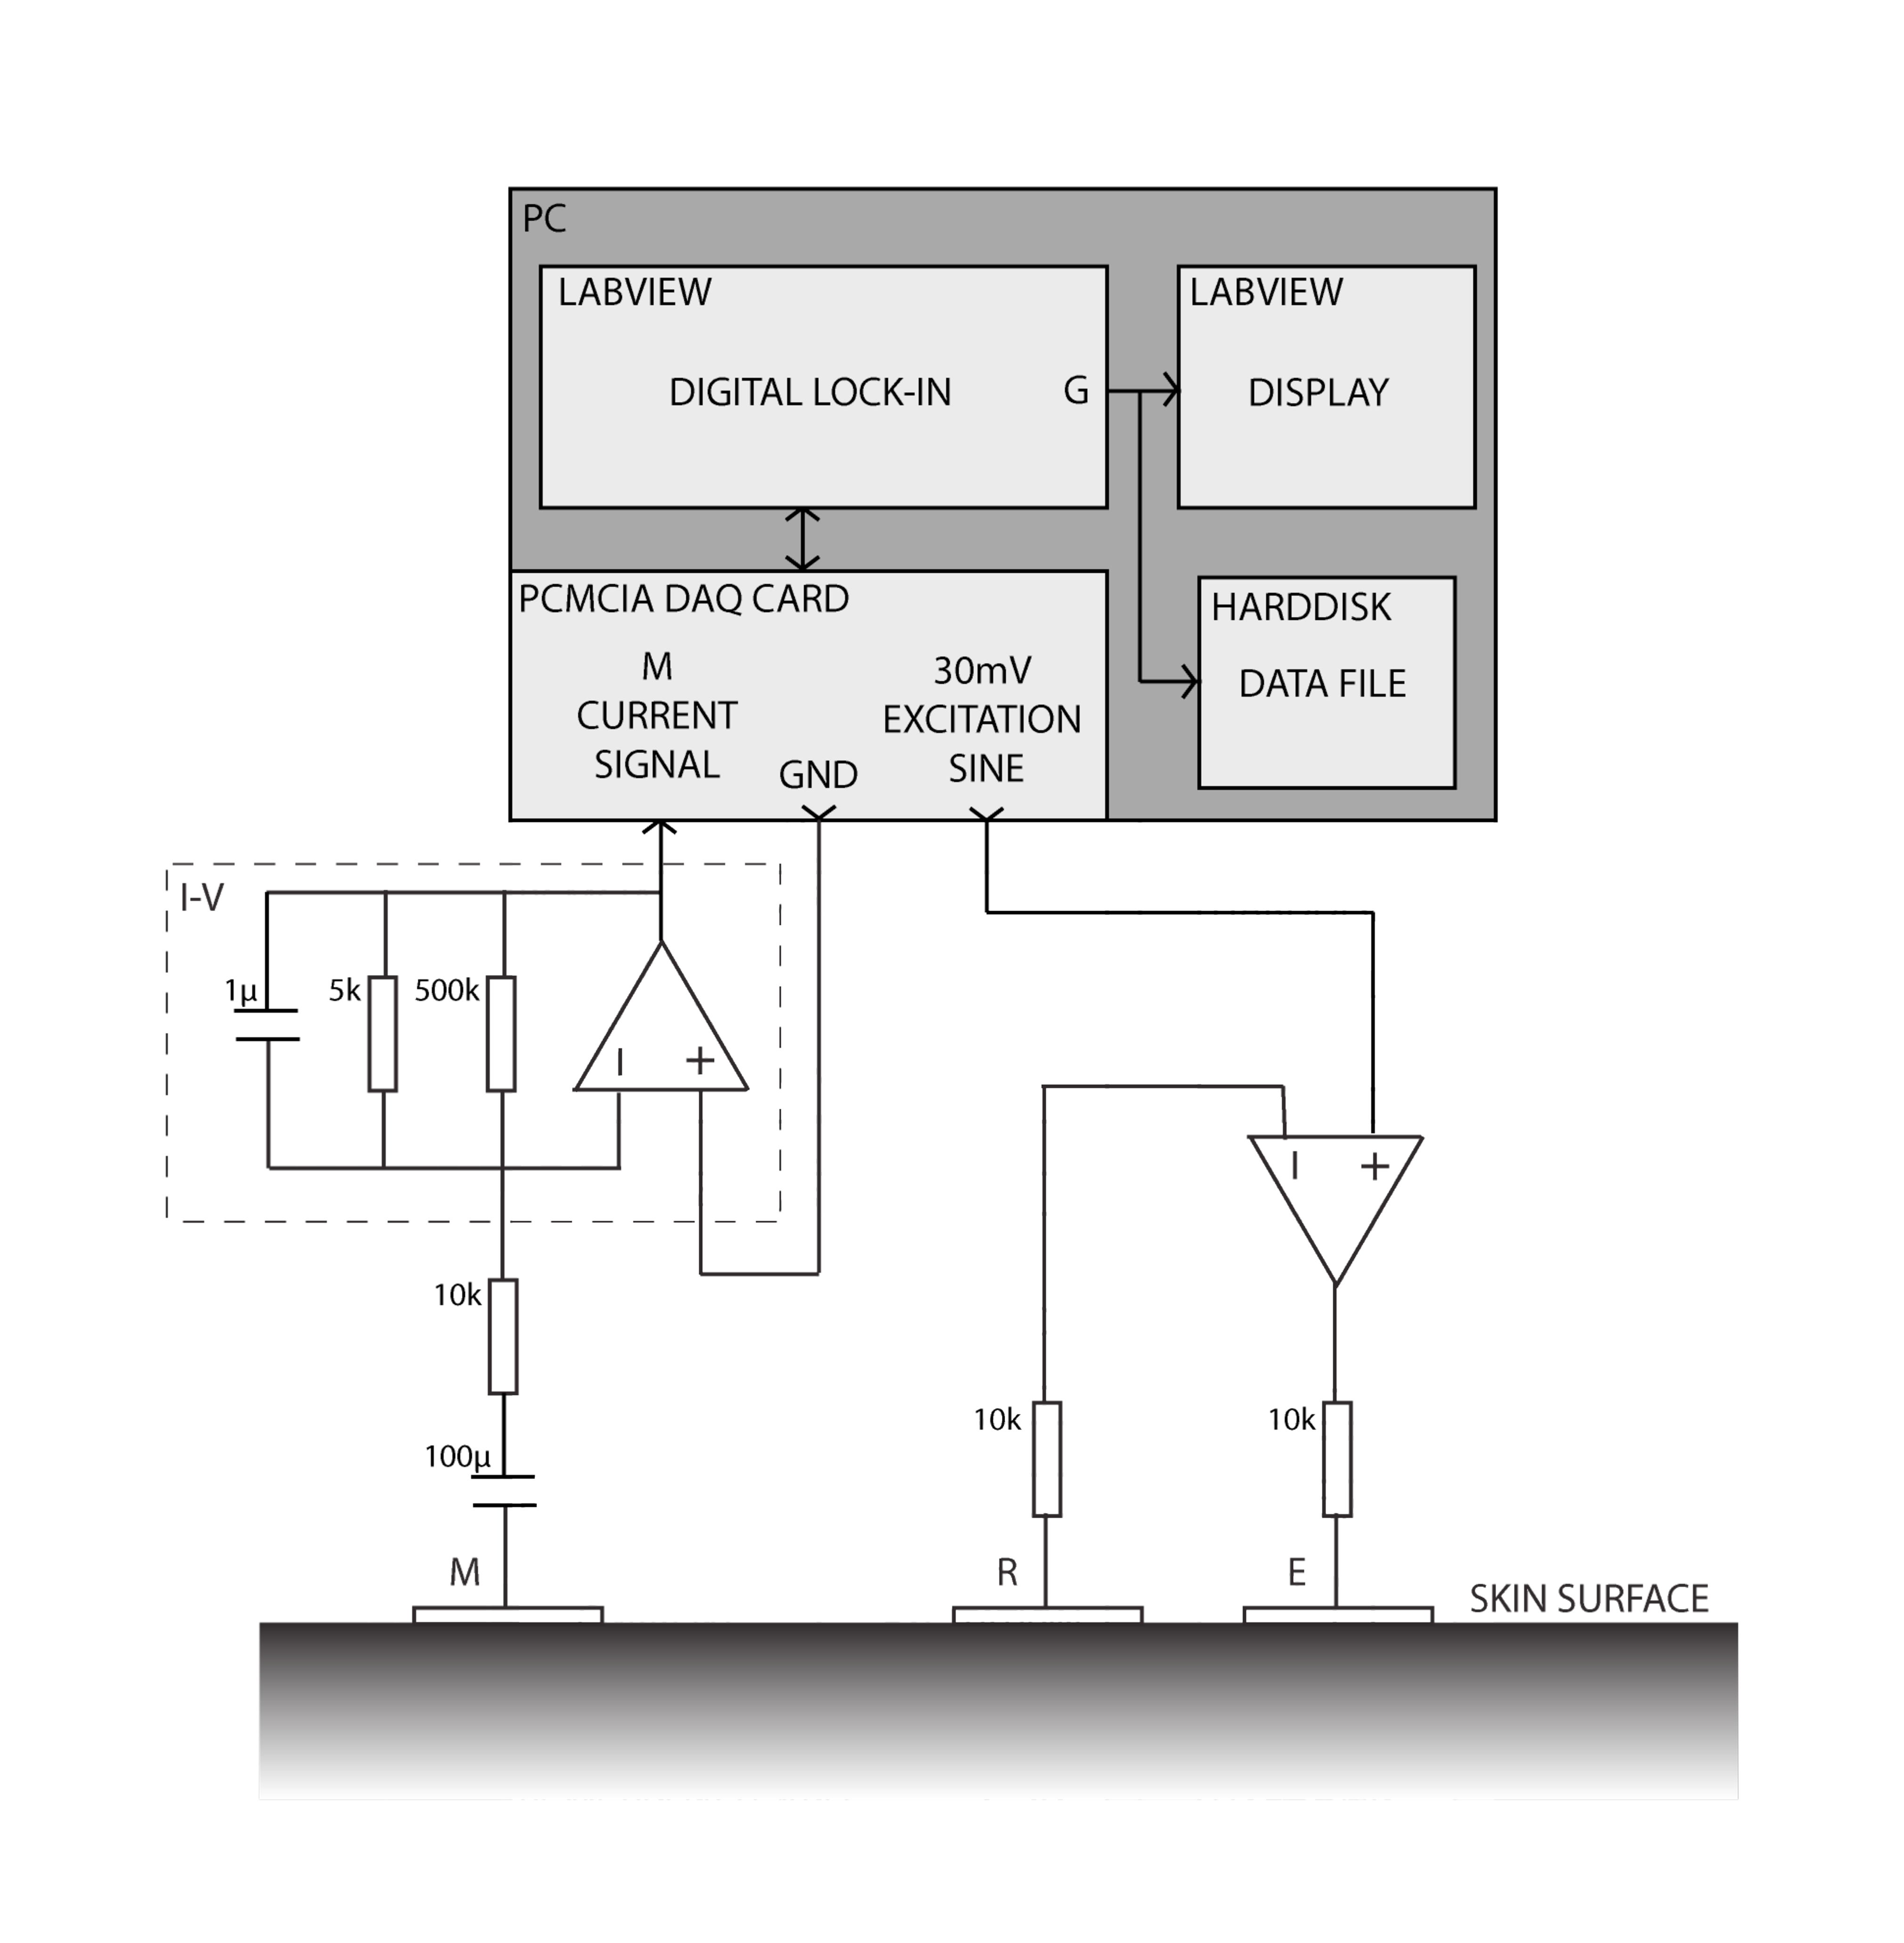
\includegraphics[scale=0.1]{Figurer/setup.pdf}
			\caption{ Measuring system for skin AC conductance. 
The system is composed of three main parts: 1.Skin surface electrodes creating the interface between electronic and ionic 
conductance. 2. Front-end electronics consisting of one dual op-amp IC, 5 resistors and two capacitors built into a small box 
(60x35x40mm). 3. A PC with a DAQ-card and software for signal processing, display and data storage. A 30mV sine voltage 
generated by the PC is applied to the skin through the E and R electrodes. Remote sensing at the current-less R electrode 
causes the right op-amp to drive a current through E which keeps the potential under R equal to the excitation sine, thus 
eliminating the stratum corneum impedance(SC) below E. Because the impedance of the wet tissue is negligible compared 
to that of the SC, the only current opposing element that is left is the impedance of the SC below the M electrode. Thus, the 
measurement is monopolar and confined to the SC of the effective electrode area below M, and the major contributor to 
changes in this impedance is the filling and reabsorption of sweat in the sweat ducts. The I-V dashed box on the left 
constitute a current to voltage converter with a Fc=200Hz RC lowpass filter. The 100� capacitor blocks DC potentials 
generated by the skin and electrodes. The digitized current signal is demodulated by the phase-corrected excitation sine in 
software, giving the AC conductance output to the display and the data file. For the electrodermal activity (EDA) 
measurements in this study, the M electrode was placed on the hypothenar area of 
the palm, while the R and E electrodes were placed on the underarm, but the placement of these two are not critical. }
		\end{figure}
	\end{center}

\subsection{Our stress measurements}
\newpage
\section{Stocastic processes and synthetic time series}
Let us now make a giant leap from the real world to world of theory. In order to be able to parameterize our measurements 
as outlined, we have to have an understanding of synthetic "measurements", realized by stochastic processes. The most 
fundamental class of such processes are the so-called stationary processes. We will review some basics about 
stationary processes and their spectral density function (SDF). But as mentioned in the introduction, these processes
do not suite our task well as a model for SA. Therefore we have to take a look at how we can develop non-stationary 
processes from a stationary processes. Finally we will briefly look at some popular synthetic time series and discuss
how to make a parameterization of them. 
	\subsection{Stationary stochastic processes}
	A process is said to be stationary if its statistical features do not change over time. Different segments of such 
	processes are more or less identical. To be more precise, we can define the real valued, discrete parameter 
	stochastic process $\{X_{t} : t=...,-1,0,1,...\}$ as a sequence of random variables. In order for $\{X_{t}\}$ to be
	stationary, it must satisfy the following properties
	$$
	E\{X_{t}\}=\mu_{X}\forall{t}
	$$
	$$
	cov\{X_{t},X_{t+\tau}\}=s_{X,\tau}\forall{t,\tau}
	$$
	The first property tells us that the expected value of the process equals a finite constant $\mu_{X}$ at any point $t$.
	The second property tells us that the covariance between any two components of $\{X_{t}\}$ equals a finite constant,
	$s_{X,\tau}$, that only depends on the separation between the components, $\tau$. The sequence of these 
	constants $\{s_{X,\tau} : \tau=...,-1,0,1,...\}$ is called the auto covariance sequence (ACVS). The second property 
	has two important implications of the elemnts in the ACVS
	$$
	s_{X,0}=cov\{X_{t},X_{t}\}=E\{\left({X_{t}-\mu_{X}}\right)^{2}\}=var\{X_{t}\}
	$$
	and
	$$
	s_{X,-\tau}=s_{X,\tau}
	$$
	The ACVS is very useful to know because we can define stochastic processes entirely by its ACVS. But for our 
	purpose it is more convenient to consider the Fourier transform of the ACVS. If the ACVS is square summable,
	we have
	\begin{equation}
	\label{sdf}
		S_{X}\left({f}\right)=\sum_{\infty}^{\infty}{s_{X,\tau}e^{-i2\pi{f}\tau}}\quad,-\frac{1}{2}\leq{f}\leq\frac{1}{2}
	\end{equation}
	This is called the spectral density function (SDF) of $\{X_{t}\}$. From our knowledge of the ACVS, we can state
	two important facts about the SDF:
	\begin{equation}
	\label{sdfprop1}
		S_{X}\left({-f}\right)=S_{X}\left({f}\right)
	\end{equation}
		\begin{equation}
	\label{sdfprop2}
		\int_{-1/2}^{1/2}{S_{X}\left({f}\right)df}=s_{X,0}=var\{X_{t}\}
	\end{equation}
	To summarize these two properties in a few words, we claim that the SDF is an even function that decomposes
	the process variance with respect to frequency. Another important property of the SDF is that the SDFs of two 
	stationary processes $\{X_{t}\}$ and $\{Y_{t}\}$, $\{Y_{t}\}$ created by linearly filtering $\{X_{t}\}$, are related by the 
	following formula
	\begin{equation}
	\label{sdfprop3}
		S_{Y}\left({f}\right)=\left|{T\left({f}\right)}\right|^{2}S_{X}\left({f}\right)
	\end{equation}
	where $T\left({f}\right)$ is the filter's transfer function. Because the integral of the SDF is the process variance, we 
	must also have
	\begin{equation}
	\label{sdfprop4}
		var\{Y_{t}\}=\int_{-1/2}^{1/2}{S_{Y}\left({f}\right)df}=
		\int_{-1/2}^{1/2}{\left|{T\left({f}\right)}\right|^{2}S_{X}\left({f}\right)df}
	\end{equation}
	The SDF and its properties are crucial for the theory reviewed in the remaining of this chapter and chapter 5.
	\subsection{Non-stationary processes}
	In the previous section we looked at stationary processes and an important function, the SDF, characterizing them.
	As we know, the nature of the SA signals is non-stationary, so it is of interest to define a class of non-stationary 
	processes which can be used as a model for the SA signals. We will now look at a way to ensure a well-defined SDF 
	for a class of non-stationary processes, the so-called $1/f$-type processes.
	\\
	\\
	Let us consider the stochastic process $\{X_{t}\}$ whose $dth$ order backward difference
	\begin{equation}
	\label{bwd}
		Y_{t}\equiv\left({1-B}\right)^{d}X_{t}=\sum_{k=0}^{d}{d\choose{k}}\left({-1}\right)^{k}X_{t-k}\quad,d\in\mathbb{N}_{0}
	\end{equation}
	is a stationary process with SDF $S_{Y}$ and mean $\mu_{Y}$. The backward shift operator $B$ is defined as
	\begin{equation}
	\label{bop}
		B^{k}X_{t}=X_{t-k}
	\end{equation}
	If $\{X_{t}\}$ is stationary, the SDFs are related through equation ($\ref{sdfprop3}$). If $\{X_{t}\}$ is not stationary, 
	however, we can define
	\begin{equation}
	\label{nonstatSDFprop}
		S_{Y}\left({f}\right)=\left|{D\left({f}\right)^{d}}\right|^{2}S_{X}\left({f}\right)
	\end{equation}
	where $D\left({f}\right)$ is the transfer function of the backward difference filter. This definition ensures a well defined 
	SDF for the non-stationary process because ($\ref{bwd}$) tells us that the stationary process, having a well-defined 
	SDF, can be constructed by backward shifts of the non-stationary process. For the special case $d=1$, we have
	$$
	\left|{D\left({f}\right)}\right|^{2}=4\sin^{2}\left({\pi{f}}\right)
	$$
	\subsection{Long memory processes}
	We will now define the concept of having memory built into a process and redefine the hypothesis given in the introduction
	according to this. A process is said to hold long range dependency, or memory, if it satisfies
	\begin{equation}
	\label{lmp}
		\mathop{\lim}\limits_{f\to{0}}\frac{S_{X}\left({f}\right)}{C\left|{f}\right|^{\alpha}}=1
	\end{equation}
	where $C>0$ and $\alpha<0$ is constant. We can assign a parameter like $\alpha$ to any long memory process 
	(LMP). The SDF for a LMP must be a function of this paramater, so this parameter, which we will call the LMP parameter, is 
	related to the appearance of the LMP itself. In the view of our SA measurements, we can imagine a model where a 
	provocation forces the signal to be a LMP. Then the signal will "remember" this provocation and this will affect the 
	appearance of the measured signal until it is completely relaxed. We can then assume that the LMP parameter is constant 
	for a relatively short period of time\footnote{Relatively short compared to the time it takes to completely relax the system.}. 
	Our hypothesis is then
	\\
	\\
	\emph{The LMP parameter inherent in EDR-measurements of SA at the hypothenar is correlated to experienced stress }
	\subsection{Synthetic time series}
	As we have redefined our hypothesis, we are now on the hunt for a model of a non-stationary LMP. Luckily, we are 
	able to construct non-stationary stochastic processes with well-defined SDFs through stationary stochastic processes, so a 
	suitable model is in sight. In this section we will look at some widely used stochastic processes and choose a suitable 
	processes as a model for our SA-measurements. Let us start out by examine some popular stationary LMPs studied in the 
	litterature. 
	\newpage
	\subsubsection{Stationary models}
	\emph{Pure power law processes}
	\\
	The discrete-parameter, stationary stochastic process $\{X_{t}\}$ is said to be a pure power law (PPL) process if its SDF
	has the form
	\begin{equation}
	\label{ppl}
		S_{X}\left({f}\right)=C\left|{f}\right|^{\alpha}\quad,-\frac{1}{2}\leq{f}\leq\frac{1}{2}
	\end{equation}
	where $C>0$ and $-1<\alpha<0$. This is perhaps the simplest model of a LMP because of its close relationship to the 
	definition of LMP given in equation ($\ref{lmp}$). As a consequence of this definition, a PPL is not a LMP for $\alpha\geq{0}$.
	The SDF of the PPL process is plotted in figure ???.
	\\
	\\
	\emph{Fractional Gaussian noise}
	\\
	The historically oldest model of a LMP is the fractional Gaussian noise (FGN). Although aging, it is a widely used 
	model for physiological signals (Eke et al.(2002)). It is typically defined through its ACVS. The discrete, stationary 
	process $\{X_{t}\}$ is a FGN if its ACVS is
	\begin{equation}
	\label{fgnacvs}
		s_{X,\tau}=\frac{\sigma_{X}^{2}}{2}\left({\left|{\tau+1}\right|^{2H}-2\left|{\tau}\right|^{2H}+\left|{\tau-1}\right|^{2H}}\right)
		\quad,\tau=...,-1,0,1,...
	\end{equation}
	where $\sigma_{X}^{2}=var\{X_{t}\}$, and $H$ is the Hurst exponent satisfying $0<H<1$. The SDF of FGN is a bit more 
	complicated and non-intuitive. It is given as
	\begin{equation}
	\label{fgn}
		S_{X}\left({f}\right)=\sigma_{X}^{2}C_{H}4\sin\left({\pi{f}}\right)\sum_{j=-\infty}^{\infty}{\frac{1}{\left|{f+j}\right|^{2H+1}}}
		\quad,-\frac{1}{2}\leq{f}\leq\frac{1}{2}
	\end{equation}
	where $C_{H}=\Gamma\left({2H+1}\right)\sin\left({\pi{f}}\right)/\left({2\pi}\right)^{2H+1}$. For small $f$ we have
	 $S_{X}\left({f}\right)\propto\left|{f}\right|^{1-2H}$. From equation ($\ref{lmp}$) we must require $1-2H<0$ in order for the 
	 FGN to be a LMP. This implies that FGN is a LMP when $0.5<H<1$. In this domain, low frequency components are 
	 becoming increasingly dominant as $H$ increases. For $0<H<0.5$ it is the other way around. In this domain high frequency 
	 components become increasingly dominant as $H$ decreases. In the special case $H=0.5$, equation ($\ref{fgnacvs}$) 
	 reduces to
	 \begin{equation}
	 \label{wn}
	 	s_{X,\tau}=\begin{cases}\sigma_{X}^{2}, & \tau=0\\0, & \mbox{ otherwise}\end{cases}
	 \end{equation}
	 This often referred to as a white noise process, $\{\epsilon_{t}\}$.
	\\
	\\
	\emph{Fractionally differenced processes}
	\\
	This white noise process is the mother of another popular time series model, the fractionally differenced (FD) process. We 
	can define a discrete FD process $\{X_{t}\}$ as 
	\begin{equation}
		\label{fddef}
		\left({1-B}\right)^{\delta}X_{t}=\sum_{k=0}^{\infty}{\delta\choose{k}}\left({-1}\right)^{k}X_{t-k}=\epsilon_{t}
	\end{equation}
	where $B$ is the backward shift operator of equation ($\ref{bop}$). Because a FD with LMP parameter $\delta=0$ is 
	equivalent to an FGN with LMP $H=0.5$, we must require $0<\delta<0.5$ to ensure that  the FD process is stationary 
	and a LMP. The SDF of such process can be obtained by applying equation ($\ref{nonstatSDFprop}$) to the SDF of the
	white noise process. If we denote $\sigma_{\epsilon}^{2}$ as the variance of the white noise process, the SDF of a FD 
	process has the form
	\begin{equation}
	\label{fd}
		S_{X}\left({f}\right)=\frac{\sigma_{\epsilon}^{2}}{\left[{4\sin^{2}\left({\pi{f}}\right)}\right]^{\delta}}
		\quad,-\frac{1}{2}\leq{f}\leq\frac{1}{2}
	\end{equation}
	\\
	\\
	We have now looked at three popular models for stationary LMPs. They are similar in the sense that they depend on two 
	parameters only, the variance of the process and the LMP parameter. For us this exponent is of particular interest. The 
	following figure will give us an idea how to extract the LMP parameter from the SDF.
	\newpage
	\begin{center}
		\begin{figure}[!h]
			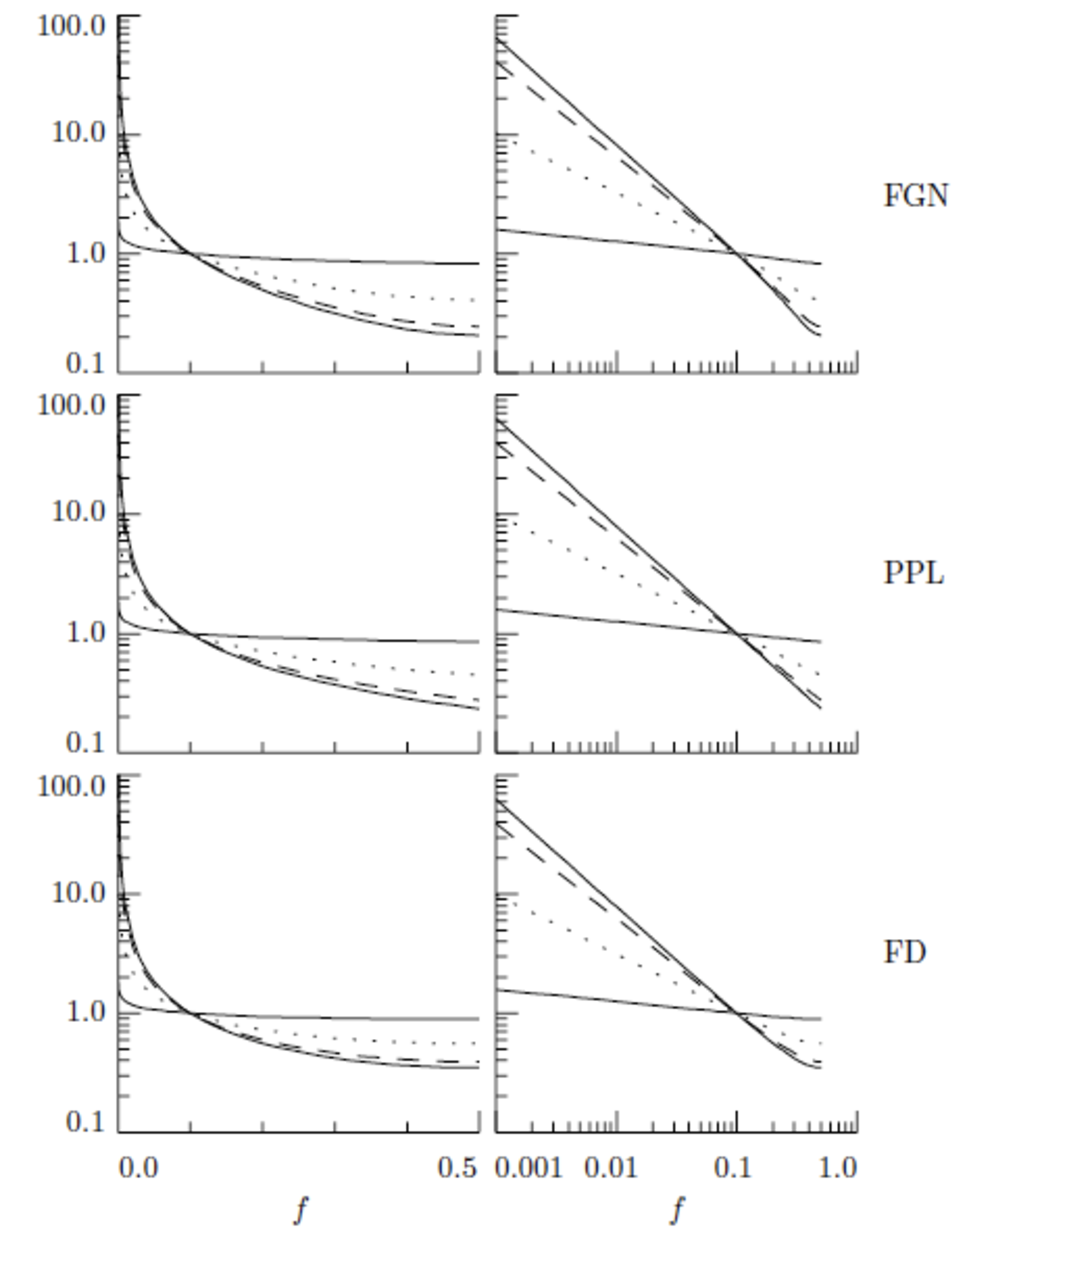
\includegraphics[scale=0.6]{Figurer/SDF.pdf}
			\caption{SDFs for FGN, PPL and FD processes plotted linearly and as log/log. They are normalized such that 
			$S_{X}\left({0.1}\right)=1$. The SDFs are plotted with LMP parameter values equivalent to $\alpha=-0.1$ (thick 
			solid line), $\alpha=-0.5$ (dotted line), $\alpha=-0.8$ and $\alpha=-0.9$. The relationship between the LMP 
			parameters are given in Figure ???.}
		\end{figure}
	\end{center}
	As we can see, the SDF of a PPL process is completely linear in a log/log plot, and we can easily extract the LMP parameter 
	by the slope of its SDF. The FGN and FD processes have an approximately linear SDF below about $f=0.2$ and $f=0.1$ 
	respectively. By skipping the highest frequencies, we can extract the LMP parameters by the slope of this segment of the 
	SDF.   
	\subsubsection{Non-stationary models}
	We can extend the theory of synthetic time series to include non-stationary LMPs as well. Let us generalize the theory 
	reviewed above.
	\\
	\\
	\emph{Pure power law processes}
	\\
	From the definition of a PPL process given in equation ($\ref{ppl}$), there is nothing restricting us from allowing other values 
	of $\alpha$ than the ones ensuring the PPL process to be stationary. $\alpha$ is in fact defined over the entire real axis, but 
	because of the definition of a LMP, we must have $\alpha<0$ in order to have a PPL process with long range memory. Now 
	given the range of $\alpha$ defining a stationary process, we can argue that $\alpha\leq{-1}$ yields a non-stationary PPL 
	process. The non-stationary PPL process will still have a well-defined SDF which is completely linear in a log/log plot.
	\\
	\\
	\emph{Fractionally differenced processes}
	\\
	In a similar manner, we can argue that there is nothing in the definition of a FD process given in equation ($\ref{fd}$) 
	restricting the LMP parameter $\delta$ to be in the range $0<\delta<0.5$, as we needed to construct a stationary FD process.
	$\delta$ is, like $\alpha$, defined over the entire real axis. So in order to have a non-stationary FD process with long range 
	memory, it is sufficient to choose $\delta\geq{0.5}$.
	\\
	\\
	\emph{Fractional Brownian motion}
	\\
	In contrast to the LMP parameters of PPL and FD processes, being defined over the entire real axis, the LMP parameter of 
	an FGN process is restricted to a finite interval. So we cannot generalize the FGN to be a non-stationary process. It is 
	stationary by definition! Luckily, we are able to construct non-stationary processes from stationary processes by backward 
	difference ($\ref{bwd}$). A very popular model of a non-stationary process is constructed by taking the first order backward 
	difference of the FGN process. This is called fractional brownian motion (FBM). The SDF of a discrete, real valued FBM 
	process $\{X_{t}\}$ is given as
	\begin{equation}
	\label{fbm}
		S_{X}\left({f}\right)=\sigma_{X}^{2}C_{H}\sum_{j=-\infty}^{\infty}{\frac{1}{\left|{f+j}\right|^{2H+1}}}
		\quad,-\frac{1}{2}\leq{f}\leq\frac{1}{2}
	\end{equation}
	where $C_{H}=\Gamma\left({2H+1}\right)\sin\left({\pi{f}}\right)/\left({2\pi}\right)^{2H+1}$ as before. The FBM is a model that
	has a lot of different applications. It has a natural link to fractal theory, and the fractal dimension $D$ is related to the Hurst
	exponent of a FBM process as
	\begin{equation}
	\label{fracdim}
		D=2-H
	\end{equation}
	It has been widely used as a model for physiological signals too. Eke et al. (2002) suggests that any non-stationary 
	physiological signal should be modeled as FBM. Hence the FBM model, with its LMP parameter $H$, is a natural choice of 
	model for our SA measurements. To test our hypothesis, we need a mathematical tool to extract the Hurst exponent from our 
	measurements. The theory needed to do so will be described in the following two chapters. 
	\\
	\\
	\begin{center}
		\begin{figure}[!h]
			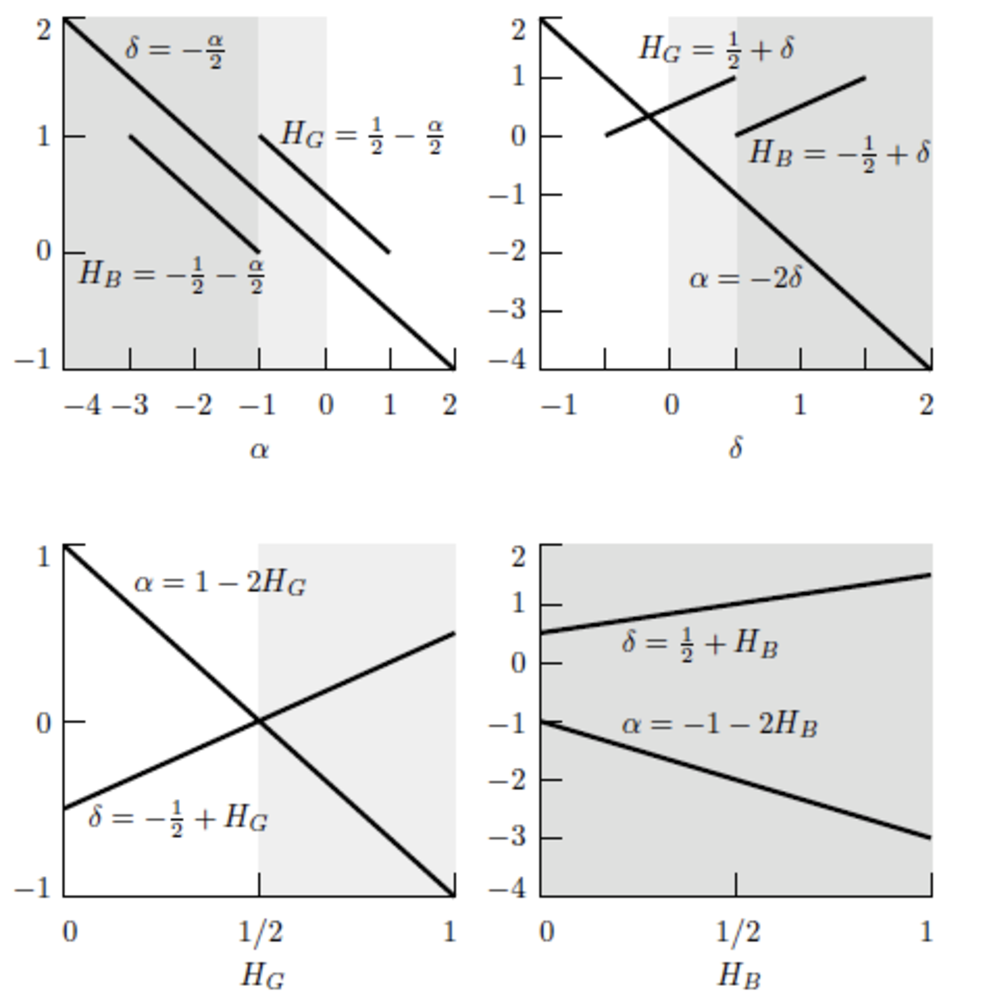
\includegraphics[scale=0.7]{Figurer/LMP.pdf}
			\caption{Relationships between LMP parameters of the models reviewed here. In order to separate between
			the Hurst parameters of FGN and FBM, we denote the Hurst exponent of a FGN process as $H_{G}$ and the 
			Hurst exponent of a FBM process as $H_{B}$. The white areas in the figure represent parameter values
			corresponding to processes without long memory, the lightly shaded areas correspond to processes with
			"short" memory and the the heavily shaded areas correspond to a LMP.}
		\end{figure}
	\end{center}
\newpage
\section{The wavelet transform}
We constructed a model where a provocation sets a value to the LMP parameter, yielding a characteristic shape of the measured
signal for a short period of time. We need to decompose the signal so that we finally can fit a regression line, skipping the highest frequencies.
The purpose of this thesis is to assign a parameter to the measured SA-signals. In order to do this, we will need a
mathematical tool well suited to analyze non-stationary time series as realized by the SA measurements. I will start out by 
defining the Fourier transform and %And WFT who, but limited precision of both time/frequency at the same time
the wavelet transform in the contineous...
\\
\\
As we have seen, the time series are discrete sampled in time. It is often, however, more convenient to . 
to look for discrete transform.  FT decompose over scale yield a SDF...?
then the main objective of this chapter is to find a fast 
implementation of the discrete transform. 
Will stick to 1D throughout\\
MRA = scale instead of frequency\\
I will assume real wavelets (although a generalization is no problem (thus innerproduct -> integral form no *)\\
	\subsection{The Fourier transform}
		To extract the frequency information of a signal $f$ in the time domain, a standard technique is to use the
		Fourier transform (FT):
		\begin{equation}
			\label{FT}
			\hat{f}(\omega)=\int_{-\infty}^{\infty}{f(t)e^{-i\omega t}dt}		
		\end{equation}
		Where $\hat{f}\left({\omega}\right)$ is a representation of $f$ in the frequency domain. We can transform $f$ 
		back to the time domain by the inversion
		\begin{equation}
			\label{iFT}
			f\left({t}\right)=\frac{1}{2\pi}\int_{-\infty}^{\infty}{\hat{f}\left({\omega}\right){e^{i\omega{t}}}d\omega}
		\end{equation}
		The FT measures "how much" oscillations are at the frequency $\omega$ there is in $f$, but does not give
		much information about at which times the frequencies occures. Time-localization can be achieved by first
		windowing the signal $f$ by a function $g$, so as to cut off only a well-localized slice of $f$, and then take its 
		FT:
		\begin{equation}
			\label{WFT}
			\hat{f}(\omega,t)=\int_{-\infty}^{\infty}{f(s)g(s-t)e^{-i\omega s}ds}
		\end{equation}
		This is known as the windowed Fourier transform (WFT). The transform is highly redundant, representing a one
		dimensional signal in the time-frequency plane ($\omega, t$). It can be interpreted as the "content" of $f$ near
		time $t$ and near frequency $\omega$. Although the WFT yields a time-frequency decomposition of the signal, 
		it's not necessarily a good tool for an analysis of an arbitrary signal. The WFT decomposes signals over 
		waveforms that have the same time and frequency resolution.	If the signal of interest includes structures having 
		different time-frequency resolutions we will need another tool that adress this issue. This leads to the wavelet 
		transform.
	\subsection{The continuous wavelet transform}
		To define a transformation that can handle a varying time-frequency resolution, we will need an analyzing
		function that is localized in time and frequency as opposed to the complex exponentials (or equivalently sine/
		cosine) used in FT and WFT. We can obtain this using wavelets. 
		%We can construct such basis using wavelets. %blabla see what wavelets
		%are and how do a CWT...?
		\subsubsection{Wavelets}
			Let us define a function $\psi$(t) of the real variable $t$ with properties
			\begin{equation}
				\label{waveprop1}
				\int_{-\infty}^{\infty}\psi(t)dt=0
			\end{equation}
			\begin{equation}
				\label{waveprop2}
				\int_{-\infty}^{\infty}\psi^2(t)dt=1
			\end{equation}	
			If ($\ref{waveprop1}$) and ($\ref{waveprop2}$) is satisfied, $\psi$(t) resembles a wave localized in time, a 
			wavelet. A family of wavelets can then be constructed by translating and dilating our mother wavelet
			\begin{equation}
				\label{waveletfamily}
				\psi_{a,b}(t)=\left| a\right|^{-\frac{1}{2}}\psi\left(\frac{t-b}{a}\right)\quad ,\quad a,b\in\mathbb{R},a\neq 0
			\end{equation} 
			where $a$ is the dilation parameter and $b$ is the translation parameter. Let us take a closer look at how
			typical wavelets may look like. 
			\clearpage
			\begin{center}
				\begin{figure}[!h]
					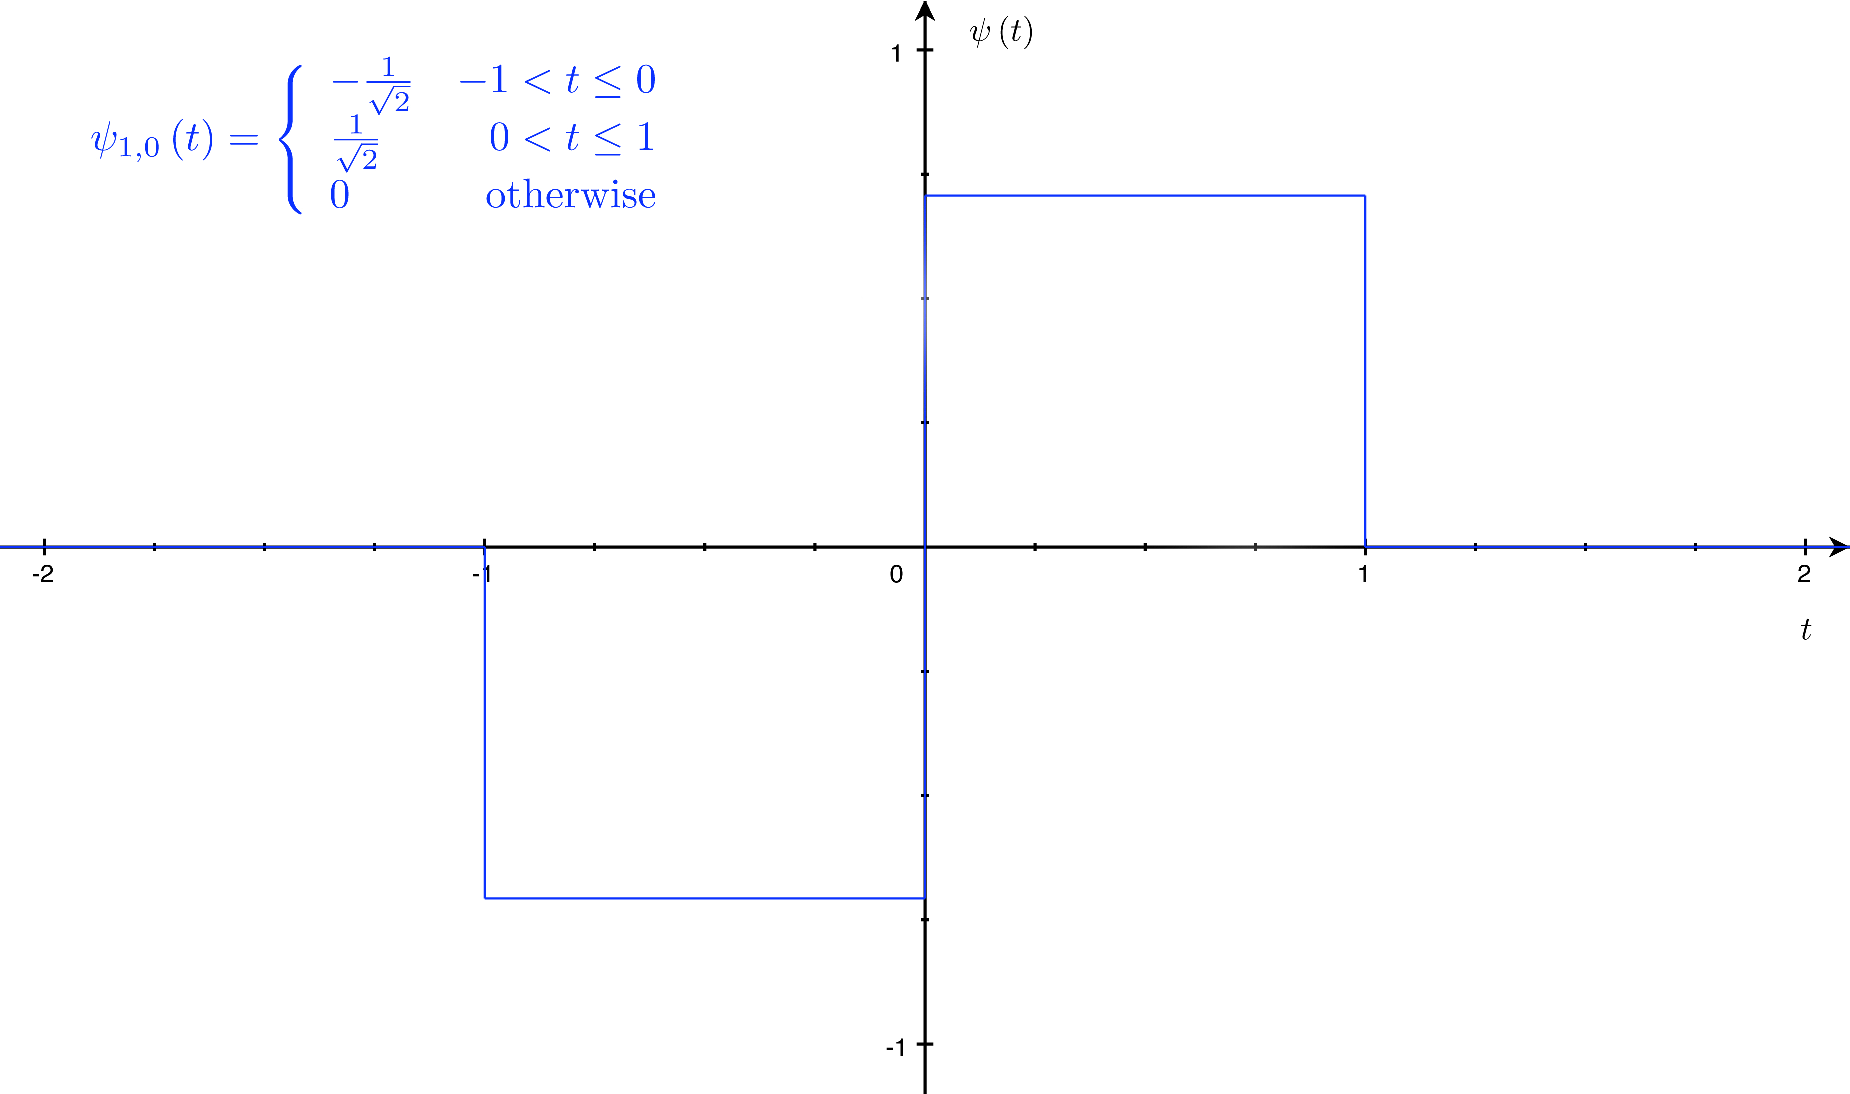
\includegraphics[scale=0.4]{Figurer/Haar.pdf}
					\caption{The Haar wavelet. This was the first wavelet to be discovered and it had nothing to do 
					with wavelet theory in the first place. Alfred Haar used this function to create a orthonormal 
					system in $L^{2}\left(\mathbb{R}\right)$. It was "rediscovered" when the wavelet theory was 
					developed in the 1980s. As we will see later, this is the simplest wavelet of a class of wavelets 
					discovered by Daubechies.}
				\end{figure}
			\clearpage
				\begin{figure}[h]
					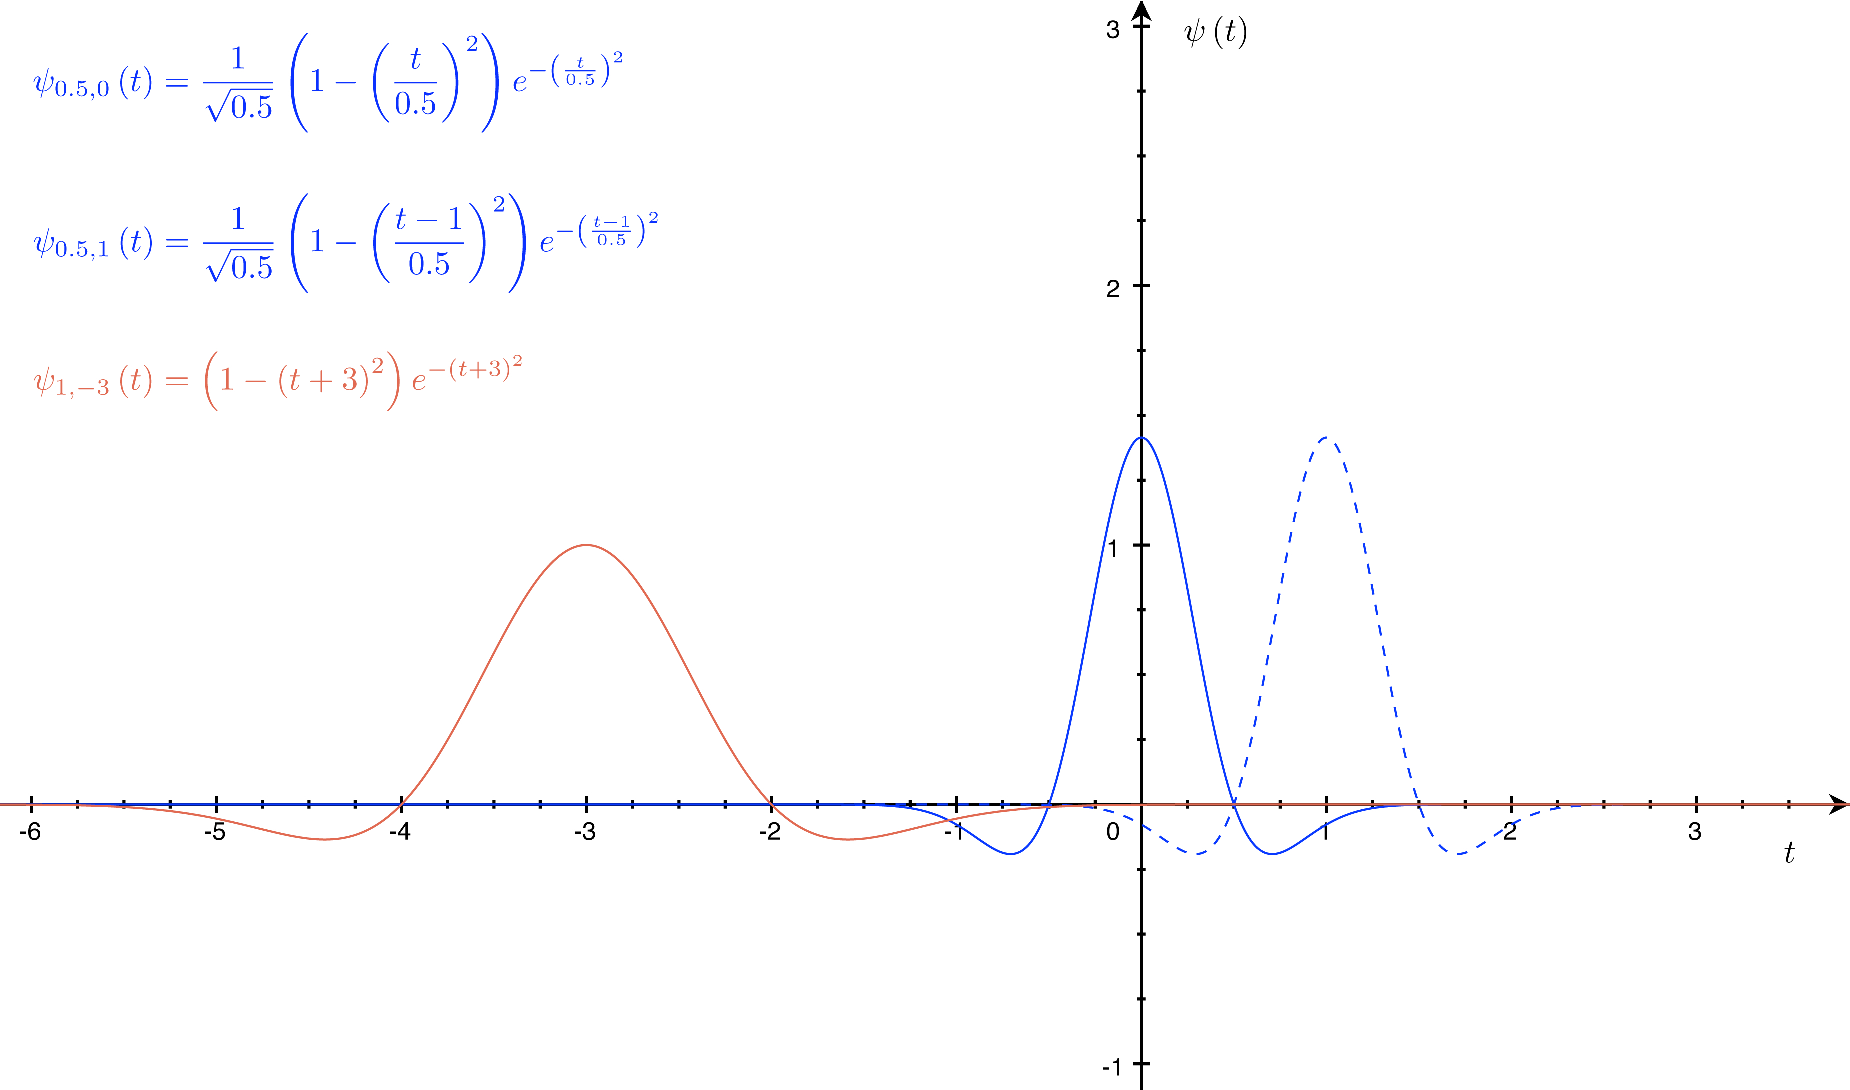
\includegraphics[scale=0.4]{Figurer/MexicanHat.pdf}
					\caption{Mexican Hat wavelets. The second derivative of a Gaussian. I have plotted...Nanana}
				\end{figure}
			\end{center}
		\subsubsection{CWT}
			Now that we have an idea of what a wavelet is, we can finally define the continuous wavelet transform 
			(CWT). The transform analogous to ($\ref{WFT}$) using wavelets is
			\begin{equation}
				\label{CWT}
				W(a,b)=\int_{-\infty}^{\infty}f(t)\psi_{a,b}(t) dt
			\end{equation}
			Which indeed is a highly redundant transform like the WFT. Basically the only thing we have done is to 
			substitute the analyzing functions $g_{\omega,t}(s)=g(s-t)e^{-i\omega s}$ with $\psi_{a,b}(t)$. By doing so 
			we achieve what we were looking for. With the functions $g_{\omega,t}$ we were stuck with the envelope 
			function $g$, which regardless of $\omega$ had the same width. $\psi_{a,b}$, on the other hand, are able 
			to adapt its width to the frequency in the signal. High frequency $\psi_{a,b}(t)$ are very narrow, while low 
			frequency $\psi_{a,b}(t)$ are much broader.Thus the wavelet transform is better able to "zoom in" on high 
			frequency phenomena than theWFT.
			\\
			\\
			Equation ($\ref{CWT}$) is the analysis of the signal $f$(t), and our motivation for constructing the family of
			wavelets $\psi_{a,b}$. A synthesis of the signal is possible and given by the formula
			\begin{equation}
				\label{iCWT}
				f(t)=\frac{1}{C_{\psi}}\int_{-\infty}^{\infty}\int_{-\infty}^{\infty}W(a,b)\psi_{a,b}(t)\frac{da db}{a^2}
			\end{equation}
			Here we require a further restriction of our wavelets in order to allow reconstruction of $f$, the so-called 
			admissibility condition. A wavelet $\psi(t)$ is said to be admissible if its FT is such that
			\begin{equation}
				\label{admissibility}
				C_{\psi}\equiv\int_{0}^{\infty}\frac{\left|\hat{\psi}(t)\right|^2}{\left|t\right|}<\infty
			\end{equation}
		%Oppsummere, nevne det mentale bildet med en lokalisert b�lge som ser etter informasjon i signalet simultant 
		%p� alle skalaer og transleres i signalet. CWT gir da et bilde av f i (a,b) planet
	\subsection{Discretization of the wavelet transform}
		In order to obtain an efficient numerical implementation of the wavelet transform, we have to derive a discrete
		version of it. Let us consider a discretization of the CWT in the (a,b) plane introducing discrete wavelets.
		\subsubsection{Discrete wavelets}
			We can define a family of discrete wavelets by allowing the dilation parameter $a$
			and the translation parameter $b$ both to take discrete values only. If we choose $a=a_{0}^j$
			and $b=kb_{0}a_{0}^j$, where $b_{0}>0$ and $j,k\in\mathbb{Z}$, we ensure that the 
			discretized wavelets $\psi_{j,k}$ "cover" $t$ in the same way for all $j$. The family of discrete wavelets 
			is then
			\begin{equation}
			\label{dwb}
				\psi_{j,k}(t)=a_{0}^{-\frac{j}{2}}\psi(a_{0}^{-j}t-kb_{0}) %m,n looks nicer...
			\end{equation} 
			The analysis of a signal $f$ is given by
			\begin{equation}
				\label{discreteWT}
				W(j,k)=\int_{-\infty}^{\infty}f(t)\psi_{j,k}(t) dt
			\end{equation}
			This description yields yet again a redundant transform. However, the discrete wavelets defined in 
			($\ref{dwb}$) does not in general give rise to a synthesis equation like ($\ref{iCWT}$) even if the 
			admissibility condition ($\ref{admissibility}$) is satisfied in its discrete form. A solution to this problem can 
			be approached in two ways:
			\\
			\\$\bullet$\quad Construct wavelets $\psi_{j,k}$ who constitute a frame \footnote[1]{A frame of a vector
			space can be seen as a generalization of the idea of a basis to sets which may be linearly dependent}
			\\$\bullet$\quad Construct an orthonormal wavelet basis with compact support
			\\
			\\
			The first approach is carefully studied in (daub and mallat). If we follow this path, we will typically end up 
			choosing wavelets who are well localized in time and frequency, but defined over the entire real axis. To 
			implement such a transform, we will have to make a cut-off of the wavelets at some point. It would be more 
			convenient to implement a transform whose wavelets have compact support. This can be achieved by 
			constructing an orthonormal wavelet basis. Our first step towards a numerical implementation of the 
			wavelet transform is thus to create such basis. To get there, we will have to define the concept of a 
			multiresolution approximation.		
		\subsubsection{Multiresolution approximation}
			%F� med at delen av signalet i et subspace tilsvarer en range av frekvenser og at dette er relatert til a??
			Let us consider a function space decomposed into a ladder of subspaces where each
			subspace is a scaled version of the central space. If we look at our signal $f$ this way, it implies that
			there is a piece of $f$ in each subspace. An orthogonal projection of $f$ on subspace $V_{j}$ will give an 
			approximation $f_{j}$ of $f$ at resolution $a_{0}^{-j}$. If we let $\{W_{j}\}$ be another family of 
			subspaces containing the differences between $V_{j-1}$ and $V_{j}$ for all $j$, then $f$ can be 
			approximated at an arbitrary precision by $\{V_{j}\}$ and $\{W_{j}\}$. Let us give these ideas a more 
			mathematical framework. For simplicity, we choose $a_{0}=2$ and $b_{0}=1$, which means that 
			($\ref{dwb}$) takes the form
			\begin{equation}
				\label{odwb} 
				\psi_{j,k}(t)=2^{-\frac{j}{2}}\psi(2^{-j}t-k)
			\end{equation}
			A multiresolution approximation is then a sequence of closed subspaces $\{V_{j}\}$ satisfying the 
			following properties
			\begin{equation}
				\label{mra1}
				V_{j}\subset{V_{j-1}}\quad,\forall{j\in\mathbb{Z}}
			\end{equation}
			\begin{equation}
				\label{mra2}
				\overline{\bigcup_{j\in\mathbb{Z}}{V_{j}}}=L^2(\mathbb{R})
			\end{equation}
			\begin{equation}
				\label{mra3}
				\bigcap_{j\in\mathbb{Z}}{V_{j}}=\{0\}
			\end{equation}
			\begin{equation}
				\label{mra4}
				f\in{V_{j}}\Longleftrightarrow f(2^j\cdot)\in{V_{0}}\quad,\forall j\in\mathbb{Z}			
			\end{equation}
			\begin{equation}
				\label{mra5}
				f\in{V_{0}}\Rightarrow f(\cdot -k)\in V_{0}\quad ,\forall{k\in\mathbb{Z}}
			\end{equation}
			\begin{equation}
				\label{mra6}
				\exists\phi\in{V_{0}}:\{\phi_{0,k} ;k\in\mathbb{Z}\} \mbox{ is an orthonormal basis}
			\end{equation}
			To summarize these equations in a few words, equations ($\ref{mra1}$), ($\ref{mra2}$), ($\ref{mra3}$)
			ensures completeness of $\{V_{j}\}$ in $L^2(\mathbb{R})$, equation ($\ref{mra4}$) require $V_{j}$ to be
			scale invariant and equation ($\ref{mra5}$) require $V_{j}$ to be shift-invariant. Equation ($\ref{mra6}$)
			combined with ($\ref{mra4}$) tells us that there for all $j,k\in\mathbb{Z}$ exist an orthonormal basis 
			$\{\phi_{j,k}\}$ where
			\begin{equation}
				\label{scalingfunction}
				 \phi_{j,k}(t)=2^{-\frac{j}{2}}\phi(2^{-j}t-k)
			\end{equation}
			We will call $V_{j}$ the scaling space, hence $\phi_{j,k}$ is called the scaling function of the 
			multiresolution approximation. Let $W_{j}$ be the wavelet space with an orthonormal wavelet basis 
			$\{\psi_{j,k};j,k\in\mathbb{Z}\}$. For all $j\in\mathbb{Z}$ we define 
			\begin{equation}
				\label{ws}
				V_{j-1}=V_{j}\bigoplus{W_{j}}
			\end{equation}
			with the constraint that $W_{j}\perp{W_{j'}}$ if $j\neq{j'}$. We see that $W_{j}$ contain the difference 
			between the approximations with resolution $2^{j-1}$ and $2^{j}$. We will call this the detail at level $j$. 
			Using equation ($\ref{mra2}$) we can "telescope" the union to write
			\begin{equation}
				\label{waveletdecomp}
				L^2(\mathbb{R})=\bigoplus_{j\in\mathbb{Z}}{W_{j}}
			\end{equation}
			In other words, the wavelet subspaces yields a wavelet decomposition of $L^2(\mathbb{R})$! Equations
			($\ref{mra2}$), ($\ref{mra3}$) and ($\ref{waveletdecomp}$) then implies that $\{\psi_{j,k};j,k\in\mathbb{Z}\}$ 
			is a basis for $L^2(\mathbb{R})$. As a consequence of  ($\ref{ws}$), $W_{j}$ inherit the scaling property ($
			\ref{mra4}$) from $V_{j}$. Our search for an orthonormal wavelet basis can then be reduced to find 
			$\psi\in{W_{0}}$ such that $\psi{(\cdot -k)}$ constitute an orthonormal basis for $W_{0}$. 
			%Got to get 5.1.7 in here some place... (Den er igrunn innebakt i ws dersom man ser det i sammenheng
			%med det jeg sier i introen...
			%Mention a bit clearer that j-1 is a finer resolution than j.
				%Approximate f at scales... View wavelet-transform as averages and differences
		\subsubsection{The scaling function}
		Husk dette med averages/differences og hvilket nivaa naa!!!
			%!!!!!!!!!!!! Averages at level j (similarly waveletfunction differences at level j-1 (details))
			%Stick to omega as the frequency??? I use xi here!!!
			%Must show that g is orthogonal to its even shifts
			Before we can construct $\psi$, we need to study the scaling function $\phi$ in more detail. With 
			$\phi\in{V_{0}}\subset{V_{-1}}$ and $\{\phi_{-1,k};k\in{\mathbb{Z}}\}$ an orthonormal basis in $V_{-1}$, we 
			can write
			\begin{equation}
				\label{twoscale1}
				\phi(t)=\sum_{k=-\infty}^\infty{\langle{\phi_{0,k}|\phi_{-1,k}}\rangle}\phi_{-1,k}(t)
				\equiv{\sum_{k=-\infty}^\infty{g_{k}}\phi_{-1,k}}(t)
			\end{equation}
			Where $\{g_{k}\}$ is a set of scaling coeffisients. Since $\phi_{-1,k}(t)=\sqrt{2}{\phi(2t-k)}$, equation
			($\ref{twoscale1}$) can be rewritten as
			\begin{equation}
				\label{twoscale2}
				\phi{(t)}=\sqrt{2}\sum_{k=-\infty}^{\infty}{g_{k}}\phi{\left({2t-k}\right)}
			\end{equation}
			To ensure that $\phi\left({t}\right)$ is normalized, we must	 have $$1=\int_{-\infty}^{\infty}{\phi{\left({t}
			\right)}dt}=\sqrt{2}\sum_{k=-\infty}^{\infty}{g_{k}}\int_{-\infty}^{\infty}{\phi{\left({2t-k}\right)}dt}$$ The 
			substitution $t'=2t-k$ results in the requirement
			\begin{equation}
				\label{scalingnorm}
				\sum_{k=-\infty}^{\infty}{g_{k}}=\sqrt{2}
			\end{equation}
			Equation ($\ref{twoscale2}$) is a so-called two-scale difference equation.Taking its Fourier transform, the 
			two-scale difference equation takes the form
			\begin{equation}
				\label{twoscale3}
				\hat\phi\left(\xi\right)=\frac{1}{\sqrt{2}}\sum_{k=-\infty}^{\infty}{g_{k}e^{-ik\xi/2}
				\hat\phi{\left(\frac{\xi}{2}\right)}}\equiv{G\left({\frac{\xi}{2}}\right)\hat\phi{\left({\frac{\xi}{2}}\right)}}
			\end{equation}
			where
			\begin{equation}
				\label{transferfunction}
				G\left({\xi}\right)=\frac{1}{\sqrt{2}}\sum_{k=-\infty}^{\infty}{g_{k}e^{-ik\xi}}
			\end{equation}
			%G is periodic if |h_n|^2 are normalized!!!
			is the transfer function of g. We can place a constraint on the form of $G\left({\xi}\right)$, apart from being
			periodic in $L^2\left([0,2\pi]\right)$,by taking advantage of the orthonormality of $\phi\left({\cdot{-k}}\right)$ 
			$$\delta_{k,0}=\int_{-\infty}^{\infty}\phi{\left({t}\right)}\phi^{*}{\left({t-k}\right)dt}=\int_{-\infty}^{\infty}\left|{\hat
			\phi\left(\xi\right)}\right|^2{e^{ik\xi}d\xi}=\int_{0}^{2\pi}{\left({\sum_{l=-\infty}^{\infty}{\left|{\hat{\phi}
			\left({\xi+2\pi{l}}\right)}\right|^2}}\right){e^{ik\xi}}d\xi}$$
			In the second step, we applied Parseval's theorem. It can be reviewed in for example (percival/walden and
			mallat).  The last expression is nothing but the inverse FT of the sum in the parenthesis. This implies
			\begin{equation}
				\label{scalingconstraint}
				\sum_{l=-\infty}^{\infty}{\left|{\hat{\phi}\left({\xi+2\pi{l}}\right)}\right|^2}=\frac{1}{2\pi}
			\end{equation}			
			With reference to ($\ref{twoscale3}$) and with the substitution of variables $\zeta=\xi/2$, equation
			($\ref{scalingconstraint}$) can be rewritten as 
			  $$\sum_{l=-\infty}^{\infty}{\left|{G\left({\zeta+\pi{l}}\right)}\right|^2\left|{\hat{\phi}\left({\zeta+\pi{l}}\right)}
			  \right|^2}=\frac{1}{2\pi}$$
			  Because of the periodicity of $G$, we can split the sum in this expression into even and odd $l$ which
			  gives us 
			  $$\left|{G\left({\zeta+\pi}\right)}\right|^2\sum_{l=-\infty}^{\infty}{\left|{\hat{\phi}\left({\zeta+2\left({l+1}\right)\pi}
			  \right)}\right|^2}+\left|{G\left({\zeta}\right)}\right|^2\sum_{l=-\infty}^{\infty}{\left|{\hat{\phi}\left({\zeta+2\pi{l}}
			  \right)}\right|^2}=\frac{1}{2\pi}$$
			  By equation ($\ref{scalingconstraint}$) this can be simplified to
			  \begin{equation}
			  	\label{transferconstraint}
				\left|{G\left({\zeta+\pi}\right)}\right|^2+\left|{G\left({\zeta}\right)}\right|^2=1
			\end{equation}
			%Mention 468a here???
		\subsubsection{The wavelet function}
			%Must show that h is orthogonal to its even shifts
			%So the sections about scaling function/wavelet function make sections about scaling/wavelet filter 
			%obsolete 
			Now that we have derived some properties for the scaling function, let us try to describe $f$ in the wavelet 
			space in order to find a counterpart to the scaling function, namely the wavelet function $\psi$, as a 
			canditate for being an orthonormal basis in $W_{0}$. Let us write out equation ($\ref{ws}$) for 
			$f\in{W_{0}}$. 
			$$V_{-1}=V_{0}\bigoplus{W_{0}}$$
			This tells us that a description of $f\in{W_{0}}$ is equivalent to a description of $f\in{V_{-1}}$ where 
			$f\perp{V_{0}}$. For $f\in{V_{-1}}$ we can write
			\begin{equation}
				\label{finv}
				f=\sum_{k=-\infty}^{\infty}{\langle{f|\phi_{-1,k}}\rangle\phi_{-1,k}}
				\equiv\sum_{k-\infty}^{\infty}{c_k\phi_{-1,k}}
			\end{equation}
			where $\{c_{k}\}$ is a set of constants. Since $\phi_{-1,k}(t)=\sqrt{2}{\phi(2t-k)}$ still, the Fourier transform of
			$f$ is given by
			\begin{equation}
				\label{fof}
				\hat{f}\left(\xi\right)=\frac{1}{\sqrt{2}}\sum_{k=-\infty}^{\infty}{c_{k}e^{-ik\xi/2}
				\hat\phi{\left(\frac{\xi}{2}\right)}}\equiv{C\left({\frac{\xi}{2}}\right)\hat\phi{\left({\frac{\xi}{2}}\right)}}
			\end{equation} 
			where
			\begin{equation}
				\label{ctransfer}
				C\left({\xi}\right)=\frac{1}{\sqrt{2}}\sum_{k=-\infty}^{\infty}{c_{k}e^{-ik\xi}}
			\end{equation}
			We can find a relation between $C\left({\xi}\right)$ and $G\left({\xi}\right)$ of equation 
			($\ref{transferfunction}$) by the fact that $f\perp{V_{0}}\Longrightarrow{f\perp\phi_{0,k}}$ for all k. 		
			$$0=\int_{-\infty}^{\infty}{f\left({t}\right)\phi^{*}\left({t}\right)dt}=\int_{-\infty}^{\infty}{\hat{f}\left(\xi\right)\hat
			\phi^{*}\left(\xi\right){e^{ik\xi}d\xi}}=\int_{0}^{2\pi}{\left({\sum_{l=-\infty}^{\infty}\hat{f}\left({\xi+2\pi{l}}\right)\hat
			\phi^{*}\left({\xi+2\pi{l}}\right)}\right){e^{ik\xi}}d\xi}$$
			hence
			\begin{equation}
				\label{somesum}
				\sum_{l=-\infty}^{\infty}\hat{f}\left({\xi+2\pi{l}}\right)\hat\phi^{*}\left({\xi+2\pi{l}}\right)=0
			\end{equation}
			Manipulating this sum in a similar way that we manipulated ($\ref{scalingconstraint}$) we end up with a 
			constraint on $C\left({\xi}\right)$ (remember $\zeta=\xi/2$)
			\begin{equation}
				\label{cconstraint}
				C\left({\zeta}\right)G^{*}\left({\zeta}\right)+C\left({\zeta+\pi}\right)G^{*}\left({\zeta+\pi}\right)=0
			\end{equation}
			Because of ($\ref{transferconstraint}$), $G^{*}\left({\zeta}\right)$ and $G^{*}\left({\zeta+\pi}\right)$ cannot 
			vanish togheter. We can then rewrite ($\ref{cconstraint}$) as
			$$C\left({\zeta}\right)=-\frac{C\left({\zeta+\pi}\right)}{G^{*}\left({\zeta}\right)}G^{*}\left({\zeta+\pi}\right)
			\equiv\lambda\left({\zeta}\right)G^{*}\left({\zeta+\pi}\right)$$
			By inserting $\lambda\left({\zeta}\right)$ and $\lambda\left({\zeta+\pi}\right)$ in ($\ref{cconstraint}$), we 
			get $$\lambda\left({\zeta}\right)+\lambda\left({\zeta+\pi}\right)=0$$
			It can be easily verified that
			\begin{equation}
				\label{lambda}
				\lambda\left({\zeta}\right)=e^{i\zeta}\nu\left({2\zeta}\right)
			\end{equation}	
			satisfies this condition for $\nu$ being $2\pi$-periodic. We can then write $C\left({\xi/2}\right)=e^{i\zeta}\nu
			\left({2\zeta}\right)G^{*}\left({\xi+\pi}\right)$ and rewrite ($\ref{fof}$) as
			\begin{equation}
				\label{fof2}
				\hat{f}\left({\xi}\right)=e^{i\xi/2}G^{*}\left({\xi/2+\pi}\right)\nu\left({\xi}\right)\hat{\phi}\left({\xi/2}\right)
			\end{equation}
			Let us now assume that
			\begin{equation}
				\label{ftwavelet}
				\hat{\psi}\left({\xi}\right)=e^{i\xi/2}G^{*}\left({\xi/2+\pi}\right)\hat{\phi}\left({\xi/2}\right)
			\end{equation}
			is a Fourier-transformed wavelet. ($\ref{fof2}$) can then be written $$\hat{f}\left({\xi}\right)=\left({\sum_{k=-
			\infty}^{\infty}{\nu_{k}e^{-ik\xi}}}\right)\hat{\psi}\left({\xi}\right)\Longleftrightarrow{f=\sum_{k=-\infty}^{\infty}
			\nu_{k}\psi\left({\cdot{-k}}\right)}$$
			where $\psi\left({\cdot{-k}}\right)$ is a basis of $W_{0}$.\footnote[2]{The details prooving that $\psi
			\left({\cdot{-k}}\right)$ really is an orthonormal basis for $W_{0}$ can be found in (daubechies)}
			Finally we can define the wavelet function as the inverse Fourier-transform of ($\ref{ftwavelet}$)
			\begin{equation}
				\label{waveletfunction}
				\psi\left({t}\right)=\sqrt{2}\sum_{k=-\infty}^{\infty}{h_k\phi\left({2t-k}\right)}
			\end{equation}
			where
			\begin{equation}
				\label{wavletcoeff}
				h_{k}=\left({-1}\right)^{k-1}g_{-k-1}
			\end{equation}
			From equation ($\ref{waveprop1}$) we required the integral of $\psi\left({t}\right)$ to be $0$. From this 
			condition we can derive a requirement for the set of coefficients $\{{h_{k}}\}$
			$$0=\int_{-\infty}^{\infty}{\psi\left({t}\right){dt}}=\sqrt{2}\sum_{k=-\infty}^{\infty}{h_{k}}\int_{-\infty}^{\infty}{\phi
			\left({2t-k}\right){dt}}$$
			The substitution of variable $t'=2t-k$ gives
			\begin{equation}
				\label{hrequirement}
				\sum_{k=-\infty}^{\infty}{h_{k}}=0
			\end{equation}	
			%Mer grundig her! Nevne f�rst projeksjon p� j_1, s� generelt at waveletbasisen kan beskrive hele signalet homogent, deretter inhomogent hvor jeg har med level j "smooth" og si at dette er den versjonen som kommer til � bli implementer
			Since the construction of an orthonormal wavelet-basis, $\psi_{0,k}$ for $W_{0}$ leads to an orthonormal 
			basis $\{\psi_{j,k};j,k\in\mathbb{Z}\}$ for $L^2(\mathbb{R})$, we can now define the multiresolution analysis 
			(MRA) of a signal $f$
			\begin{equation}
				\label{mra}
				f=P_{j}f+\sum_{l=-\infty}^{j}{Q_{l}f}
			\end{equation}
			where $P_{j}$ is an orthogonal projection of $f$ onto $V_{j}$ and $Q_{l}$ is an orthogonal projection of
			$f$ onto $W_{l}$. 
		\subsubsection{Construction of compactly supported wavelets}
			In this section we will use our knowledge about multiresolution to construct orthonormal wavelet bases 
			with compact support. We will primarly focus on the Daubechies' wavelets, but also mention a few other 
			related wavelet bases.
			\\ 
			\\ %Ikke helt riktig dette med compact support!!! This follows naturally IF we make sure that g_l is finite 
			To ensure compact support, it is sufficient to make sure that the sequences $\{g_{k}\}$ and $\{h_{k}\}$ have 
			a finite number of nonzero coefficients. This follows naturally from the multiresolution approximation where
			we defined $\{g_{k}\}$ as $\langle{\phi_{0,k}|\phi_{-1,k}}\rangle$. This means that the transfer function $G$
			from equation ($\ref{transferfunction}$) now is given by
			\begin{equation}
				\label{transferfunction2}
				G\left({\xi}\right)=\frac{1}{\sqrt{2}}\sum_{k=0}^{L-1}{g_{k}e^{-ik\xi}}
			\end{equation}
			In order to construct Daubechies' wavelets, we need a stronger condition on our wavelets than 
			($\ref{waveprop1}$). Let us introduce the condition of vanishing moments
			\begin{equation}
				\label{vanishing}
				\int_{-\infty}^{\infty}{t^{l}\psi\left({t}\right){dt}}=0\quad{,}\quad{l=0,1,2,...,m-1}
			\end{equation}
			This puts the restriction on $\psi\left({t}\right)$ that the first $m$ moments vanish. Let us find out what this 
			implies for $\hat{\psi}\left({\xi}\right)$
			$$\hat{\psi}\left({\xi}\right)=\int_{-\infty}^{\infty}{\psi\left({t}\right)e^{-i\xi{t}}dt}$$
			The first derivative with respect to $\xi$ yields
			$$\frac{d\hat{\psi}}{d\xi}=\int_{-\infty}^{\infty}{\psi\left({t}\right)\left({-it}\right)e^{-i\xi{t}}dt}$$
			Continued differentiation gives
			$$\frac{d^l\hat{\psi}}{d\xi^l}=\left({-i}\right)^l\int_{-\infty}^{\infty}{t^l\psi\left({t}\right)e^{-i\xi{t}}dt}$$
			If we insert $\xi=0$ in the expression above, we get
			$$\frac{d^l\hat{\psi}}{d\xi^l}\mid_{\xi=0}=\left({-i}\right)^l\int_{-\infty}^{\infty}{t^m\psi\left({t}\right)dt}$$
			Now, by the condition of vanishing moments, we must have
			\begin{equation}
				\label{mthdifferentiation}
				\frac{d^l\hat{\psi}}{d\xi^l}\mid_{\xi=0}=0\quad{,}\quad{l<{m}}
			\end{equation}
			We know from ($\ref{ftwavelet}$) that $\hat{\psi}\left({\xi}\right)$ is related to $G\left({\xi}\right)$. We can 
			therefore show that ($\ref{mthdifferentiation}$) put the same constraint on $G\left({\xi}\right)$ in $\xi=\pi$
			\begin{equation}
				\label{mthdifferentiationg}
				\frac{d^{l}G}{d\xi^l}\mid_{\xi=\pi}=0\quad{,}\quad{l<{m}}
			\end{equation}
			This means that $G\left({\xi}\right)$ has a multiplicity $m$ of zero in $\xi=\pi$. It is now a good idea to factor 
			out these vanishing moments. $G$ can then be written as
			\begin{equation}
				\label{factorized}
				G\left({\xi}\right)=\left({\frac{1+e^{-i\xi}}{2}}\right)^{m}\mathcal{L}\left({\xi}\right)
			\end{equation}
			where $\mathcal{L}\left({\xi}\right)$ is a trigonometric polynomial. We are now able to develop a 
			trigonometric polynomial for $G\left({\xi}\right)$ such that equation ($\ref{transferconstraint}$) holds. The 
			first step is to take the square of ($\ref{factorized}$)
			$$\left|G\left({\xi}\right)\right|^{2}=\left({\frac{1+e^{-i\xi}}{2}}\right)^{2m}\left|\mathcal{L}\left({\xi}\right)
			\right|^{2}$$
			Now we can express as in cosine. Obviously G itself is a cosine, so L must also be cosine. But for 
			convenience we will use the identity blabla andr write EQ as 
			
		\subsubsection{Phase properties of orthonormal wavelets}
	\subsection{The pyramid algorithm}
		We have so far used the multiresolution approximation to construct  families of orthonormal wavelets. As we 
		shall see in this section, the multiresolution approximation also leads to a fast numerical scheme for computing 
		the wavelet transform - the pyramid algorithm\footnote[3]{Other schemes for implementing the wavelet-
		transform exists. The lifting scheme offers in-place memory operations and is twice as fast as the pyramid
		algorithm. An excellent introduction to wavelets and lifting is given in (ripples)}. In the following subsections, we 
		will derive the pyramid algorithm for two different choices of the translation parameter $b_{0}$ of the discrete 
		wavelets $\psi_{j,k}$. 
		\subsubsection{DWT}
			The "simplest" choice of $b_0$ is the one we made while treating the multiresolution approximation, 
			$b_{0}=1$. This leads to discrete wavelets on the form given in ($\ref{odwb}$)
			$$\psi_{j,k}(t)=2^{-j/2}\psi(2^{-j}t-k)$$
			and a similar expression for the scaling function
			$$\phi_{m,n}(t)=2^{-m/2}\phi(2^{-m}t-n)$$
			We also know, from equation ($\ref{waveletfunction}$), that the wavelet function can be expressed in terms 
			of the scaling function. $$\psi\left({t}\right)=\sqrt{2}\sum_{n=-\infty}^{\infty}{\bar{h}_{n}\phi\left({2t-n}\right)}$$ 
			Combining these yields
			$$\psi_{j,k}\left({t}\right)=2^{-j/2}\psi(2^{-j}t-k)=2^{-\left({j-1}\right)/2}\sum_{n=-\infty}^{\infty}{\bar{h}_{n}
			\phi\left({2^{-\left({j-1}\right)}t-\left({2k+n}\right)}\right)}=\sum_{n=-\infty}^{\infty}{\bar{h}_{n}\phi_{j-1,2k+n}}$$
			Now, taking the inner product with the signal of interest, $f$, we get the wavelet coefficients of equation 
			($\ref{discreteWT}$)
			$$\langle{f,\psi_{j,k}}\rangle=\sum_{n=-\infty}^{\infty}{\bar{h}_{n}\langle{f,\phi_{j-1,2k+n}}\rangle}$$
			Remember that we defined the wavelet filter as $h_{n}\equiv{\bar{h}_{-n}}$. If we substitute this in the
			expression, we get
			\begin{equation}
				\label{wconvolve} %Kall dette indreproduktet Wj,k
				\langle{f,\psi_{j,k}}\rangle=\sum_{n=-\infty}^{\infty}{h_{n}\langle{f,\phi_{j-1,2k-n}}\rangle}
			\end{equation}
			A similar derivation for the scaling function yields
			\begin{equation}
				\label{sconvolve} %Kall dette indreproduktet Vj,k
				\langle{f,\phi_{j,k}}\rangle=\sum_{n=-\infty}^{\infty}{g_{n}\langle{f,\phi_{j-1,2k-n}}\rangle}
			\end{equation}
			We can now compute the first set of wavelet coefficients, $\langle{f,\psi_{1,k}}\rangle$, by convolving the
			sequence $\langle{f,\phi_{0,2k-n}}\rangle$ with the wavelet filter $h_{n}$. Then we compute the first set
			of scaling coefficients, $\langle{f,\phi_{1,k}}\rangle$, by convolving the sequence 
			$\langle{f,\phi_{0,2k-n}}\rangle$ with the scaling filter $g_{n}$. This procedure can be repeated to
			compute the second set of wavelet and scaling coefficients and so on. 
			\\
			\\
			\emph{Matrix representation}
			\\
			The above briefly sketches the numerical scheme we are looking for. To get the "full picture" of the DWT,
			let us change the notation a bit so that we can express each step of the pyramid algorithm with matrices. 
			Let us start out by modifying the wavelet and scaling filters to fit such representation. 
			%Exercise 97!!!!!!! (also for modwt)
			%Transfer functions
			%Let $\bold{W}_{j}$ be a vector containing the wavelet coefficients at level $j$, and let $\bold{V}_{j}$ be 
			%another vector containing the scaling coefficients at level $j$. 
			%In order to get a matrix representation, we must require that the filter is of	
			
			%			Let this be the start to formulate is at matrix/vector, THEN claim that DWT can be viewed as a filter 
			%operation cascade. Then introduce the equivalent filter and $L_j$ such that we get control over which
			
			%Let us now change the notation a bit in order to get closer to an actual implementation of the DWT. In the 
			%following, we will restrict ourself to finite signals of length $L$. 
			\[\left[
			\begin{array} {ccccccccccccc}
				h_{1} & h_{0} & 0 & 0 & 0 & \cdots & 0 & 0 & 0 & 0 & 0 & h_{3} & h_{2}\\
				h_{3} & h_{2} & h_{1} & h_{0} & 0 &\cdots & 0 & 0 & 0 & 0 & 0 & 0 & 0\\
				\vdots & \vdots & \vdots & \vdots & \vdots & \ddots & \vdots & \vdots & \vdots & \vdots & \vdots & \vdots 
				& \vdots\\ 
				0 & 0 & 0 & 0 & 0 & \cdots & 0 & h_{3} & h_{2} & h_{1} & h_{0} & 0 & 0\\
				0 & 0 & 0 & 0 & 0 & \cdots & 0 & 0 & 0 & h_{3} & h_{2} & h_{1} & h_{0}\\
			\end{array}
			\right]\]
			\\\\\emph{Filter representation}
		\subsubsection{MODWT}
\newpage
\section{Applications of the wavelet transform on time series}
	In this chapter we will finally make use of the wavelet coefficients, obtained by the pyramid algorithm as described in 
	the previous chapter, by either the DWT or the MODWT approach. The goal is to determine the LMP-parameter 
	present in the measured signal. To get there, we must explore how the wavelet coefficients decompose variance 
	over scales and how this is related to the SDF. 
	\subsection{Wavelet decomposition of variance}
		Let us consider a sampled signal $\{X_{t}\}$ of length $N=2^{J}$, with sample mean $\overline{X}$, sample 
		variance $\sigma_{X}^{2}$ and energy $\left|\left|\bold{X}\right|\right|^{2}$. By performing a partial DWT to such 
		signal up to level $J_{0}<J$, we obtain the energy decomposition
		\begin{equation}
		\label{energydecomp}
			\left|\left|\bold{X}\right|\right|^{2}=\sum_{j=1}^{J_{0}}{\left|\left|\bold{W}_{j}\right|\right|^{2}+
			\left|\left|\bold{V}_{J_{0}}\right|\right|^{2}}
		\end{equation}
		Then it follows naturally from the definition of the sample variance, $\sigma_{X}=
		\frac{1}{N}\left|\left|\bold{X}\right|\right|^{2}-\overline{X}^{2}$, that the DWT decompose the sample variance as
		\begin{equation}
		\label{vardecomp}
			\sigma_{X}^{2}=\frac{1}{N}\sum_{j=1}^{J_{0}}{\left|\left|\bold{W}_{j}\right|\right|^{2}+
			\frac{1}{N}\left|\left|\bold{V}_{J_{0}}\right|\right|^{2}-\overline{X}^{2}}
		\end{equation}
		If we now specialize to the case of a full DWT, that is a DWT up to level $J$, we can use the result 
		from equation ??? ,which implies that $\left|\left|\bold{V}_{J_{0}}\right|\right|^{2}=N\overline{X}^{2}$, and insert
		in the equation above. We can then decompose the sample variance as 
		\begin{equation}
		\label{vardecompspec}
			\sigma_{X}^{2}=\frac{1}{N}\sum_{j=1}^{J}{\left|\left|\bold{W}_{j}\right|\right|^{2}}
		\end{equation}
		This can be interpreted as a wavelet decomposition of the sample variance, where $\frac{1}{N}
		\left|\left|\bold{W}_{j}\right|\right|^{2}$ represents the contribution to the sample variance of $\{X_{t}\}$ due to 
		changes at scale $\tau_{j}$.
		\\
		\\
		 Let us now review the decomposition of variance as a consequence of a MODWT. The energy decomposition 
		 ($\ref{energydecomp}$) followed naturally for the DWT, the DWT being an orthonormal transform and hence 
		 isometric. In order to get a simular decomposition of the sample variance for the MODWT, we need to show 
		 that this transform is isometric too. Consider equation ??? and ???
		 $$\widetilde{W}_{j,t}=\sum_{l=0}^{N-1}{\tilde{h}_{j,l}^{o}X_{t-l\bmod{N}}}
		 \quad,\quad \widetilde{V}_{j,t}=\sum_{l=0}^{N-1}{\tilde{g}_{j,l}^{o}X_{t-l\bmod{N}}}\quad ,t=0,1,2,...,N-1$$
		 \\
		 Taking the FT of the square of these expressions applying Parseval's theorem, we get
		 $$\left|\left|\bold{\widetilde{W}}_{j}\right|\right|^{2}=\frac{1}{N}\sum_{k=0}^{N-1}{\left|\widetilde{H}_{j}\left({
		 \frac{k}{N}}\right)\right|^{2}\left|\hat{X}_{k}\right|^{2}}\quad,\quad\left|\left|\bold{\widetilde{V}}_{j}\right|\right|^{2}=
		 \frac{1}{N}\sum_{k=0}^{N-1}{\left|\widetilde{G}_{j}\left({\frac{k}{N}}\right)\right|^{2}\left|\hat{X}_{k}\right|^{2}}$$
		 Adding the energy of the wavelet coefficients and the scaling coefficients we get
		 $$
		 \left|\left|\bold{\widetilde{W}}_{j}\right|\right|^{2}+\left|\left|\bold{\widetilde{V}}_{j}\right|\right|^{2}=
		 \frac{1}{N}\sum_{k=0}^{N-1}{\left|\hat{X}_{k}\right|^{2}\left(\left|\widetilde{H}_{j}\left({\frac{k}{N}}\right)\right|^{2}+
		 \left|\widetilde{G}_{j}\left({\frac{k}{N}}\right)\right|^{2}\right)}
		 $$
		 By the definitions of the transfer functions, ??? and ???, and equation ??? the 
		 paranthesis simplifies to 
		 $$
		 \left|\widetilde{H}_{j}\left({\frac{k}{N}}\right)\right|^{2}+\left|\widetilde{G}_{j}\left({\frac{k}{N}}\right)\right|^{2}=
		 \left|\widetilde{H}\left({2^{j-1}\frac{k}{N}}\right)\right|^{2}\prod_{l=0}^{j-2}{\left|\widetilde{G}\left({2^{l}\frac{k}{N}}
		 \right)\right|^{2}}+\prod_{l=0}^{j-1}{\left|\widetilde{G}\left({2^{l}\frac{k}{N}}\right)\right|^{2}}
		 $$
		 $$
		 =\left(\left|\widetilde{H}\left({2^{j-1}\frac{k}{N}}\right)\right|^{2}+\left|\widetilde{G}\left({2^{j-1}\frac{k}{N}}
		 \right)\right|^{2}\right)\prod_{l=0}^{j-2}{\left|\widetilde{G}\left({2^{l}\frac{k}{N}}\right)\right|^{2}}
		 $$
		 $$
		 =\left(\left|\widetilde{G}\left({2^{j-1}\frac{k}{N}+\frac{1}{2}}\right)\right|^{2}+\left|\widetilde{G}\left({2^{j-1}\frac{k}{N}}
		 \right)\right|^{2}\right)\left|\widetilde{G}_{j-1}\left(\frac{k}{N}\right)\right|^{2}
		 =\left|\widetilde{G}_{j-1}\left(\frac{k}{N}\right)\right|^{2}
		 $$
		 for any $j\geq{2}$. We now have
		 $$
		 \left|\left|\bold{\widetilde{W}}_{j}\right|\right|^{2}+\left|\left|\bold{\widetilde{V}}_{j}\right|\right|^{2}=\frac{1}{N}
		 \sum_{k=0}^{N-1}{\left|\widetilde{G}_{j-1}\left(\frac{k}{N}\right)\right|^{2}\left|\hat{X}_{k}\right|^{2}}=
		 \left|\left|\bold{\widetilde{V}}_{j-1}\right|\right|^{2}
		 $$
		 which can be written
		 $$
		  \left|\left|\bold{\widetilde{V}}_{1}\right|\right|^{2}=
		  \sum_{j=2}^{J_{0}}{\left|\left|\bold{\widetilde{W}}_{j}\right|\right|^{2}}+\left|\left|\bold{\widetilde{V}}_{j}\right|
		  \right|^{2}
		  $$
		 for any $J_{0}\geq{2}$. We now need to have $\left|\left|\bold{X}\right|\right|^{2}=\left|\left|
		 \bold{\widetilde{W}}_{1}\right|\right|^{2}\left|\left|\bold{\widetilde{V}}_{1}\right|\right|^{2}$ for MODWT to be 
		 isometric. Given the derivation above, this is rather straight forward to show
		 $$
		 \left|\left|\bold{\widetilde{W}}_{1}\right|\right|^{2}+\left|\left|\bold{\widetilde{V}}_{1}\right|\right|^{2}=
		 \frac{1}{N}\sum_{k=0}^{N-1}{\left|\widetilde{H}_{j}\left({\frac{k}{N}}\right)\right|^{2}\left|\hat{X}_{k}\right|^{2}}+
		 \frac{1}{N}\sum_{k=0}^{N-1}{\left|\widetilde{G}_{j}\left({\frac{k}{N}}\right)\right|^{2}\left|\hat{X}_{k}\right|^{2}}
		 $$
		 $$
		 =\frac{1}{N}\sum_{k=0}^{N-1}{\left|\hat{X}_{k}\right|^{2}\left(\left|\widetilde{H}\left({2^{j-1}\frac{k}{N}}\right)
		 \right|^{2}+\left|\widetilde{G}\left({2^{j-1}\frac{k}{N}}\right)\right|^{2}\right)}=
		 \frac{1}{N}\sum_{k=0}^{N-1}{\left|\hat{X}_{k}\right|^{2}}= \left|\left|\bold{X}\right|\right|^{2}
		 $$
		 Hence the energy is conserved by the MODWT coefficients, and we can write the sample variance 
		 decomposition of the signal $\{X_{t}\}$ as
		 \begin{equation}
		\label{vardecomp2}
			\sigma_{X}^{2}=\frac{1}{N}\sum_{j=1}^{J_{0}}{\left|\left|\bold{\widetilde{W}}_{j}\right|\right|^{2}+
			\frac{1}{N}\left|\left|\bold{\widetilde{V}}_{J_{0}}\right|\right|^{2}-\overline{X}^{2}}
		\end{equation}
		If we now look at the special case where $J_{0}=J$, we can again use the result of equation ???.hilewfiojd!!!!
		\begin{equation}
		\label{vardecompspec2}
			\sigma_{X}^{2}=\frac{1}{N}\sum_{j=1}^{J}{\left|\left|\bold{\widetilde{W}}_{j}\right|\right|^{2}}
		\end{equation}
		\\
		\\
		We have now looked at how the wavelet coefficients decompose the sample variance of a time series with 
		respect to scales, $\tau_{j}$. Let us now define the concept of wavelet variance using the notation of MODWT.
		Let $\{X_t : t=...,-1,0,1,...\}$ be a realization of an infinite discrete parameter real-valued stochastic process. 
		Transforming this signal with the $jth$ level MODWT filter, $\tilde{h}_{j,l}$ with length $L_{j}$, gives a finite set 
		of wavelet coefficients
		\begin{equation}
		\label{infMODWT}
			\overline{W}_{j,t}\equiv\sum_{l=0}^{L_{j}-1}{\tilde{h}_{j,l}X_{t-l}}\quad,t=...,-1,0,1,...
		\end{equation}
		The time-independent wavelet variance at scale $\tau_{j}$ is then defined as the variance of a set of these
		coefficients
		\begin{equation}
		\label{wavevar}
			\nu_{X}^{2}\left({\tau_{j}}\right)\equiv var\{\overline{W}_{j,t}\}
		\end{equation}
		This is closely related to the sample variance. Given the fact that the wavelet coefficients decompose the 
		sample variance across scales, and the definition of the wavelet variance above, we can relate the sample 
		variance and the wavelet variance
		\begin{equation}
		\label{varrel}
			\sum_{j=1}^{\infty}{\nu_{X}^{2}\left({\tau_{j}}\right)}=\sigma_{X}^{2}
		\end{equation}
		This relation enables us to link the wavelet variance with the theory of stochastic processes given in chapter 3.
	\subsection{Regularizing the SDF by the wavelet variance}
		In the previous section, we reviewed how the wavelet variance is related to the sample variance. The theory 
		reviewed in chapter 3 describes how the SDF decompose the sample variance with respect to 
		frequency. Since frequency and scale are closely related, there should be a link between the wavelet variance 
		and the SDF. The aim of this section is to establish this connection. In the following we will assume that the 
		wavelet coefficients are obtained by using a MODWT wavelet filter based upon Daubechies wavelets.
		\\
		\\
		Let $\{X_{t}\}$ be a stochastic process whose $dth$ order backward difference , $\{Y_{t}\}$, is a stationary 
		process with SDF $S_{Y}$ and mean $\mu_{Y}$. Calculating the wavelet coefficients according to equation
		($\ref{infMODWT}$), the wavelet coefficients themselves can resemble a stationary process, $S_{j}$, given the 
		right conditions
		\begin{equation}
		\label{waveletSDF}
			S_{j}=\left|\widetilde{H}_{j}^{d}\right|^{2}\left({f}\right)S_{X}\left({f}\right)
		\end{equation}
		Assuming that this holds, we can use the fact that the variance of a stationary process equals the integral of its
		SDF. Since the variance of $\{\overline{W}_{j,t}\}$ is defined as the wavelet variance, we have
		\begin{equation}
		\label{wavevarSDF}
			\nu_{X}^{2}\left({\tau_{j}}\right)=\int_{1/2}^{1/2}{S_{j}\left({f}\right)df}=\int_{1/2}^{1/2}{\left|
			\widetilde{H}_{j}^{d}\right|^{2}\left({f}\right)S_{X}\left({f}\right)df}
		\end{equation}
		This is true as long as the integral is finite, ie the wavelet coefficients resembles a stationary process. To 
		find out what restriction ensures this, we can take a look at the form of the integral for $j=1$:
		$$
		\nu_{X}^{2}\left({\tau_{1}}\right)=\int_{1/2}^{1/2}{\left|\widetilde{H}_{1}^{D}\right|^{2}\left({f}\right)S_{X}\left({f}
		\right)df}
		$$
		$$
		=\frac{1}{4^{d}}\sum_{l=0}^{\frac{L}{2}-1}{{\frac{L}{2}-1+l}\choose{l}}\int_{-1/2}^{1/2}{\cos{\left(\pi{f}
		\right)}^{2l}\sin{\left({\pi{f}}\right)}^{L-2d}S_{Y}\left({f}\right)df}
		$$
		The condition $L\geq{2d}$ ensures that the sinusiodal term is bounded by unity and that the integral is finite.
		 A similar approach using the squared gain function for Coiflet wavelets require $L\geq{3}$.   
	\subsection{Wavelet variance estimation}
		Now that we have established the theory connecting the wavelet variance with the SDF, we need to construct 
		an estimator for the wavelet variance itself.  In the following we will construct estimators of the wavelet variance 
		based on MODWT coefficients and DWT coefficients. We will consider a finite process $\{X_{t} : t=0,1,2,..,N-1\}$ 
		whose $dth$ order backward difference form a stationary process. Due to the properties of the wavelet 
		coefficients discussed above, they seem like a natural choice for constructing our estimators. From the 
		definition of the wavelet variance, we have
		$$
		\nu_{X}^{2}\left({\tau_{j}}\right)=var\{\overline{W}_{j,t}\}=E\{\overline{W}_{j,t}^{2}\}
		-\left({E\{\overline{W}_{j,t}\}}\right)^{2}=E\{\overline{W}_{j,t}^{2}\}
		$$
		if we have ${E\{\overline{W}_{j,t}\}}=0$. This holds for a stationary process given the constraints presented at 
		the end of the last section. For a non-stationary process, such as the fBm process we use as our model, we 
		require the stronger conditions
		\begin{equation}
		\label{wavevarreq1}
			L>2d\quad,\mbox{Daubechies filters}
		\end{equation}
				\begin{equation}
		\label{wavevarreq2}
			L>3d\quad,\mbox{Coiflet filters}
		\end{equation}
		to ensure that ${E\{\overline{W}_{j,t}\}}=0$. In the following we require that the wavelet coefficients are 
		computed according to these requirements.
		\subsubsection{MODWT based estimators}
		Recall the definitions of the MODWT wavelet coefficients and the wavelet coefficients forming the wavelet
		variance:
		$$\widetilde{W}_{j,t}=\sum_{l=0}^{L_{j}-1}{\tilde{h}_{j,l}X_{t-l\bmod{N}}}
		$$
		and
		$$
		\overline{W}_{j,t}=\sum_{l=0}^{L_{j}-1}{\tilde{h}_{j,l}X_{t-l}}\quad,t=...,-1,0,1,...
		$$ 
		We can now construct an unbiased estimator of the wavelet variance based upon the MODWT coefficients. 
		We do so by picking the MODWT coefficients not affected by the circularity assumption baked into the 
		pyramid algorithm only. That is, eliminating the modulo operation. By doing so, we have 
		$$\widetilde{W}_{j,t}=\overline{W}_{j,t}
		$$ 
		which implies 
		$$E\{\widetilde{W}_{j,t}^{2}\}=E\{\overline{W}_{j,t}^{2}\}
		$$ 
		This holds for all $t\geq{L_{j}-1}$. The unbiased MODWT based estimator then takes the form
		\begin{equation}
		\label{unbiasedMODWT}
			\tilde{\nu}_{X}^{2}\left({\tau_{j}}\right)=\frac{1}{M_{j}}\sum_{t=L_{j}-1}^{N-1}{\widetilde{W}_{j,t}^{2}}
		\end{equation}
		where $M_{j}=N-L_{j}+1$. In order to be able to construct the unbiased MODWT estimator, we must have
		\begin{equation}
		\label{unbiasedMODWTreq}
			N-L_{j}\geq{0}
		\end{equation}
		We could also construct a biased estimator in a similar matter, allowing the boundary coefficients to be 
		included in the estimator. The unbiased MODWT estimator has the form
		\begin{equation}
		\label{biasedMODWT}
			\tilde{\tilde{\nu}}_{X}^{2}\left({\tau_{j}}\right)=\frac{1}{N}\sum_{t=0}^{N-1}{\widetilde{W}_{j,t}^{2}}
		\end{equation}
		One practical advantage of constructing a biased estimator, is that it gives us more freedom because 
		equation ($\ref{unbiasedMODWTreq}$) does not apply.
		\\
		\\
		Now that we have defined two estimators of the wavelet variance based upon the MODWT wavelet coefficients, 
		we are able to compute a confidence interval for the wavelet variance. Percival (1995) approached this by 
		claiming that the ratio between $\tilde{\nu}_{X}^{2}$ and $\nu_{X}^{2}$ is approximately chi-square distributed
		\begin{equation}
		\label{chiratio}
			\frac{\eta\tilde{\nu}_{X}^{2}\left({\tau_{j}}\right)}{\nu_{X}^{2}\left({\tau_{j}}\right)}\approx\chi_{\eta}^{2}
		\end{equation}
		$\eta$ represents the equivalent degrees of freedom (EDOF), roughly speaking the number of wavelet 
		coefficients in $\tilde{\nu}_{X}^{2}$. He argues that
		\begin{equation}
		\label{edofapprox}
			\eta=\mbox{max}\{\frac{M_{j}}{2^{j}},1\}
		\end{equation}
		is a good approximation to the EDOF for $\tilde{\nu}_{X}^{2}$. An approximate $100\left({1-2p}\right)\%$ would
		then be given as
		\begin{equation}
		\label{confint}
			\left[{\frac{\eta\tilde{\nu}_{X}^{2}\left({\tau_{j}}\right)}{Q_{\eta}\left({1-p}\right)},
			\frac{\eta\tilde{\nu}_{X}^{2}\left({\tau_{j}}\right)}{Q_{\eta}\left({p}\right)}}\right]
		\end{equation}
		where $Q_{\eta}\left({p}\right)$ is the $p\times{100\%}$ percentage point distribution for the $\chi_{\eta}^{2}$. 
		This approach ensures that $\nu_{X}^{2}$ is "trapped" inside the interval given above, as well as the the lower
		confidence limit is non-negative. An useful numerical formula for computing $Q_{\eta}\left({p}\right)$ is given by 
		Chambers et al(1983)
		\begin{equation}
		\label{qapprox}
			Q_{\eta}\left({p}\right)\approx\eta\left({1-\frac{2}{9\eta}
			+\bold{\Phi}^{-1}\left({p}\right)\left({\frac{2}{9\eta}}\right)^{1/2}}\right)^{3}
		\end{equation}
		where $\bold{\Phi}^{-1}\left({p}\right)$ is the $p\times{100\%}$ percentage point distribution for the standard
		Gaussian distribution. 
		\\
		\\
		Equations ($\ref{chiratio}$)-($\ref{confint}$) summarize how to compute a confidence interval for the 
		wavelet variance using the unbiased MODWT wavelet variance estimator. We can also construct a confidence 
		interval for the wavelet variance using the biased MODWT estimator in the same way by changing the $M_{j}$ 
		in ($\ref{edofapprox}$) to $N$.
		\subsubsection{DWT based estimators}
		In the previous subsection we looked at how to construct an estimator for the wavelet variance using MODWT 
		wavelet coefficients. We can of course construct similar estimators using DWT wavelet coefficients instead. As
		the DWT is naturally defined for sample sizes $N$ on the form $2^{J}$, let us start out by restricting ourselves to
		signals constrained by this. Now using DWT wavelet coefficients $\{W_{j,t} : t=0,...,N_{j}-1\}$ based upon 
		filtering the signal with $\{h_{j,l}\}$ using the pyramid algorithm, the DWT counterpart to equation 
		($\ref{unbiasedMODWT}$) is
		\begin{equation}
		\label{unbiasedDWT}
			\breve{\nu}_{X}^{2}\left({\tau_{j}}\right)=\frac{1}{\left({N_{j}-L_{j}'}\right)2^{j}}
			\sum_{t=L_{j}'}^{N_{j}-1}{W_{j,t}^{2}}
		\end{equation}
		yielding the unbiased DWT wavelet variance estimator. In order to arrive at this result, we have to adjust the 
		limits in the sum so that only the DWT wavelet coefficients unaffected by the circularity assumption is included 
		in the sum, as well as multiply the total number of such coefficients by a factor $2^{j}$ in the denominator to 
		normalize the DWT wavelet coefficients according to the relationship between $\{h_{j,l}\}$ and 
		$\{\tilde{h}_{j,l}\}$. From this expression it follows naturally that computing 
		$\breve{\nu}_{X}^{2}\left({\tau_{j}}\right)$ require
		\begin{equation}
		\label{unbiasedDWTreq}
			N_{j}-L_{j}'>0
		\end{equation}
		As with the MODWT based estimator, we can define a biased estimator. The biased DWT based estimator is
		\begin{equation}
		\label{biasedDWT}
			\breve{\breve{\nu}}_{X}^{2}\left({\tau_{j}}\right)=\frac{1}{N_{j}2^{j}}\sum_{t=0}^{N_{j}-1}{W_{j,t}^{2}}
		\end{equation}
		Let us now generalize these estimators to be defined for any sample size $N$. If we let $M$ be the smallest 
		integer number on the form $2^{J}$ greater than $N$, we can construct a new time series $\{X_{t}'\}$ by 
		padding with $M-N$ zeros at the end of $\{X_{t}\}$. We are then able to use the DWT pyramid algorithm as
		usual, yielding wavelet coefficients $W_{j,t}'$. By using a similar approach as we did when we picked the 
		$\{\widetilde{W}_{j,t}\}$ from $\{\overline{W}_{j,t}\}$ to form the unbiased MODWT based estimator of the
		wavelet variance for $\{X_{t}\}$ we can pick the coefficients $\{\widetilde{W}_{j,t}'\}$ from $\{X_{t}'\}$ to form
		another unbiased MODWT estimator. The relationship between $W_{j,t}'$ and $\widetilde{W}_{j,t}'$ is then
		$$
		W_{j,t}'=2^{j/2}\widetilde{W}_{j,2^{j}\left({t+1}\right)-1}'\quad,t=0,...,\frac{M}{2^{j}}-1
		$$
		To form the generalized unbiased DWT estimator, we need to pick the DWT coefficients constrained by 
		$L_{j}-1\leq{2^{j}\left({t+1}\right)-1\leq{N-1}}$. By doing so, we end up with the subsequence of the DWT 
		wavelet coefficients yielding an unbiased DWT based wavelet variance estimator
		\begin{equation}
		\label{genunbiasedDWT}
			\breve{\nu}_{X}^{2}\left({\tau_{j}}\right)=\frac{1}{M_{j}'2^{j}}
			\sum_{t=L_{j}'}^{\lfloor{N_{j}-1}\rfloor}{W_{j,t}'^{2}}
		\end{equation}
		where $M_{j}'=\lfloor{\frac{N}{2^{j}}-1}\rfloor-L_{j}'+1$. Because this estimator reduces to 
		($\ref{unbiasedDWT}$) when $N$ is of length $2^{j}$, it can be regarded as a generalized version of 
		($\ref{unbiasedDWT}$). In order to be able to compute ($\ref{genunbiasedDWT}$), we need to have
		\begin{equation}
		\label{genunbiasedDWTreq}
			\lfloor{\frac{N}{2^{j}}-1}\rfloor-L_{j}'\geq{0}
		\end{equation}
		We can also generalize the biased estimator ($\ref{biasedDWT}$). This is given as
		\begin{equation}
		\label{genbiasedDWT}
			\breve{\breve{\nu}}_{X}^{2}\left({\tau_{j}}\right)=\frac{1}{N_{j}'2^{j}}
			\sum_{t=0}^{\lfloor{N_{j}-1}\rfloor}{W_{j,t}'^{2}}
		\end{equation}
		where $N_{j}'=\lfloor{\frac{N}{2^{j}}-1}\rfloor+1$.
		\\
		\\
		As with the MODWT estimators, the DWT based estimators can also be used to compute a confidence interval 
		for the wavelet variance. It follows the same procedure as for the MODWT based estimator, except that the
		EDOFs for the generalized unbiased DWT based estimator is approximated as 
		\begin{equation}
		\label{edofapprox2}
			\eta=\mbox{max}\{M_{j}',1\}
		\end{equation}
		Substituting $M_{j}'$ with $N_{j}'$ gives the appropriate approximation for the generalized biased DWT 
		estimator.
		\\
		\\
		As an endnote to this subsection, it's worth mentioning that Percival (1995) compares the relative merits of the 
		MODWT and DWT based estimators. He shows that a DWT based estimator cannot be more accurate than a
		MODWT based estimator, but indicates that the DWT based estimator will asymptotically converge towards 
		the performance of the MODWT estimator as $L$ grows. So by choosing a short wavelet filter, one should 
		rely on a MODWT based estimator. If a relatively long filter is chosen, for example the $D20$ wavelet, then the 
		choice of estimator is no longer obvious.
	\subsection{Least squares estimation of the Hurst exponent}
		\subsubsection{Estimation through the wavelet variance}
		We have so far reviewed how the wavelet transform decompose the sample variance in a time series across 
		scales, defined the concept of wavelet variance and looked at how this is related to the SDF. Skipping the 
		details of equation ($\ref{waveletSDF}$), we can write this relation approximately as
		\begin{equation}
		\label{approxwavevarSDF}
			\nu_{X}^{2}\left({\tau_{j}}\right)\approx{2\int_{1/2^{j+1}}^{1/2^{j}}{S_{X}\left({f}\right)df}}
		\end{equation}
		If we let $S_{X}\left({f}\right)$ represent the SDF for a PPL, we have
		$S_{X}\left({f}\right)\propto{\left|{f}\right|^{\alpha}}$. By solving the integral and use the fact that scale and
		frequency are inverse quantities, we have
		$$
		\nu_{X}^{2}\left({\tau_{j}}\right)\propto\tau_{j}^{-\alpha-1}
		$$
		As we remember from chapter 3, LMPs tend to have similar appearances of their SDFs in a log/log plot as 
		the PPL, the highest frequencies being an exception. Translating this to our notion of scales and wavelet 
		variance, a log/log plot of the wavelet variance over scales should yield a straight line if we skip the lowest 
		scale(s). Specializing to our fBm-model, we have\\
		 $S_{X}\left({f}\right)\propto{\left|{f}\right|^{-2H_{B}-1}}$ and
		\begin{equation}
		\label{approxlinear}
			\nu_{X}^{2}\left({\tau_{j}}\right)\propto\tau_{j}^{2H_{B}}\quad,j>j'
		\end{equation}
		where $j'$ is the largest scale where the approximation of linearity is poor. We can now construct a linear
		model based on the wavelet variance
		\begin{equation}
		\label{linmod1}
			\log\left({\nu_{X}^{2}\left({\tau_{j}}\right)}\right)\approx\xi+\beta\log\left({\tau_{j}}\right)\quad,j>j'
		\end{equation}
		where $\beta=2H_{B}$. Unfortunately, we are not able to calculate $\nu_{X}^{2}\left({\tau_{j}}\right)$ exact, so 
		we have to make use of one of the estimators derived in the previous section. We will use the 
		notation of an unbiased MODWT estimator, $\tilde{\nu}_{X}^{2}\left({\tau_{j}}\right)$, throughout for simplicity, 
		but what follows are valid for all the wavelet variance estimators derived in the last section. We will also use the 
		notation $J_{1}=j'+1$ later on.
		\\
		\\
		The relationship between $\nu_{X}^{2}\left({\tau_{j}}\right)$ and 
		$\tilde{\nu}_{X}^{2}\left({\tau_{j}}\right)$ are given in equation ($\ref{chiratio}$). Taking the logarithm of the 
		equation, we can rewrite it as
		\begin{equation}
		\label{chiratio2}
			\log\left({\nu_{X}^{2}\left({\tau_{j}}\right)}\right)\approx\log\left({\tilde{\nu}_{X}^{2}\left({\tau_{j}}\right)}\right)
			-\log\left({\chi_{\eta_{j}}^{2}}\right)+\log\left({\eta_{j}}\right)
		\end{equation}
		and construct a linear regression model based on
		\begin{equation}
		\label{truevar}
		Y\left({\tau_{j}}\right)=E\{\log\left({\tilde{\nu}_{X}^{2}\left({\tau_{j}}\right)}\right)
		-\log\left({\chi_{\eta_{j}}^{2}}\right)+\log\left({\eta_{j}}\right)\}=\log\left({\tilde{\nu}_{X}^{2}\left({\tau_{j}}\right)}\right)
		-\psi\left({\frac{\eta_{j}}{2}}\right)+\log\left({\frac{\eta_{j}}{2}}\right)
		\end{equation}
		The linear regression model is then
		\begin{equation}
		\label{regmodel}
			Y\left({\tau_{j}}\right)=\xi+\beta\log\left({\tau_{j}}\right)+e_{j}
		\end{equation}
		where the error term is as follows
		\begin{equation}
		\label{errorterm}
			e_{j}=\log\left({\frac{\hat{\nu}_{X}^{2}\left({\tau_{j}}\right)}{\nu_{X}^{2}\left({\tau_{j}}\right)}}\right)
			-\psi\left({\frac{\eta_{j}}{2}}\right)+\log\left({\frac{\eta_{j}}{2}}\right)
		\end{equation}
		We have here made use of a result from the literature, claiming that the expectation value of the logarithm of
		the chi-square distribution is 
		$$
		E\{\log\left({\chi_{\eta_{j}}^{2}}\right)\}=\psi\left({\frac{\eta_{j}}{2}}\right)+\log\left({{2}}\right)
		$$
		with variance
		$$
		var\{\log\left({\chi_{\eta_{j}}^{2}}\right)\}=\psi'\left({\frac{\eta_{j}}{2}}\right)
		$$
		where $\psi$ and $\psi'$ are the digamma and trigamma functions, the first and second derivatives of the 
		gamma function.
		\\
		\\
		Written in vector notation, equation ($\ref{regmodel}$) takes the form
		\begin{equation}
		\label{linvec}
			\bold{Y}=A\bold{b}+\bold{e}
		\end{equation}
		where $\bold{Y}\equiv\left[{Y\left({\tau_{J_{1}}}\right),...,Y\left({\tau_{J_{0}}}\right)}\right]^{T}$, A 
		being a $\left({J_{0}-J_{1}+1}\right)\times{2}$ matrix with column vectors $\left[{1,...,1}\right]^{T}$ and 
		$\left[{\log\left({\tau_{J_{1}}}\right),...,\log\left({\tau_{J_{0}}}\right)}\right]^{T}$, and
		$\bold{b}\equiv{\left[{\xi,\beta}\right]^{T}}$. The random vector
		$\bold{e}\equiv{\left[{e_{J_{1}},...,e_{J_{0}}}\right]^{T}}$ has mean $\bold{0}$ and a diagonal covariance matrix 
		$\sum_{\bold{e}}$ with nonzero elements 
		$\psi'\left({\frac{\eta_{J_{1}}}{2}}\right),...,\psi'\left({\frac{\eta_{J_{0}}}{2}}\right)$.
		\\
		\\
		We can now apply the theory of least squares estimation to determine the value of $\beta$ . For this purpose 
		Percival $\&$ Walden (2006) recommend using a weighted least squares estimator (WLSE). The WLSE of 
		$\bold{b}$ is
		$$
		\bold{b}=\left({A^{T}{\sum_{\bold{e}}}^{-1}A}\right)^{-1}A^{T}{\sum_{\bold{e}}}^{-1}\bold{Y}
		$$
		with covariance matrix
		$$
		\sum_{\bold{b}}=\left({A^{T}{\sum_{\bold{e}}}^{-1}A}\right)^{-1}
		$$
		Inserting our linear model into the expressions above, the WLSE yields
		\begin{equation}
		\label{xiWLSE}
			\xi=\frac{\sum{w_{j}\log^{2}\left({\tau_{j}}\right)\sum{w_{j}Y\left({\tau_{j}}\right)}}
			-\sum{w_{j}}\log\left({\tau_{j}}\right)\sum{w_{j}\log\left({\tau_{j}}\right)Y\left({\tau_{j}}\right)}}
			{\sum{w_{j}}\sum{w_{j}\log^{2}\left({\tau_{j}}\right)}
			-\left({\sum{w_{j}\log\left({\tau_{j}}\right)}}\right)^{2}}
		\end{equation}
		\begin{equation}
		\label{betaWLSE}
			\beta=\frac{\sum{w_{j}}\sum{w_{j}\log\left({\tau_{j}}\right)Y\left({\tau_{j}}\right)}
			-\sum{w_{j}}\log\left({\tau_{j}}\right)\sum{w_{j}Y\left({\tau_{j}}\right)}}
			{\sum{w_{j}}\sum{w_{j}\log^{2}\left({\tau_{j}}\right)}
			-\left({\sum{w_{j}\log\left({\tau_{j}}\right)}}\right)^{2}}
		\end{equation}
		\begin{equation}
		\label{betavarWLSE}
			var\{\beta\}=\frac{\sum{w_{j}}}
			{\sum{w_{j}}\sum{w_{j}\log^{2}\left({\tau_{j}}\right)}
			-\left({\sum{w_{j}\log\left({\tau_{j}}\right)}}\right)^{2}}
		\end{equation}
		with weights $w_{j}\equiv{1/\psi'\left({\frac{\eta_{j}}{2}}\right)}$. By running numerical experiments on a set of FD 
		processes, Percival $\&$ Walden (2006) find that $\sqrt{\frac{1}{4}var\{\beta\}}$ is close to the root mean square 
		error of the estimates of $\delta$, and therefore a good measure of the precision of the estimate. Given the 
		relationship between $\beta$ and $H_{B}$, we can estimate the Hurst exponent as
		\begin{equation}
		\label{wlsehurst}
			H_{B}=\frac{\beta}{2}
		\end{equation}
		with standard deviation
		\begin{equation}
		\label{sdhurst}
			SD\{H_{B}\}=\sqrt{\frac{1}{4}var\{\beta\}}
		\end{equation}
		\subsubsection{Instantaneous estimation}
		Now we have reviewed how to estimate the Hurst exponent through the wavelet variance. The procedure 
		can be interpreted as averaging the square of a set of wavelet coefficients in time, fit a regression line, and  
		estimate the Hurst exponent by the slope of this line $\footnote{Simonsen (2003) makes use of an even 
		simpler averaging procedure using DWT wavelet coefficients, the so-called averaging wavelet coefficients 
		method to estimate the Hurst exponent.}$. It is however possible to apply the WLSE on the wavelet
		coefficients directly without doing any averaging at all. To do so, we must  require that the coefficients are 
		co-located in time. We can assure this by applying a zero phase wavelet filter, for example a LA or Coiflet filter, 
		and make the appropriate shifts as described in chapter ???. The wavelet variance estimators are then formed 
		by picking a single, squared MODWT wavelet coefficient from each level. At time $t$ we have the linear 
		regression model
		\begin{equation}
		\label{iregmodel}
			Y_{t}\left({\tau_{j}}\right)=\log\left({\widetilde{W}_{j,t_{j}}^{2}}\right)-\psi\left({\frac{1}{2}}\right)
			-\log\left({2}\right)
		\end{equation}
		Using this model, the WLSE yields
		\begin{equation}
		\label{ihurst}
			H_{B}=\frac{1}{2}\left({\frac{\left({J_{0}-J_{1}+1}\right)\sum{\log\left({\tau_{j}}\right)Y_{t}\left({\tau_{j}}\right)}
			-\sum{\log\left({\tau_{j}}\right)Y_{t}\left({\tau_{j}}\right)}}
			{\left({J_{0}-J_{1}+1}\right)\sum{\log^{2}\left({\tau_{j}}\right)}
			-\left({\sum{\log\left({\tau_{j}}\right)}}\right)^{2}}}\right)
		\end{equation}
		\begin{equation}
		\label{sdihurst}
			SD\{H_{B}\}=\sqrt{\frac{1}{4}\cdot\frac{\pi^{2}\left({J_{0}-J_{1}+1}\right)}{8\left({J_{0}-J_{1}+1}\right)
			\sum{\log^{2}\left({\tau_{j}}\right)}-\left({\sum{\log\left({\tau_{j}}\right)}}\right)^{2}}}
		\end{equation}
\newpage
\section{The program}
	\subsection{Overview}
	\subsection{Compiled code}
	In this section we will present the C++ code developed. The code is divided into two files, $wla.h$ being a header file and 
	$wla.cpp$ containing the functions needed to perform the relevant calculations. To keep the code as "clean" as possible, 
	most of the comments are removed, and a description of each function are given at the top of each code-snippet, including 
	a reference to the relevant equations presented in the previous chapters.
	\\
	\\
	\emph{wla.h:}
	\\
	The header file defines the classes and their member functions. The structure of the $dwt$ and $modwt$ classes is quite 
	similar. The following code defines the $dwt$ class:
\begin{lstlisting}
class dwt{                  
 private:
  int l, type, nu;          
  double *g, *h;

  void trans(int, double *, double *, double *);
  void itrans(int, double *, double *, double *);
  void init();
  int g_shift(int); 
  int h_shift(int);	
  
 public:
  dwt(int, int);
  ~dwt();
  void ptrans(int, int, double *, double **);
  void mra(int, int, double **, double **);
  void wavevar(int, int, int, int, double *, double *, double *, double **);
  void edof(int, int, int, double *);
  void shift(int, int, double **);
  void get_boundaries(int, int, int, double *);
  friend int get_nu(int, int);
  friend double get_daub(int, int);
  friend double get_la(int, int);
  friend double get_bl(int, int);
  friend double get_coiflet(int, int);
};
\end{lstlisting}
$\newline$ $\newline$ $\newline$ $\newline$ $\newline$
Its "big brother", the $modwt$ class, has the structure: 
\begin{lstlisting}
class modwt{
 private:
  int l, type, nu;
  double *g, *h;

  int g_shift(int);
  int h_shift(int);
  void trans(int, int, double *, double *, double *);
  void itrans(int, int, double *, double *, double *);
  void init();
  
 public:
  modwt(int, int);
  ~modwt();
  void ptrans(int, int, double *, double **);
  void mra(int, int, double **, double **);
  void wavevar(int, int, int, int, double *, double *, double *, double **);
  void edof(int, int, int, double *);
  void shift(int, int, double **);
  void get_boundaries(int, int, int, double *);
  friend int get_nu(int, int);
  friend double get_daub(int, int);
  friend double get_la(int, int);
  friend double get_bl(int, int);
  friend double get_coiflet(int, int);
};
\end{lstlisting}
$\newline$
The $toolbox$ class is intended to be the interface to the high level code. Its public functions are the algorithms available in the 
GUI. Any extension to the program should be done by adding a new "tool" to the toolbox and make it available in the GUI.
\begin{lstlisting}
class toolbox{
 private:
  void reflection(int, double *&);
  void padding(int, int, int&, double *&);
  void truncate(int, double *&);
  void wlse(int, int, int, double *, double *, double *, double *, double *);
  void iwlse(int, int, int, double *, double *, double **);
  double digamma(double);
  double trigamma(double);
 public:
  void ahurst(int, int, int, int, int, int, int, int, int, int, double *, double *, double *, double *, double *);
  void ihurst(int, int, int, int, int, int, int, double *, double *, double *);
  void mra(int, int, int, int, int, int, double *, double *, double **);
  void wa(int, int, int, int, int, int, double *, double *, double **);
};
\end{lstlisting}
$\newline$ $\newline$
\emph{wla.cpp:}
\\
The code in this file makes up the meat needed to make the $wla.h$-skeleton any useful. It has the macros:
\begin{lstlisting}
#include "wla.h"
#include <cmath>
\end{lstlisting}
$\newline$
The following code is the constructor for the dwt class. An object of this class needs two parameters at declaration:
 $\newline$ $\newline$
\emph{int width} : The width, or length, of the wavelet filter
 $\newline$
\emph{int filter} : Type of waveletfilter. Determines which bank of waveletfilters to use.
$\newline$ $\newline$
The class contains three variables and two arrays:
$\newline$
\emph{int l} : Length of the wavelet filter
$\newline$
\emph{int type} : type of wavelet filter. (1:Daubechies, 2:Least Assymetrical, 3:Best Localized, 4:Coiflet)
$\newline$
\emph{int nu} : Shift variable which value approximate the wavelet filters as linear phase filters if possible.
$\newline$
\emph{double *g} : Scaling filter of length l.
$\newline$
\emph{double *h} : Wavelet filter of length l.
$\newline$ $\newline$
The values of l and type are set here. The waveletfilters and the variable nu are initialized by a call to the 
function \emph{dwt::init()}.
 $\newline$ $\newline$
Dependencies:
$\newline$
\emph{dwt::init()}
\begin{lstlisting}
dwt::dwt(int width, int filter){
  l = width;
  type = filter;
  g = new double[l];
  h = new double[l];
  init();
}
\end{lstlisting}
$\newline$
This is the destructor for the dwt class. Its purpose is to deallocate memory used by the wavelet filters.
\begin{lstlisting}
dwt::~dwt(){
  delete[] g;
  delete[] h;
}
\end{lstlisting}
$\newline$ $\newline$
The \emph{void dwt::init()} function initializes the scaling and wavelet filters according to the variables l and type.
It also sets the value of nu if applicable.
$\newline$
Dependencies:
$\newline$
\emph{get\_daub(int, int)}
$\newline$
\emph{get\_la(int, int)}
$\newline$
\emph{get\_bl(int, int)}
$\newline$
\emph{get\_coiflet(int, int)}
$\newline$
\emph{get\_nu(int, int)}
\begin{lstlisting}
void dwt::init(){
  if(type == 1){             
    for(int i = 0; i < l; i++){ 
      g[i] = get_daub(l, i);
    }
  }else if(type == 2){
    for(int i = 0; i < l; i++){
      g[i] = get_la(l, i);
    }
    nu = get_nu(l, type);
  }else if(type == 3){
    for(int i = 0; i < l; i++){
      g[i] = get_bl(l, i);
    }
    nu = get_nu(l, type);
  }else if(type == 4){
    for(int i = 0; i < l; i++){
      g[i] = get_coiflet(l, i);
    }
    nu = get_nu(l, type);
  }

  for(int i = 0; i < l; i++){
    h[i] = pow(-1,i)*g[l-1-i];
  }
}
\end{lstlisting}
$\newline$  $\newline$ $\newline$ $\newline$ $\newline$ $\newline$ $\newline$
$\newline$  $\newline$ $\newline$ $\newline$ $\newline$ $\newline$ 
The function \emph{void dwt::trans} transforms an input signal from level $j-1$ to $j$ using the DWT pyramid algorithm.
$\newline$ $\newline$ 
Input parameters:
$\newline$
\emph{int n} : Length of the input signal. Must be dyadic
$\newline$
\emph{double *v\_in} : Input signal to be transformed at level $j-1$
$\newline$
\emph{double *v\_out} : The transformed, or scaled, signal at level $j$
$\newline$
\emph{double *w\_out} : Wavelet coefficients at level $j$
$\newline$ $\newline$
Dependencies:
$\newline$
None
\begin{lstlisting}
void dwt::trans(int n, double *v_in, double *v_out, double *w_out){
  int k;
  int nh = n/2;

  for(int i = 0; i < nh; i++){
    k = 2*i+1;
    v_out[i] = g[0]*v_in[k];
    w_out[i] = h[0]*v_in[k];
    for(int j = 1; j < l; j++){
      k--;
      if(k < 0){
	k = n-1;
      }
      v_out[i] += g[j]*v_in[k];
      w_out[i] += h[j]*v_in[k];
    }
  }
}
\end{lstlisting}
$\newline$ $\newline$ $\newline$ $\newline$ $\newline$ $\newline$ $\newline$ $\newline$ $\newline$ 
$\newline$ $\newline$ $\newline$ $\newline$ $\newline$ $\newline$ $\newline$ $\newline$
The inverse transform is performed by the function \emph{void dwt::itrans}. It does the inverse transform of an input signal from 
level $j$ to $j-1$ using the inverse DWT pyramid algorithm.
$\newline$ $\newline$
Input parameters:
$\newline$
\emph{int n} : Length of the input signal
$\newline$
\emph{double *v\_in} : Input signal to be inverse transformed at level $j$
$\newline$
\emph{double *w\_out} : Wavelet coefficients at level $j$
$\newline$
\emph{double *x\_out} : The inverse transformed at level $j-1$
$\newline$ $\newline$
Dependencies:
$\newline$
None
\begin{lstlisting}
void dwt::itrans(int n, double *v_in, double *w_in, double *x_out){
  int k, m, o;
  int p = -2; 
  int q = -1;  
  int lh = l/2;
  
  for(int i = 0; i < n; i++){
    k = i;
    m = 0;
    o = 1;
    p += 2;
    q += 2;
    x_out[p] = h[o]*w_in[k]+g[o]*v_in[k];
    x_out[q] = h[m]*w_in[k]+g[m]*v_in[k];
    if(l > 2){
      for(int j = 1; j < lh; j++){
	k++;
	if(k >= n){
	  k = 0;
	}
	m += 2;
	o += 2;
	x_out[p] += h[o]*w_in[k]+g[o]*v_in[k];
	x_out[q] += h[m]*w_in[k]+g[m]*v_in[k];
      }
    }
  }
}
\end{lstlisting}
$\newline$ $\newline$ $\newline$ $\newline$ $\newline$ $\newline$ $\newline$ $\newline$
The function \emph{void dwt::ptrans} performs a partial transform up to level $J_{0}$ using the DWT pyramid algorithm.
$\newline$ $\newline$
Input parameters:
$\newline$
\emph{int n} : Length of the signal to be transformed
$\newline$
\emph{int j\_0} : Maximum level of transformation
$\newline$
\emph{double *x\_in} : Input signal to be transformed
$\newline$
\emph{double **wv} : A matrix to store wavelet coefficients at levels $j =1,2,...,J_{0}$ 
              as well as the scaling function at level $J_0$
$\newline$ $\newline$
Dependecies:
$\newline$
\emph{dwt::trans(int, double *, double *, double *)}
\begin{lstlisting}
void dwt::ptrans(int n, int j_0, double *x_in, double **wv){
  int nh = n/2;
  double *v_in = new double[n];
  double *v_out = new double[nh];
  double *w = new double[nh];

  for(int i = 0; i < n; i++){                                //Keep input signal intact
    v_in[i] = x_in[i];
  }

  for(int i = 0; i < j_0; i++){                              
    dwt::trans(n/pow(2,i), v_in, v_out, w);
    for(int j = 0; j < nh; j++){
      v_in[j] = v_out[j];
      wv[i][j] = w[j];                                      //Store wavelet coefficients
    }
    nh /= 2;
  }
  nh *= 2;
  for(int i = 0; i < nh; i++){
    wv[j_0][i] = v_out[i];                                  //Store scaling coefficients
  }

  delete[] v_in;
  delete[] v_out;
  delete[] w;
}
\end{lstlisting}
$\newline$ $\newline$ $\newline$ $\newline$ $\newline$ $\newline$ $\newline$ $\newline$ $\newline$
The function \emph{void dwt::mra} performs a multiresolution analysis of a signal utilizing its wavelet decomposition.
$\newline$ $\newline$
Input parameters:
$\newline$
\emph{int n} : Length of the signal  
$\newline$
\emph{int j\_0} : MRA level / partial transform level
$\newline$
\emph{double **wv} : Matrix containing wavelet coefficients at levels $j = 1,2,...,J_{0}$ 
              as well as the scaling coefficients at level $J_{0}$
$\newline$
\emph{double **ds} : Matrix to set the detail and smooth values of the MRA 
$\newline$ $\newline$
Dependencies:
$\newline$
\emph{dwt::itrans(int, double *, double *, double *)}
\begin{lstlisting}
void dwt::mra(int n, int j_0, double **wv, double **ds){
  double *x_out = new double[n];
  double *zero = new double[n];
  double *tmp = new double[n];

  for(int i = 0; i < n; i++){
    zero[i] = 0;
  }

  for(int i = 0; i < j_0; i++){ 
    dwt::itrans(n/pow(2,i), zero, wv[i], x_out); //Compute details D_j
    for(int j = i-1; j >= 0; j--){
      for(int k = 0; k < n; k++){
	tmp[k] = x_out[k];
      }
      dwt::itrans(n/pow(2,j), tmp, zero, x_out);
    }
    for(int j = 0; j < n; j++){
      ds[i][j] = x_out[j];
    }
  }

  dwt::itrans(n/pow(2,j_0-1), wv[j_0], zero, x_out); //Compute smooth S_j0
  for(int k = j_0-2; k >= 0; k--){
    for(int i = 0; i < n; i++){
      tmp[i] = x_out[i];
    }
    dwt::itrans(n/pow(2,k), tmp, zero, x_out);
  }
  for(int j = 0; j < n; j++){
    ds[j_0][j] = x_out[j];
  }

  delete[] x_out;
  delete[] zero;
  delete[] tmp;
}
\end{lstlisting}
$\newline$
The function \emph{void dwt::wavevar} estimates the wavelet variance based upon a DWT wavelet decomposition of the signal.
Depending on the input parameters given, it can calculate an unbiased or a biased estimator according to equations 
($\ref{genunbiasedDWT}$) and ($\ref{genbiasedDWT}$). The control panel in the GUI ensures that the condition 
($\ref{genunbiasedDWTreq}$) 
is fulfilled. A level $p$ confidence interval for the wavelet variance is also approximated.
$\newline$ $\newline$
Input parameters:
$\newline$
\emph{int bias} : Determine if a biased or an unbiased estimator are to be calculated. (0:Unbiased, 1:Biased)
$\newline$
\emph{int n} : Length of the signal. If the signal has been padded prior to the wavelet transform, 
        this is the length of the unpadded signal
$\newline$
\emph{int j\_0} : Maximum level to estimate the wavelet variance
$\newline$
\emph{int p} : Determine percentage confidence interval to be approximated. Accepted values: 90, 95, 99
$\newline$
\emph{double *edof} : Array of length $J_{0}$ containing equivalent degrees of freedom at each level
$\newline$
\emph{double *wvar} : Array of length $J_{0}$ to set the estimated wavelet variance values
$\newline$
\emph{double *ci} : Array of length $2*J_{0}$. The lower confidence interval limits are set in the first half of the array, 
             the upper confidence interval limits are set in the second half of the array
$\newline$
\emph{double **w} : Matrix containing the wavelet coefficients. Must have a minimum first dimension $J_{0}+1$
$\newline$ $\newline$
Dependencies:
$\newline$
None
\newpage
\begin{lstlisting}
void dwt::wavevar(int bias, int n, int j_0, int p, double *edof, double *wvar, double *ci, double **w){
  int l_j, m_j, n_j, level, ii;                                   
  double nusq, phi, eta, q_lower, q_upper;                              

  if(bias == 0){
    for(int i = 0; i < j_0; i++){
      nusq = .0;
      level = i+1;
      l_j = ceil((l-2)*(1-(1./pow(2,level))));
      n_j = floor(double(n)/pow(2,level)-1);
      m_j = n_j-l_j+1;
      for(int j = l_j; j <= n_j; j++){   
	nusq += w[i][j]*w[i][j];
      }
      wvar[i] = nusq/(m_j*pow(2,level));
    }
  }else if(bias == 1){
    for(int i = 0; i < j_0; i++){
      nusq = .0;
      level = i+1;
      n_j = floor(double(n)/pow(2,level)-1)+1; 
      for(int j = 0; j < n_j; j++){
	nusq += w[i][j]*w[i][j];
      }
      wvar[i] = nusq/(n_j*pow(2,level));
    }
  }

  if(p == 90){                                    //Calculate confidence interval
    phi = 1.6449;
  }else if(p == 95){
    phi = 1.96;
  }else if(p == 99){
    phi = 2.5758;
  }else{
    phi = 0;
  }
  
  for(int i = 0; i < j_0; i++){
    eta = edof[i];
    q_lower = eta*pow((1-2./(9*eta)+phi*sqrt(2./(9*eta))),3);
    phi *= -1;
    q_upper = fabs(eta*pow((1-2./(9*eta)+phi*sqrt(2./(9*eta))),3));
    phi *= -1;
    ii = j_0+i;
    ci[i] = log(eta*wvar[i]/q_lower);
    ci[ii] = log(eta*wvar[i]/q_upper);
  }
}
\end{lstlisting}
$\newline$ $\newline$
The function \emph{void dwt::edof} calculates the equivalent degrees of freedom (EDOF) according to equation 
($\ref{edofapprox2}$) for an unbiased estimator. For a biased estimator, the equation is modified according to the theory
reviewed in chapter 5. 
$\newline$ $\newline$
Input parameters:
$\newline$
\emph{int bias} : Determine if the EDOFs are to be used by a biased or an unbiased estimator. (0:Unbiased, 1:Biased)
$\newline$
\emph{int n} : Length of the signal. If the signal has been padded prior to the wavelet transform, 
        this is the length of the unpadded signal
$\newline$
\emph{int j\_0} : Number of EDOFs to be calculated
$\newline$
\emph{double *eta} : Array to store the calculated EDOFs
$\newline$ $\newline$
Dependencies:
$\newline$
None
\begin{lstlisting}
void dwt::edof(int bias, int n, int j_0, double *eta){
  int j, l_j;
  double m_j, n_j;
  
  if(bias == 0){
    for(int i = 0; i < j_0; i++){
      j = i+1;
      l_j = ceil((l-2)*(1-(1./pow(2,j))));
      n_j = floor(double(n)/pow(2,j)-1);
      m_j = n_j-l_j+1;
      eta[i] = m_j;
      if(eta[i] < 1){
	eta[i] = 1;
      }
    }
  }else if(bias == 1){
    for(int i = 0; i < j_0; i++){
      j = i+1;
      n_j = floor(double(n)/pow(2,j)-1)+1;
      eta[i] = n_j;
      if(eta[i] < 1){
	eta[i] = 1;
      }
    }
  }
}
\end{lstlisting}
$\newline$ $\newline$ $\newline$ $\newline$ $\newline$ $\newline$ $\newline$
The function \emph{int dwt::g\_shift} calculates the shift needed to allign the DWT scaling coefficients at level $j$ with physical 
time according to equation ???.
$\newline$ $\newline$
Input parameters:
$\newline$
\emph{int j} : This is assumed to be level $j-1$
$\newline$ $\newline$
Dependencies:
$\newline$
None
\begin{lstlisting}
int dwt::g_shift(int j){      
  j++;
  int l_j = ((pow(2,j)-1)*(l-1)+1);
  int nu_j = nu*(l_j-1)/(l-1);
  int gamma_j = ceil(((fabs(nu_j)+1)/pow(2,j))-1); 

  return gamma_j;
}
\end{lstlisting}
$\newline$
The function \emph{int dwt::h\_shift} calculates the shift needed to allign the DWT wavelet coefficients at level $j$ with physical 
time according to equation ???.
$\newline$ $\newline$
Input parameters:
$\newline$
\emph{int j} : This is assumed to be level $j-1$
$\newline$ $\newline$
Dependencies:
$\newline$
None
\begin{lstlisting}
int dwt::h_shift(int j){       
  j++;
  int l_j = ((pow(2,j)-1)*(l-1)+1);
  int nu_j = -(l_j/2+l/2+nu-1);
  int gamma_j = ceil(((fabs(nu_j)+1)/pow(2,j))-1);
  
  return gamma_j;
}
\end{lstlisting}
$\newline$ $\newline$ $\newline$ $\newline$ $\newline$ $\newline$
 $\newline$ $\newline$ $\newline$ $\newline$ $\newline$ $\newline$
The function \emph{void dwt::shift} shifts the wavelet and scaling coefficients in the wv matrix to be alligned in physical time.
$\newline$ $\newline$
Input parameters:
$\newline$
\emph{int j\_0} : Level of the transformation
$\newline$
\emph{int n} : Length of the transformed signal
$\newline$
\emph{double **wv} : Matrix containing wavelet and scaling coefficients. First dimension must be of length $J_{0}+1$
$\newline$ $\newline$
Dependencies:
$\newline$
\emph{dwt::g\_shift(int)}
$\newline$
\emph{dwt::h\_shift(int)}
\begin{lstlisting}
void dwt::shift(int j_0, int n, double **wv){
  int shift, n_j;                                          
  double *tmp = new double[n/2];

  for(int i = 0; i < j_0; i++){
    n_j = n/pow(2,i+1);
    shift = dwt::h_shift(i);
    for(int j = shift; j < n_j; j++){
      tmp[j-shift] = wv[i][j];
    }
    for(int j = 0; j < shift; j++){
      tmp[n_j-shift+j] = wv[i][j];
    }
    for(int j = 0; j < n_j; j++){
      wv[i][j] = tmp[j];
    }
  }
  shift = dwt::g_shift(j_0-1);
  for(int j = shift; j < n_j; j++){
    tmp[j-shift] = wv[j_0][j];
  }
  for(int j = 0; j < shift; j++){
    tmp[n_j-shift+j] = wv[j_0][j];
  }
  for(int j = 0; j < n_j; j++){
    wv[j_0][j] = tmp[j];
  }

  delete[] tmp;
}
\end{lstlisting}
$\newline$ $\newline$ $\newline$ $\newline$ $\newline$ $\newline$ $\newline$
The function \emph{void dwt::get\_boundaries} determines which wavelet, scaling or mra coefficients that are influenced
by boundary conditions. The boundaries are initialized to a negative value, ie a negative value means that 
no coefficients are influenced by boundary conditions. 
$\newline$ $\newline$
Input parameters:
$\newline$
\emph{int param} : Assumes values 0,1,2. (0:Unshifted dwt coefficients,1:Shifted dwt coefficients, 2:Mra coefficients)
$\newline$
\emph{int j\_0} : Level of transformation
$\newline$
\emph{int n} : Length of transformed signal
$\newline$
\emph{double *boundaries} : Array of length $2*J_{0}+2$. The value of the first $J_{0}$ elements is the index of the last 
                     wavelet coefficient affected by boundary conditions at level element$+1$ in the beginning 
		     of the wavelet vector. The values of the next$ J_{0}$ elements is the index of the first 
		     wavelet coefficient that are affected by boundary conditions at level element$+1-J_{0}$ in 
		     the end of the wavelet vector. The last two elements contain the similar values for the 
		     scaling coefficients
$\newline$ $\newline$
Dependencies:
$\newline$
\emph{dwt::g\_shift(int)}
$\newline$
\emph{dwt::h\_shift(int)}
\newpage
\begin{lstlisting}
void dwt::get_boundaries(int param, int j_0, int n, double *boundaries){
  int j, l_j, n_j, gamma, gamma_hat;
  
  for(int i = 0; i <= 2*j_0+1; i++){                                      //initialize boundaries
    boundaries[i] = -1;
  }

  if(param == 0){
    for(int i = 0; i < j_0; i++){
      j = i+1;
      l_j = ceil((l-2)*(1-(1./pow(2,j))));                                
      boundaries[i] = l_j-1;
    }
    boundaries[2*j_0] = l_j-1;
  }else if(param == 1){
    for(int i = 0; i < j_0; i++){
      j = i+1;
      l_j = ceil((l-2)*(1-(1./pow(2,j))));
      n_j = n/pow(2,j);
      gamma = dwt::h_shift(i);
      gamma_hat = l_j-gamma;
      boundaries[i] = gamma_hat-1;
      boundaries[i+j_0] = n_j-gamma;
    }
    gamma = dwt::g_shift(j_0-1);
    gamma_hat = l_j-gamma;
    boundaries[2*j_0] = gamma_hat-1;
    boundaries[2*j_0+1] = n_j-gamma;
  }else if(param == 2){
    for(int i = 0; i < j_0; i++){
      j = i+1;
      l_j = ceil((l-2)*(1-(1./pow(2,j))));
      boundaries[i] = pow(2,j)*l_j-1;
      l_j = ((pow(2,j)-1)*(l-1)+1);
      boundaries[i+j_0] = n-(l_j-pow(2,j));
    }
    l_j = ceil((l-2)*(1-(1./pow(2,j))));
    boundaries[2*j_0] = pow(2,j)*l_j-1;
    l_j = ((pow(2,j)-1)*(l-1)+1);
    boundaries[2*j_0+1] = n-(l_j-pow(2,j));
  }
}
\end{lstlisting}
$\newline$ $\newline$ $\newline$ $\newline$ $\newline$ $\newline$ $\newline$ $\newline$ $\newline$
Constructor for the $modwt$ class. An object of this class needs two parameters at declaration:
$\newline$ $\newline$
\emph{int width} : The width, or length, of the wavelet filter
$\newline$
\emph{int filter} : Type of waveletfilter. Determines which bank of waveletfilters to use.
$\newline$ $\newline$
The class contains three variables and two arrays:
$\newline$
\emph{int l} : Length of the wavelet filter
$\newline$
\emph{int type} : type of wavelet filter. (1:Daubechies, 2:Least Assymetrical, 3:Best Localized, 4:Coiflet)
$\newline$
\emph{int nu} : Shift variable which value approximate the wavelet filters as linear phase filters if possible.
$\newline$
\emph{double *g} : Scaling filter of length l.
$\newline$
\emph{double *h} : Wavelet filter of length l.
$\newline$ $\newline$
The values of l and type are set here. The waveletfilters and the variable nu are initialized by a call to the 
function \emph{modwt::init()}.
$\newline$ $\newline$
Dependencies:
$\newline$
\emph{modwt::init()}
\begin{lstlisting}
modwt::modwt(int width, int filter){
  l = width;
  type = filter;
  g = new double[l];
  h = new double[l];
  init();
}
\end{lstlisting}
$\newline$
Destructor for the $modwt$ class. Deallocate memory for the wavelet filters.
\begin{lstlisting}
modwt::~modwt(){
  delete[] g;
  delete[] h;
}
\end{lstlisting}
$\newline$ $\newline$ $\newline$ $\newline$ $\newline$ $\newline$ $\newline$ $\newline$ $\newline$
The \emph{void modwt::init()} function initializes the scaling and wavelet filters according to the variables l and type.
It also sets a value of nu if applicable.
$\newline$ $\newline$
Dependencies:
$\newline$
\emph{get\_daub(int, int)}
$\newline$
\emph{get\_la(int, int)}
$\newline$
\emph{get\_bl(int, int)}
$\newline$
\emph{get\_coiflet(int, int)}
$\newline$
\emph{get\_nu(int, int)}
\begin{lstlisting}
void modwt::init(){
  if(type == 1){            
    for(int i = 0; i < l; i++){
      g[i] = get_daub(l, i)/sqrt(2);
    }
  }else if(type == 2){
    for(int i = 0; i < l; i++){
      g[i] = get_la(l, i)/sqrt(2);
    }
    nu = get_nu(l, type);
  }else if(type == 3){
    for(int i = 0; i < l; i++){
      g[i] = get_bl(l, i)/sqrt(2);
    }
    nu = get_nu(l, type);
  }else if(type == 4){
    for(int i = 0; i < l; i++){
      g[i] = get_coiflet(l, i)/sqrt(2);
    }
    nu = get_nu(l, type);
  }

  for(int i = 0; i < l; i++){
    h[i] = pow(-1,i)*g[l-1-i];
  }
}
\end{lstlisting}
$\newline$ $\newline$ $\newline$ $\newline$ $\newline$ $\newline$ 
$\newline$ $\newline$ $\newline$ $\newline$ $\newline$ $\newline$ 
The function \emph{void modwt::trans} transforms an input signal from level $j-1$ to $j$ using the MODWT pyramid algorithm.
$\newline$ $\newline$ 
Input parameters:
$\newline$ 
\emph{int n} : Length of the input signal. In contrast to the DWT, the MODWT is well defined for any sample size
$\newline$ 
\emph{int it} : Iteration number. Equals level $j-1$
$\newline$ 
\emph{double *v\_in} : Input signal to be transformed at level $j-1$
$\newline$ 
\emph{double *v\_out} : The transformed, or scaled, signal at level $j$
$\newline$ 
\emph{double *w\_out} : Wavelet coefficients at level $j$
$\newline$ $\newline$ 
Dependencies:
$\newline$ 
None
\begin{lstlisting}
void modwt::trans(int n, int it, double *v_in, double *v_out, double *w_out){
  int k;
  
  for(int i = 0; i < n; i++){
    k = i;
    v_out[i] = g[0]*v_in[k];
    w_out[i] = h[0]*v_in[k];
    for(int j = 1; j < l; j++){
      k -= pow(2,it);
      if(k < 0){
	k += n;
      }
      v_out[i] += g[j]*v_in[k];
      w_out[i] += h[j]*v_in[k];
    }
  }
}
\end{lstlisting}
$\newline$ $\newline$ $\newline$ $\newline$ $\newline$ $\newline$ $\newline$ $\newline$ 
$\newline$ $\newline$ $\newline$ $\newline$ $\newline$ $\newline$ $\newline$ $\newline$ 
The function \emph{void modwt::itrans} does an inverse transform of an input signal from level $j$ to $j-1$ using the 
inverse MODWT pyramid algorithm.
$\newline$  $\newline$ 
Input parameters:
$\newline$ 
\emph{int n} : Length of the input signal
$\newline$ 
\emph{int it} : Iteration number. Equals level $j-1$
$\newline$ 
\emph{double *v\_in} : Input signal to be inverse transformed at level $j$
$\newline$ 
\emph{double *w\_out} : Wavelet coefficients at level $j$
$\newline$ 
\emph{double *x\_out} : The inverse transformed at level $j-1$
$\newline$ $\newline$ 
Dependencies:
$\newline$ 
None
\begin{lstlisting}
void modwt::itrans(int n, int it, double *v_in, double *w_in, double *x_out){
  int k;
  
  for(int i = 0; i < n; i++){
    k = i;
    x_out[i] = h[0]*w_in[k]+g[0]*v_in[k];
    for(int j = 1; j < l; j++){
      k += pow(2, it);
      if(k >= n){
	k -= n;
      }
      x_out[i] += h[j]*w_in[k]+g[j]*v_in[k];
    }
  }
}
\end{lstlisting}
$\newline$ $\newline$ $\newline$ $\newline$ $\newline$ $\newline$ $\newline$ $\newline$ $\newline$ 
$\newline$ $\newline$ $\newline$ $\newline$ $\newline$ $\newline$ $\newline$ $\newline$ $\newline$ 
The function \emph{void modwt::ptrans} transforms a signal to level $J_{0}$.
$\newline$  $\newline$ 
Input parameters:
$\newline$ 
\emph{int n} : Length of the signal to be transformed
$\newline$ 
\emph{int j\_0} : Maximum level of transformation
$\newline$ 
\emph{double *x\_in} : Signal to be transformed
$\newline$ 
\emph{double **wv} : Matrix to store wavelet and scaling coefficients. First dimension must be $J_{0}+1$, second dimension
              must be n.
$\newline$ $\newline$ 
Dependencies:
$\newline$ 
\emph{modwt::trans(int, int, double *, double *, double *)}
\begin{lstlisting}
void modwt::ptrans(int n, int j_0, double *x_in, double **wv){
  double *v_in = new double[n];
  double *v_out = new double[n];
  double *w = new double[n];

  for(int i = 0; i < n; i++){
    v_in[i] = x_in[i];
  }
  for(int i = 0; i < j_0; i++){ 
    modwt::trans(n, i, v_in, v_out, w);
    for(int j = 0; j < n; j++){
      v_in[j] = v_out[j];
      wv[i][j] = w[j];
    }
  }
  for(int j = 0; j < n; j++){
    wv[j_0][j] = v_out[j];
  }
  
  delete[] v_in;
  delete[] v_out;
  delete[] w;
}
\end{lstlisting}
$\newline$ $\newline$ $\newline$ $\newline$ $\newline$ $\newline$ $\newline$
$\newline$ $\newline$ $\newline$ $\newline$ $\newline$ $\newline$
The function \emph{void modwt::mra} performs a multiresolution analysis of a signal utilizing its wavelet decomposition.
$\newline$ $\newline$
Input parameters:
$\newline$
\emph{int n} : Length of the signal  
$\newline$
\emph{int j\_0} : MRA level / partial transform level
$\newline$
\emph{double **wv} : Matrix containing wavelet coefficients at levels $j = 1,2,...,J_{0}$ 
              as well as the scaling coefficients at level $J_{0}$
$\newline$
\emph{double **ds} : Matrix to set the detail and smooth values of the MRA 
$\newline$ $\newline$
Dependencies:
$\newline$
\emph{modwt::itrans(int, int, double *, double *, double *)}
\begin{lstlisting}
void modwt::mra(int n, int j_0, double **wv, double **ds){
  double *x_out = new double[n];
  double *zero = new double[n];
  double *tmp = new double[n];
  
  for(int i = 0; i < n; i++){
    zero[i] = 0;
  }

  for(int i = 0; i < j_0; i++){                              //Compute details D_j
    modwt::itrans(n, i, zero, wv[i], x_out);
    for(int j = i-1; j >= 0; j--){
      for(int k = 0; k < n; k++){
	tmp[k] = x_out[k];
      }
      modwt::itrans(n, j, tmp, zero, x_out);
    }
    for(int j = 0; j < n; j++){
      ds[i][j] = x_out[j];
    }
  }
                          
  modwt::itrans(n, j_0-1, wv[j_0], zero, x_out);  //Compute smooth S_j0
  for(int k = j_0-2; k >= 0; k--){
    for(int i = 0; i < n; i++){
      tmp[i] = x_out[i];
    }
    modwt::itrans(n, k, tmp, zero, x_out);
  }
  for(int j = 0; j < n; j++){
    ds[j_0][j] = x_out[j];
  }

  delete[] x_out;
  delete[] zero;
  delete[] tmp;
}
\end{lstlisting}
$\newline$
The function \emph{void modwt::wavevar} estimates the wavelet variance based upon a MODWT wavelet decomposition of the 
signal. Depending on the input parameters given, it can calculate an unbiased or a biased estimator according to equations 
($\ref{unbiasedMODWT}$) and ($\ref{biasedMODWT}$). The function assumes that equation ($\ref{unbiasedMODWTreq}$) is 
fulfilled. This is ensured by the Python code. A level $p$ confidence interval for the wavelet variance is also approximated.
$\newline$ $\newline$
Input parameters:
$\newline$
\emph{int bias} : Determine if a biased or an unbiased estimator are to be calculated. (0:Unbiased, 1:Biased)
$\newline$
\emph{int n} : Length of the signal
$\newline$
\emph{int j\_0} : Maximum level to estimate the wavelet variance
$\newline$
\emph{int p} : Determine percentage confidence interval to be approximated. Accepted values: 90, 95, 99
$\newline$
\emph{double *edof} : Array of length $J_{0}$ containing equivalent degrees of freedom at each level
$\newline$
\emph{double *wvar} : Array of length $J_{0}$ to set the estimated wavelet variance values
$\newline$
\emph{double *ci} : Array of length $2*J_{0}$. The lower confidence interval limits are set in the first half of the array, 
             the upper confidence interval limits are set in the second half of the array
$\newline$
\emph{double **w} : Matrix containing the wavelet coefficients. Must have a minimum first dimension $J_{0}+1$
$\newline$ $\newline$
Dependencies:
$\newline$
None
\newpage
\begin{lstlisting}
void modwt::wavevar(int bias, int n, int j_0,  int p, double *edof, double *wvar, double *ci, double **w){
  int l_j, m_j, ii;
  double nusq, phi, eta, q_lower, q_upper;

  if(bias == 0){                                               
    for(int i = 0; i < j_0; i++){
      nusq = .0;
      l_j = (pow(2,i+1)-1)*(l-1)+1;
      m_j = n-l_j+1;
      l_j--;
      for(int j = l_j; j < n; j++){
	nusq += w[i][j]*w[i][j];
      }
      wvar[i] = nusq/m_j;
    }
  }else if(bias == 1){
    for(int i = 0; i < j_0; i++){
      nusq = .0;
      for(int j = 0; j < n; j++){
	nusq += w[i][j]*w[i][j];
      }
      wvar[i] = nusq/n;
    }
  }

  if(p == 90){                                                  //Calculate confidence interval
    phi = 1.6449;
  }else if(p == 95){
    phi = 1.96;
  }else if(p == 99){
    phi = 2.5758;
  }
  for(int i = 0; i < j_0; i++){
    eta = edof[i];
    q_lower = eta*pow((1-2./(9*eta)+phi*sqrt(2./(9*eta))),3);
    phi *= -1;
    q_upper = fabs(eta*pow((1-2./(9*eta)+phi*sqrt(2./(9*eta))),3));
    phi *= -1;
    ii = j_0+i;
    ci[i] = log(eta*wvar[i]/q_lower);
    ci[ii] = log(eta*wvar[i]/q_upper);
  }
}
\end{lstlisting}
$\newline$ $\newline$ $\newline$ $\newline$ $\newline$ $\newline$ 
$\newline$ $\newline$ $\newline$ $\newline$ $\newline$ $\newline$
The function \emph{void modwt::edof} calculates the equivalent degrees of freedom (EDOF) according to equation 
($\ref{edofapprox}$). For a biased estimator, $M_{j}$ in the equation are replaced by $N$, the length of the input signal. 
$\newline$ $\newline$
Input parameters:
$\newline$
\emph{int bias} : Determine if the EDOFs are to be used by a biased or an unbiased estimator. 0:Unbiased, 1:Biased
$\newline$
\emph{int n} : Length of the signal
$\newline$
\emph{int j\_0} : Number of EDOFs to be calculated
$\newline$
\emph{double *eta} : Array to store the calculated EDOFs
$\newline$ $\newline$
Dependencies:
$\newline$
None
\begin{lstlisting}
void modwt::edof(int bias, int n, int j_0, double *eta){
  int j, l_j, m_j;

  if(bias == 0){
    for(int i = 0; i < j_0; i++){
      j = i+1;
      l_j = (pow(2,j)-1)*(l-1)+1;
      m_j = n-l_j+1;
      eta[i] = m_j/pow(2,j);
      if(eta[i] < 1){
	eta[i] = 1;
      }
    }
  }else if(bias == 1){
    for(int i = 0; i < j_0; i++){
      j = i+1;
      eta[i] = n/pow(2,j);
      if(eta[i] < 1){
	eta[i] = 1;
      }
    }
  }
}
\end{lstlisting}
$\newline$ $\newline$ $\newline$ $\newline$ $\newline$ $\newline$
The function \emph{int modwt::g\_shift} calculates the shift needed to allign the MODWT scaling coefficients with physical time
according to equation ???.
$\newline$
Input parameters:
$\newline$
\emph{int j} : This is assumed to be level $j-1$
$\newline$ $\newline$
Dependencies:
$\newline$
None
\begin{lstlisting}
int modwt::g_shift(int j){
  j++;
  int l_j = (pow(2,j)-1)*(l-1)+1;
  int nu_j = nu*(l_j-1)/(l-1);

  return nu_j;
}
\end{lstlisting}
$\newline$
The function \emph{int modwt::h\_shift} calculates the shift needed to allign the MODWT wavelet coefficients with physical time
according to equation ???.
$\newline$ $\newline$
Input parameters:
$\newline$
\emph{int j} : This is assumed to be level $j-1$
$\newline$ $\newline$
Dependencies:
$\newline$
None
\begin{lstlisting}
int modwt::h_shift(int j){
  j++;
  int l_j = (pow(2,j)-1)*(l-1)+1;
  int nu_j = -(l_j/2+l/2+nu-1);

  return nu_j;
}
\end{lstlisting}
$\newline$ $\newline$ $\newline$ $\newline$ $\newline$ $\newline$ $\newline$
$\newline$ $\newline$ $\newline$ $\newline$ $\newline$ $\newline$ $\newline$
The function \emph{void modwt::shift} shifts the MODWT wavelet and scaling coefficients in the wv matrix to be alligned in physical 
time.
$\newline$ $\newline$
Input parameters:
$\newline$
\emph{int j\_0} : Level of the transformation
$\newline$
\emph{int n} : Length of the transformed signal
$\newline$
\emph{double **wv} : Matrix containing wavelet and scaling coefficients. First dimension must be of length $J_0+1$
$\newline$ $\newline$
Dependencies:
$\newline$
\emph{modwt::g\_shift(int)}
$\newline$
\emph{modwt::h\_shift(int)}
\begin{lstlisting}
void modwt::shift(int j_0, int n, double **wv){
  int shift;
  double *tmp = new double[n];
  
  for(int j = 0; j < j_0; j++){
    shift = fabs(modwt::h_shift(j));            //wavelet
    for(int i = shift; i < n; i++){
      tmp[i-shift] = wv[j][i];
    }
    for(int i = 0; i < shift; i++){
      tmp[n-shift+i] = wv[j][i];
    }
    for(int i = 0; i < n; i++){
      wv[j][i] = tmp[i];
    }
  }  
  shift = fabs(modwt::g_shift(j_0-1));          //scaling
  for(int i = shift; i < n; i++){
    tmp[i-shift] = wv[j_0][i];
  }
  for(int i = 0; i < shift; i++){
    tmp[n-shift+i] = wv[j_0][i];
  }
  for(int i = 0; i < n; i++){
    wv[j_0][i] = tmp[i];
  }

  delete[] tmp;
}
\end{lstlisting}
$\newline$ $\newline$ $\newline$ $\newline$ $\newline$ $\newline$ $\newline$  
The function \emph{void modwt::get\_boundaries} determines which wavelet, scaling or mra coefficients that are influenced
by boundary conditions. The boundaries are initialized to a negative value, ie a negative value means that 
no coefficients are influenced by boundary conditions. 
$\newline$ $\newline$ 
Input parameters:
$\newline$ 
\emph{int param} : Assumes values 0,1,2. (0:Unshifted modwt coefficients, 1:Shifted modwt coefficients, 2:Mra coefficients)
$\newline$ 
\emph{int j\_0} : Level of transformation
$\newline$ 
\emph{int n} : Length of transformed signal
$\newline$ 
\emph{double *boundaries} : Array of length $2*J_{0}+2$. The value of the first $J_{0}$ elements is the index of the last 
                     wavelet coefficient affected by boundary conditions at level element$+1$ in the beginning 
		     of the wavelet vector. The values of the next $J_{0}$ elements is the index of the first 
		     wavelet coefficient that are affected by boundary conditions at level element$+1-J_{0}$ in 
		     the end of the wavelet vector. The last two elements contain the similar values for the 
		     scaling coefficients
$\newline$  $\newline$ 
Dependencies:
$\newline$ 
\emph{modwt::g\_shift(int)}
$\newline$ 
\emph{modwt::h\_shift(int)}
\newpage
\begin{lstlisting}
void modwt::get_boundaries(int param, int j_max, int n, double *boundaries){
  int l_j, nu;

  for(int i = 0; i <= 2*j_max+1; i++){
    boundaries[i] = -1;
  }
  
  if(param == 0){
    for(int i = 0; i < j_max; i++){
      l_j = (pow(2,i+1)-1)*(l-1)+1;
      boundaries[i] = l_j-2;
    }
    boundaries[2*j_max] = l_j-2;
  }else if(param == 1){
    for(int i = 0; i < j_max; i++){
      l_j = (pow(2,i+1)-1)*(l-1)+1;
      nu = modwt::h_shift(i);
      boundaries[i] = l_j-2-fabs(nu);
      boundaries[i+j_max] = n-fabs(nu);
    }
    nu = modwt::g_shift(j_max-1);
    boundaries[2*j_max] = l_j-2-fabs(nu);
    boundaries[2*j_max+1] = n-fabs(nu);
  }else if(param == 2){
    for(int i = 0; i < j_max; i++){
      l_j = (pow(2,i+1)-1)*(l-1)+1;
      boundaries[i] = l_j-2;
      boundaries[i+j_max] = n-l_j+1;
    }
    boundaries[2*j_max] = l_j-2;
    boundaries[2*j_max+1] = n-l_j+1;
  }
}
\end{lstlisting}
$\newline$ $\newline$ $\newline$ $\newline$ $\newline$ $\newline$ $\newline$ $\newline$
$\newline$ $\newline$ $\newline$ $\newline$ $\newline$ $\newline$ $\newline$ $\newline$
The function \emph{void toolbox::reflection} modifies an array by adding a reflected copy of itself at the end.
$\newline$ $\newline$
Input parameters:
$\newline$
\emph{int n} : Length of the original array
$\newline$
\emph{double *\&x} : Original array to be modified
$\newline$ $\newline$
Dependencies:
$\newline$
None 
\begin{lstlisting}
void toolbox::reflection(int n, double *&x){
  double *tmp = new double[2*n];

  for(int i = 0; i < n; i++){
    tmp[i] = x[i];
    tmp[i+n] = x[n-i-1];
  }

  delete[] x;
  x = tmp;
}
\end{lstlisting}
$\newline$ $\newline$ $\newline$ $\newline$ $\newline$ $\newline$
$\newline$ $\newline$ $\newline$ $\newline$ $\newline$
The function \emph{void toolbox::padding} checks if an input array is of dyadic length. If not, it is padded with either 
zeros or the sample mean, depending on the input parameters.
$\newline$ $\newline$
Input parameters:
$\newline$
\emph{int padding} : Determines if array is to be padded with zeros or sample mean. (0:Zeros 1:Sample mean)
$\newline$
\emph{int n} : Length of original array
$\newline$
\emph{int \&m} : Length of padded array. It is set to be the smallest power of two greater than n. If n is dyadic,
        m and n is equal
$\newline$
\emph{double *\&x} : Array to be padded
$\newline$ $\newline$
Dependencies:
$\newline$
None
\begin{lstlisting}
void toolbox::padding(int padding, int n, int &m, double *&x){
  int j = 0;
  double value;
  double *tmp;

  if(padding == 0){                                  
    value = 0;
  }else if(padding == 1){
    value = .0;
    for(int i = 0; i < n; i++){
      value += x[i];
    }
    value /= n;
  }

  while(pow(2,j) < n){
    j++;
  }
  m = pow(2,j);
  if(m > n){
    tmp = new double[m];
    for(int i = 0; i < n; i++){
      tmp[i] = x[i];
    }
    for(int i = n; i < m; i++){
      tmp[i] = value;
    }
    delete[] x;
    x = tmp;
  }
}
\end{lstlisting}
$\newline$
The function \emph{void toolbox::truncate} truncates an array to a given length
$\newline$ $\newline$
Input parameters:
$\newline$
\emph{int n} : Length of the truncated array
$\newline$
\emph{double *\&x} : Array to be truncated
$\newline$ $\newline$
Dependencies:
$\newline$
None
\begin{lstlisting}
void toolbox::truncate(int n, double *&x){
  double *tmp = new double[n];
  
  for(int i = 0; i < n; i++){
    tmp[i] = x[i];
  }
  delete[] x;
  x = tmp;
}
\end{lstlisting}
The function \emph{void toolbox::wlse} fits a weighted least squares regression line to the estimated wavelet variance.
It also calculate the hurst exponent, its variance and its standard deviation.
$\newline$ $\newline$
Input parameters:
$\newline$
\emph{int j\_0} : Number of wavelet variance estimates
$\newline$
\emph{int j\_min} : Lowest level to fit the regression line
$\newline$
\emph{int j\_max} : Highest level to fit the regression line
$\newline$
\emph{double *edof} : Array of length $J_{0}$ containing the EDOFs of each level
$\newline$
\emph{double *wvar} : Array of length $J_{0}$ containing the wavelet variance estimates of each level
$\newline$
\emph{double *y} : Array of length $J_{0}$ to store the logarithm of the "true" wavelet variance according to equation 
($\ref{truevar}$) 
$\newline$
\emph{double *y\_hat} : Array of length $j_{max}-j_{min}+1$ to store the values of the the regression line. 
The value of y\_hat is calculated at the points $\tau_{j}$ in the range $j_{min}\leq{\tau_{j}}<j_{max}$ according to equation ($
\ref{linmod1}$).  
$\newline$
\emph{double *output} : Array of length $3$ to store the hurst exponent, the variance of the $\beta$ parameter and the standard 
deviation of the Hurst exponent estimate according to equations ($\ref{wlsehurst}$), ($\ref{betavarWLSE}$) and ($\ref{sdhurst}$) 
respectively.
$\newline$ $\newline$
Dependencies:
$\newline$
\emph{toolbox::digamma(double)}
$\newline$
\emph{toolbox::trigamma(double)}
\newpage
\begin{lstlisting}
void toolbox::wlse(int j_0, int j_min, int j_max, double *edof, double *wvar, double *y, double *y_hat, double *output){
  double arg, beta, eta, zeta, var;
  double *tau = new double[j_0];
  double *w = new double[j_0];

  for(int i = 0; i < j_0; i++){
    arg = edof[i]/2;
    w[i] = 1./trigamma(arg);
    y[i] = log(wvar[i])-digamma(arg)+log(arg);
    tau[i] = pow(2,i);
  }

  double a = .0;
  double b = .0;
  double c = .0;
  double d = .0;
  double e = .0;
  double f = .0;
  
  j_min--;
  for(int i = j_min; i < j_max; i++){
    a += w[i];
    b += w[i]*log(tau[i])*y[i];
    c += w[i]*log(tau[i]);
    d += w[i]*y[i];
    e += w[i]*pow(log(tau[i]),2);
    f += w[i]*log(tau[i]);
  }
  
  beta = (a*b-c*d)/(a*e-f*f);
  zeta = (e*d-c*b)/(a*e-f*f);
  var = a/(a*e-f*f);
  output[0] = beta/2;
  output[1] = var;
  output[2] = sqrt(.25*var);

  for(int i = j_min; i < j_max; i++){
    y_hat[i] = zeta+beta*log(tau[i]);
  }
  
  delete[] tau;
  delete[] w;
}
\end{lstlisting}
$\newline$ $\newline$ $\newline$ $\newline$ $\newline$ $\newline$ $\newline$
The function \emph{void toolbox::iwlse} estimate Hurst exponents based on the instantaneous estimator of equation
($\ref{ihurst}$). The final Hurst exponent is calculated as the average of all the estimated Hurst exponents, including the 
coefficients influenced by boundary conditions. The standard deviation of the estimate, who is constant at each point in time,
is calculated according to equation ($\ref{sdihurst}$).
$\newline$ $\newline$
Input parameters: 
$\newline$
\emph{int j\_min} : Lowest level to fit the regression line
$\newline$
\emph{int j\_max} : Highest level to fit the regression line
$\newline$
\emph{int n} : Length of the transformed signal
$\newline$
\emph{double *hurst} : Array of length n to store the estimated Hurst exponent at each point in time
$\newline$
\emph{double *output} : Array of length $3$ to store the hurst exponent, the variance of the $\beta$ parameter and the standard 
deviation of the Hurst estimate.
$\newline$
\emph{double **w} : Matrix containg the wavelet coefficients. The coefficients must have been calculated using 
             a linear phase filter and shifted so that the coefficients are alligned with physsical time
$\newline$ $\newline$
Dependencies:
$\newline$
None
\newpage
\begin{lstlisting}
void toolbox::iwlse(int j_min, int j_max, int n, double *hurst, double *output, double **w){
  int jj = j_max-j_min+1;                                      
  double eul = 0.5772156649015328606; //Euler-Mascheroni constant
  double pi = 3.14159265358979323846; //The well known PI
  double a, b, c, d, var;
  double avgh = .0;
  double *tau = new double[j_max];
  double *y = new double[j_max]; 
  double test;
  j_min--;
  
  for(int i = 0; i < n; i++){//time  
    for(int j = j_min; j < j_max; j++){//scale
      tau[j] = pow(2,j);
      y[j] = log(pow(w[j][i],2))+log(2)+eul; 
    }
    a = .0;
    b = .0;
    c = .0;
    d = .0;
    for(int j = j_min; j < j_max; j++){
      a += log(tau[j])*y[j];
      b += log(tau[j]);
      c += y[j];
      d += pow(log(tau[j]),2); 
    }
	   
    hurst[i] = .5*(jj*a-b*c)/(jj*d-b*b);
    avgh += hurst[i];
  }
  var = (jj*pow(pi,2))/(8*(jj*d-b*b));
  output[0] = avgh/n;
  output[1] = var;
  output[2] = sqrt(.25*var);

  delete[] tau;
  delete[] y;
}
\end{lstlisting}
$\newline$ $\newline$
The function \emph{double toolbox::digamma} returns the digamma value of an input. It is based on a code found at:
\emph{http://people.sc.fsu.edu/~burkardt/cpp\_src/prob/prob}.
$\newline$ $\newline$
Input parameters:
$\newline$
\emph{double x} : Input value
$\newline$ $\newline$
Dependencies:
$\newline$
None
\begin{lstlisting}
double toolbox::digamma(double x){
  double s3 = 0.08333333333; 
  double s4 = 0.0083333333333;
  double s5 = 0.003968253968;
  double value = .0;
  double y, z;

  z = x;
  while(z < 10){
    value -= 1./z;
    z += 1.;
  }
  y = 1./pow(z,2);
  value += log(z)-.5/z - y*(s3-y*(s4-y*s5));

  return value;
}
\end{lstlisting}
$\newline$ $\newline$ $\newline$
The function \emph{double toolbox::trigamma} returns the trigamma value of an input. It is based on an asymptotic
expansion in terms of Bernoulli numbers.
$\newline$ $\newline$
Input parameters:
$\newline$
\emph{double x} : Input value
$\newline$ $\newline$
Dependencies:
$\newline$
None
\begin{lstlisting}
double toolbox::trigamma(double x){
  double b2 = 1/6;
  double b4 = -1/30;
  double b6 = 1/42;
  double b8 = -1/30;
  double b10 = 5/66;
  double value = .0;
  double y, z;

  z = x;
  while(z < 10000){
    value += 1./pow(z,2);
    z += 1.;
  }
  y = 1./pow(z,2);
  value += .5*y+(1.+y*(b2+y*(b4+y*(b6+y*(b8+y*b10)))))/z;
  
  return value;
}
\end{lstlisting}
The function \emph{void toolbox::ahurst} is one of the four "tools" developed for this project. It estimates the Hurst exponent
by averaging a set of wavelet coefficients and fitting a regression line to these. The "machinery" depends on the 
input parameters.
$\newline$ $\newline$
Input parameters:
$\newline$
\emph{int transtype} : Determines if the averaged Hurst estimate is to be based on DWT or MODWT wavelet coefficients.
                (0:DWT, 1:MODWT)
$\newline$
\emph{int l} : Length of wavelet filter
$\newline$
\emph{int type} : Type of waveletfilter. (1:Daubechies, 2:Least Assymetrical, 3:Best Localized, 4:Coiflet)
$\newline$
\emph{int bias} : Determine if the wavelet variance estimate is biased or not. (0:Unbiased, 1:Biased)
$\newline$
\emph{int refl} : Determine boundary conditions. (0:Circular, 1:Reflection)
$\newline$
\emph{int n} : Length of input signal
$\newline$
\emph{int j\_0} : Level of transformation
$\newline$
\emph{int j\_min} : Lowest level to fit regression line
$\newline$
\emph{int j\_max} : Highest level to fit the regression line
$\newline$
\emph{int p} : Determine width of wavelet variance confidence interval. Accepted values:90,95,99
$\newline$
\emph{double *x\_in} : Input signal
$\newline$
\emph{double *y} : Array of length $J_{0}$ to store the true wavelet variances
$\newline$
\emph{double *y\_hat} : Array of length $j_{max}-j_{min}+1$ to store the points of the regression line
$\newline$
\emph{double *ci} : Array of length $2*J_{0}$ to store the minimum and maximum values of the confidence intervals
$\newline$
\emph{double *output} : Array of length $3$ to store the Hurst exponent, the variance of $\beta$ and the standard deviation of the
Hurst estimate
$\newline$ $\newline$
Dependencies:
$\newline$
\emph{dwt::ptrans(int, int, double *, double **)}
$\newline$
\emph{dwt::edof(int, int, int, double *)}
$\newline$
\emph{dwt::wavevar(int, int, int, int, double *, double *, double *, double **)}
$\newline$
\emph{modwt::ptrans(int, int, double *, double **)}
$\newline$
\emph{modwt::edof(int, int, int, double *)}
\emph{modwt::wavevar(int, int, int, int, double *, double *, double *, double **)}
$\newline$
\emph{toolbox::reflection(int, double *\&)}
$\newline$
\emph{toolbox::padding(int, int, int \&, double *)}
$\newline$
\emph{toolbox::truncate(int, double *\&)}
$\newline$
\emph{toolbox::wlse(int, int, int, double *, double *, double *, double *, double *)}
\newpage
\begin{lstlisting}
void toolbox::ahurst(int transtype, int l, int type, int bias, int refl, int n, int j_0, int j_min, int j_max, int p,
		     double *x_in, double *y, double *y_hat, double *ci, double *output){
  int pad = 0;
  double *edof = new double[j_0];
  double *wvar = new double[j_0];
  double **wv = new double *[j_0+1];

  if(transtype == 0){
    int m;
    dwt object(l, type);
    if(refl == 0){
      toolbox::padding(pad, n, m, x_in);
      for(int j = 0; j <= j_0; j++){ 
	wv[j] = new double[m/2];
      }
      object.ptrans(m, j_0, x_in, wv);
      object.edof(bias, n, j_0, edof);
      object.wavevar(bias, n, j_0, p, edof, wvar, ci, wv);
      toolbox::wlse(j_0, j_min, j_max, edof, wvar, y, y_hat, output);
      toolbox::truncate(n, x_in);
    }else if(refl == 1){
      toolbox::padding(pad, n, m, x_in);
      toolbox::reflection(m, x_in);                   
      for(int j = 0; j <= j_0; j++){
	wv[j] = new double[2*m];
      }
      object.ptrans(2*m, j_0, x_in, wv);
      object.edof(bias, n, j_0, edof);
      object.wavevar(bias, 2*n, j_0, p, edof, wvar, ci, wv);
      toolbox::wlse(j_0, j_min, j_max, edof, wvar, y, y_hat, output);
      toolbox::truncate(n, x_in);
    }
  }else if(transtype == 1){
    modwt object(l, type);
    if(refl == 0){
      for(int j = 0; j <= j_0; j++){
	wv[j] = new double[n];
      }
      object.ptrans(n, j_0, x_in, wv);
      object.edof(bias, n, j_0, edof);
      object.wavevar(bias, n, j_0, p, edof, wvar, ci, wv);
      toolbox::wlse(j_0, j_min, j_max, edof, wvar, y, y_hat, output);
    }else if(refl == 1){
      for(int j = 0; j <= j_0; j++){
	wv[j] = new double[2*n];
      }
      toolbox::reflection(n, x_in);
      object.ptrans(2*n, j_0, x_in, wv);
      object.edof(bias, n, j_0, edof);
      object.wavevar(bias, 2*n, j_0, p, edof, wvar, ci, wv);
      toolbox::wlse(j_0, j_min, j_max, edof, wvar, y, y_hat, output);
      toolbox::truncate(n, x_in);
    }
  }

  for(int j = 0; j <= j_0; j++){
    delete[] wv[j];
  }
  delete[] wv;
  delete[] wvar;
  delete[] edof;
}
\end{lstlisting}
$\newline$ $\newline$ $\newline$ $\newline$ $\newline$ $\newline$ $\newline$
The function \emph{void toolbox::ihurst} is one of the four "tools" developed for this project. It performs a wavelet transform 
based on the MODWT pyramid algorithm, shifts the coefficients tho be alligned with physical time and fits a regression
line at each point in time and estimates the Hurst exponent as an average of these.
$\newline$ $\newline$
Input parameters:
$\newline$
\emph{int l} : Length of wavelet filter
$\newline$
\emph{int type} : Type of wavlet filter. (1:Daubechies, 2:Least Assymetrical, 3:Best Localized, 4:Coiflet)
$\newline$
\emph{int refl} : Determine boundary conditions. (0:Circular, 1:Reflection)
$\newline$
\emph{int j\_0} : Level of transformation
$\newline$
\emph{int j\_min} : Lowest level to fit regression line
$\newline$
\emph{int j\_max} : Highest level to fit the regression line
$\newline$
\emph{int n} : Length of input signal
$\newline$
\emph{double *x\_in} : Input signal
$\newline$
\emph{double *hurst} : Array of length n to store the estimated values of the Hurst exponent at each point in time
$\newline$
\emph{double *output} : Array of length 3 to store the Hurst exponent, its variance and its standard deviation
$\newline$ $\newline$
Dependencies:
$\newline$
\emph{modwt::ptrans(int, int, double *, double **)}
$\newline$
\emph{modwt::shift(int, int, double **)}
$\newline$
\emph{toolbox::reflection(int, double *\&)}
$\newline$
\emph{toolbox::truncate(int, double *\&)}
$\newline$
\emph{toolbox::iwlse(int, int, int, double *, double *, double **)}
\newpage
\begin{lstlisting}
void toolbox::ihurst(int l, int type, int refl, int j_0, int j_min, int j_max, int n, 
		     double *x_in, double *hurst, double *output){
  modwt object(l, type);
  double **ds = new double *[j_0+1];
  double **wv = new double *[j_0+1];

  if(refl == 0){
    for(int j = 0; j <= j_0; j++){
      wv[j] = new double[n];
    }
    object.ptrans(n, j_0, x_in, wv);
    object.shift(j_0, n, wv);                      
    toolbox::iwlse(j_min, j_max, n, hurst, output, wv);
  }else if(refl == 1){
    for(int j = 0; j <= j_0; j++){
      wv[j] = new double[2*n];
    }
    toolbox::reflection(n, x_in);
    object.ptrans(2*n, j_0, x_in, wv);
    for(int i = 0; i <= j_0; i++){
      toolbox::truncate(n, wv[i]);
    }
    object.shift(j_0, n, wv);
    toolbox::iwlse(j_min, j_max, n, hurst, output, wv);
  }

  for(int j = 0; j <= j_max; j++){
    delete[] wv[j];
    delete[] ds[j];
  }
  delete[] ds;
  delete[] wv;
}
\end{lstlisting}
$\newline$ $\newline$ $\newline$ $\newline$ $\newline$ $\newline$ $\newline$  $\newline$
$\newline$ $\newline$ $\newline$ $\newline$ $\newline$ $\newline$ $\newline$
The function \emph{void toolbox::mra} performs an multiresolution analysis of a given signal based on either a DWT or MODWT
pyramid algorithm and calculates which coefficients are influenced by boundary conditions.
$\newline$ $\newline$
Input parameters:
$\newline$
\emph{int transtype} : Determines if a DWT or MODWT algorithm is to be used
$\newline$
\emph{int l} : Length of wavelet filter
$\newline$
\emph{int type} : Type of wavelet. (1:Daubechies, 2:Least Assymetrical, 3:Best Localized, 4:Coiflet)
$\newline$
\emph{int refl} : Determine boundary conditions. (0:Circular, 1:Reflection)
$\newline$
\emph{int j\_0} : Level of transformation
$\newline$
\emph{int n} : Length of input signal
$\newline$
\emph{double *boundaries} : Array of length $2*J_{0}+2$ to store placements of boundary coefficients
$\newline$
\emph{double *x\_in} : Input signal
$\newline$
\emph{double **ds} : Matrix to store the detail and smooth coefficients. First dimension of length $J_{0}+1$, 
              second dimension of length 
$\newline$ $\newline$
Dependencies:
$\newline$
\emph{dwt::ptrans(int, int, double *, double **)}
$\newline$
\emph{dwt::mra(int, int, double **, double **)}
$\newline$
\emph{dwt::get\_boundaries(int, int, int, double *)}
$\newline$
\emph{modwt::ptrans(int, int, double *, double **)}
$\newline$
\emph{modwt::mra(int, int, double **, double **)}
$\newline$
\emph{modwt::get\_boundaries(int, int, int, double *)}
$\newline$
\emph{toolbox::padding(int, int, int, double *)}
$\newline$
\emph{toolbox::reflection(int, double *\&)}
$\newline$
\emph{toolbox::truncate(int, double *\&)}
\begin{lstlisting}
void toolbox::mra(int transtype, int l, int type, int refl, int j_0, int n, 
		  double *boundaries, double *x_in, double **ds){
  int pad = 1;
  int mra = 2;
  double **wv = new double *[j_0+1];

  if(transtype == 0){
    int m;
    dwt object(l, type);

    if(refl == 0){
      toolbox::padding(pad, n, m, x_in);
      for(int j = 0; j <= j_0; j++){
	wv[j] = new double[m];
      }
      object.ptrans(m, j_0, x_in, wv);
      object.mra(m, j_0, wv, ds);
      object.get_boundaries(mra, j_0, m, boundaries);
      toolbox::truncate(n, x_in);
    }else if(refl == 1){
      toolbox::padding(pad, n, m, x_in);
      toolbox::reflection(m, x_in);
      for(int j = 0; j <= j_0; j++){
	wv[j] = new double[2*m];
      }
      object.ptrans(2*m, j_0, x_in, wv);
      object.mra(2*m, j_0, wv, ds);
      object.get_boundaries(mra, j_0, m, boundaries);
      for(int j = 0; j <= j_0; j++){
	toolbox::truncate(m, ds[j]);
      }
      toolbox::truncate(n, x_in);
    }
  }else if(transtype == 1){
    modwt object(l, type);

    if(refl == 0){
      for(int j = 0; j <= j_0; j++){
	wv[j] = new double[n];
      }
      object.ptrans(n, j_0, x_in, wv);
      object.mra(n, j_0, wv, ds);
      object.get_boundaries(mra, j_0, n, boundaries);
    }else if(refl == 1){
      for(int j = 0; j <= j_0; j++){
	wv[j] = new double[2*n];//Not sure?
      }
      toolbox::reflection(n, x_in);
      object.ptrans(2*n, j_0, x_in, wv);
      object.mra(2*n, j_0, wv, ds);
      object.get_boundaries(mra, j_0, n, boundaries);
      for(int j = 0; j <= j_0; j++){
	toolbox::truncate(n, ds[j]);
      }
      toolbox::truncate(n, x_in);
    }
  }

  for(int j = 0; j <= j_0; j++){
    delete[] wv[j];
  }
  delete[] wv;
}
\end{lstlisting}
$\newline$ $\newline$ $\newline$ $\newline$ $\newline$ $\newline$ $\newline$ $\newline$
The function \emph{void toolbox::wa} performes a wavelet analysis of a signal based on a DWT or MODWT pyramid algorithm.
It also calculates which coefficients that are influenced by boundary conditions.
$\newline$ $\newline$
Input parameters:
$\newline$
\emph{int transtype} : Determines if a DWT or MODWT algorithm is to be used
$\newline$
\emph{int l} : Length of wavelet filter
$\newline$
\emph{int type} : Type of wavelet. (1:Daubechies, 2:Least Assymetrical, 3:Best Localized, 4:Coiflet)
$\newline$
\emph{int refl} : Determine boundary conditions. (0:Circular, 1:Reflection)
$\newline$
\emph{int j\_0} : Level of transformation
$\newline$
\emph{int n} : Length of input signal
$\newline$
\emph{double *boundaries} : Array of length $2*J_{0}+2$ to store placements of boundary coefficients
$\newline$
\emph{double *x\_in} : Input signal 
$\newline$
\emph{double **wv} : Matrix containing wavelet coefficients at levels $j = 1,2,...,J_{0}$ 
              as well as the scaling coefficients at level $J_{0}$
$\newline$ $\newline$
Dependencies:
$\newline$
\emph{dwt::ptrans(int, int, double *, double **)}
$\newline$
\emph{dwt::shift(int, int, double **)}
$\newline$
\emph{dwt::get\_boundaries(int, int, int, double *)}
$\newline$
\emph{modwt::ptrans(int, int, double *, double **)}
$\newline$
\emph{modwt::shift(int, int, double **)}
$\newline$
\emph{modwt::get\_boundaries(int, int, int, double *)}
$\newline$
\emph{toolbox::padding(int, int, int, double *)}
$\newline$
\emph{toolbox::reflection(int, double *\&)}
$\newline$
\emph{toolbox::truncate(int, double *\&)}
\newpage
\begin{lstlisting}
void toolbox::wa(int transtype, int l, int type, int refl, int j_max, int n, 
		 double *boundaries, double *x_in, double **wv){
  int shifted = 0;
  int pad = 1;
  
  if(transtype == 0){
    int m;
    dwt object(l, type);
    if(refl == 0){
    toolbox::padding(pad, n, m, x_in);
    object.ptrans(m, j_max, x_in, wv);
    if(type != 1){
      shifted = 1;
      object.shift(j_max, m, wv);
    }
    object.get_boundaries(shifted, j_max, n, boundaries);
    toolbox::truncate(n, x_in);
    }else if(refl == 1){
      toolbox::padding(pad, n, m, x_in);
      toolbox::reflection(m, x_in);
      object.ptrans(2*m, j_max, x_in, wv);
      for(int i = 0; i <= j_max; i++){ 
	toolbox::truncate(m/pow(2,i), wv[i]);
      }
      toolbox::truncate(n, wv[j_max]);
      if(type != 1){
	object.shift(j_max, m, wv);
      }
      object.get_boundaries(shifted, j_max, n, boundaries);
      toolbox::truncate(n, x_in);                          
    }
  }else if(transtype == 1){
    modwt object(l, type);
    if(refl == 0){
      object.ptrans(n, j_max, x_in, wv);
      if(type != 1){
	shifted = 1;
	object.shift(j_max, n, wv);
      }
      object.get_boundaries(shifted, j_max, n, boundaries);
    }else if(refl == 1){
      toolbox::reflection(n, x_in);
      object.ptrans(2*n, j_max, x_in, wv); 
      for(int i = 0; i <= j_max; i++){
	toolbox::truncate(n, wv[i]);
      }
      if(type != 1){
	object.shift(j_max, n, wv);
      }
      object.get_boundaries(shifted, j_max, n, boundaries);
      toolbox::truncate(n, x_in);
    }
  }
}
\end{lstlisting}
The function \emph{int get\_nu} returns the class variable nu. The value of the variable depends on the length and type
of the chosen wavelet filter.
$\newline$ $\newline$
Input parameters:
$\newline$
\emph{int l} : Length of wavelet filter
$\newline$
\emph{int type} : Type of wavelet filter. (2:Least Assymetrical, 3:Best Localized, 4:Coiflet). Daubechies filters do not have
a shift parameter.
$\newline$ $\newline$
Dependencies:
$\newline$
None
\begin{lstlisting}
int get_nu(int l, int type){
  if(type == 2){            
    if(l == 14){
      return -l/2+2;
    }else if(l == 10 || l == 18){
      return -l/2;
    }else{
      return -l/2+1;
    }
  }else if(type == 3){      
    if(l == 14){
      return -5;
    }else if(l == 18){
      return -11;
    }else if(l == 20){
      return -9;
    }
  }else if(type == 4){      
    return -2*l/3+1;
  }
}
\end{lstlisting}
$\newline$ $\newline$ $\newline$ $\newline$ $\newline$ $\newline$ $\newline$ $\newline$
$\newline$ $\newline$ $\newline$ $\newline$ $\newline$ $\newline$ $\newline$ $\newline$
The function \emph{double get\_daub} is one of the wavelet filter banks. It contains Daubechies wavelet filters of length 2-20.
The wavelet coefficients of $D4-D20$ have been cut out. The other wavelet filter banks have a similar structure.
$\newline$ $\newline$
Input parameters:
$\newline$
\emph{int l} : Length of wavelet filter
$\newline$
\emph{int i} : Coefficient index
$\newline$ $\newline$
Dependencies:
$\newline$
None
\begin{lstlisting}
double get_daub(int l, int i){ 
  const double d2[2] = {            
    0.7071067811865475,            
    0.7071067811865475
  };
(...)
  if(l == 2){
    return d2[i];
  }else if(l == 4){
    return d4[i];
  }else if(l == 6){
    return d6[i];
  }else if(l == 8){
    return d8[i];
  }else if(l == 10){
    return d10[i];
  }else if(l == 12){
    return d12[i];
  }else if(l == 14){
    return d14[i];
  }else if(l == 16){
    return d16[i];
  }else if(l == 18){
    return d18[i];
  }else if(l == 20){
    return d20[i];
  }
}
\end{lstlisting}
\newpage
	\subsection{The Python module}
\newpage
	\subsection{The GUI}
			\begin{figure}[!h]
%				\includegraphics[scale=0.33]{Figurer/GUI1.pdf}
				\caption{A snap shot of the GUI with a file opened. }
%				\includegraphics[scale=0.33]{Figurer/GUI2.pdf}
				\caption{A snap shot of the GUI showing epoch3.}
			\end{figure}
			\begin{figure}[!p]
				\clearpage
%				\includegraphics[scale=0.33]{Figurer/GUI3.pdf}
				\caption{The regression line fitte to the biased wavelet variance estimate using the $D6$ wavelet and 
				reflection boundary conditions. The computed values are shown to the right. The simulated time-series
				have only one epoch, so the values of epoch 2 and 3 are 0.}
%				\includegraphics[scale=0.33]{Figurer/GUI5.pdf}
				\caption{A snap shot of the GUI in full bloom. The MRA is shown in the main window.
				This file has only one epoch still, so the output from aHurst and iHurst in epoch2 and 3 is rubbish.}
			\end{figure}
		\begin{center}
			\begin{figure}[!h]
%				\includegraphics[scale=0.6]{Figurer/GUI4.pdf}
				\caption{The preferences panel. Here the options for the aHurst tool is shown.}
			\end{figure}
		\end{center}		
\newpage
\section{Analysis/Results}
	\subsection{Analysis of synthetic time series with known Hurst exponent}
	Main goal: Test algorithm and its precission
	\subsection{Analysis of real data}
	\subsection{The final words}
	Conclusion, fractal dimension ()fractal => H=const. Multifractal => H not const, need a spectrum of H.
	We intented that H would be constant, but observed that it wasnt always. But we wanted the test persons to
	measure how stressed they were on average during the epoch. So a fractal description is ok. Multifractal analysis:
	wtmm, gives the spectrum of LMP parameters.
	Can refine aHurst by using MLE and/or slice the epochs further. Or one could do a WTMM based on a CWT and
	determine the dominant LMP parameter from its spectrum. However this comes at a severe computational cost.
\newpage
	\begin{table}
		\begin{tabular}{| c | c |}
			\hline
			$L$ & $J_{0}$ \\
		 	\hline
			2 & 15 \\
			4 & 13 \\
			6 & 12 \\ 
			8 & 12 \\
			10 & 11 \\ 
			12 & 11 \\ 
			14 & 11 \\ 
			16 & 11 \\
			18 & 11 \\
			20 & 10 \\ 
			24 & 10 \\ 
			30 & 10 \\ 
			\hline
		\end{tabular}
		\caption{DWT and MODWT unbiased levels, Ingve's files}
	\end{table}
	% L_j' = ceil((l-2)(1-1/2**j))
	%%%%%%%%%%%%%%%%%H = 0.1%%%%%%%%%%%%%%%%%
	\begin{table}
		\begin{tabular}{|c|c|c|c|c|c|c|c|c|c|c|c|c}
			\hline
			$L$ & $\hat{H}_{B}^{1}$ & $SD\{\hat{H}_{B}^{1}\}$ & $t^{1}(s)$
			& $\hat{H}_{B}^{2}$ & $SD\{\hat{H}_{B}^{2}\}$ & $t^{2}(s)$ 
			& $\hat{H}_{B}^{3}$ & $SD\{\hat{H}_{B}^{3}\}$ & $t^{3}(s)$
			& $\hat{H}_{B}^{4}$ & $SD\{\hat{H}_{B}^{4}\}$ & $t^{4}(s)$\\
		 	\hline
2 & 0.07280 & 0.00385 & 0.18 & 0.08721 & 0.00549 & 0.15 & 0.08675 & 0.00545 & 0.21 & 0.08228 & 0.00546 & 0.11\\
4 & 0.08842 & 0.00388 & 0.21 & 0.09780 & 0.00556 & 0.20 & 0.09785 & 0.00547 & 0.31 & 0.09589 & 0.00554 & 0.11\\
6 & 0.09405 & 0.00391 & 0.25 & 0.10014 & 0.00561 & 0.25 & 0.10004 & 0.00549 & 0.40 & 0.10130 & 0.00559 & 0.11\\
8 & 0.09691 & 0.00393 & 0.31 & 0.10079 & 0.00566 & 0.31 & 0.10080 & 0.00549 & 0.53 & 0.10300 & 0.00564 & 0.11\\
10 & 0.09889 & 0.00395 & 0.34 & 0.10139 & 0.00570 & 0.34 & 0.10106 & 0.00554 & 0.58 & 0.10310 & 0.00569 & 0.11\\
12 & 0.10018 & 0.00397 & 0.39 & 0.10168 & 0.00574 & 0.39 & 0.10115 & 0.00554 & 0.68 & 0.10001 & 0.00572 & 0.11\\
14 & 0.10124 & 0.00398 & 0.44 & 0.10200 & 0.00578 & 0.44 & 0.10117 & 0.00554 & 0.79 & 0.09991 & 0.00576 & 0.11\\
16 & 0.10153 & 0.00400 & 0.49 & 0.10125 & 0.00581 & 0.49 & 0.10115 & 0.00554 & 0.90 & 0.09957 & 0.00580 & 0.12\\
18 & 0.10177 & 0.00402 & 0.54 & 0.10074 & 0.00585 & 0.55 & 0.10113 & 0.00554 & 0.99 & 0.10003 & 0.00584 & 0.12\\
20 & 0.10190 & 0.00403 & 0.54 & 0.10022 & 0.00588 & 0.54 & 0.10221 & 0.00563 & 0.99 & 0.09966 & 0.00587 & 0.12\\
			\hline
		\end{tabular}
		\caption{1: unbiased MODWT 1-$J_0$, 2: unbiased MODWT 2-$J_0$, 3: biased, reflection MODWT 2-$J_0$, 
		4:unbiased DWT 2-$J_0$. Daubechies filter}
	\end{table}
	
	\begin{table}
		\begin{tabular}{|c|c|c|c|c|c|c|c|c|c|c|c|c}
			\hline
			$L$ & $\hat{H}_{B}^{1}$ & $SD\{\hat{H}_{B}^{1}\}$ & $t^{1}(s)$
			& $\hat{H}_{B}^{2}$ & $SD\{\hat{H}_{B}^{2}\}$ & $t^{2}(s)$ 
			& $\hat{H}_{B}^{3}$ & $SD\{\hat{H}_{B}^{3}\}$ & $t^{3}(s)$
			& $\hat{H}_{B}^{4}$ & $SD\{\hat{H}_{B}^{4}\}$ & $t^{4}(s)$\\
		 	\hline
8 & 0.09705 & 0.00393 & 0.31 & 0.10103 & 0.00566 & 0.31 & 0.10080 & 0.00549 & 0.53 & 0.09744 & 0.00564 & 0.11\\
10 & 0.09880 & 0.00395 & 0.34 & 0.10126 & 0.00570 & 0.34 & 0.10106 & 0.00554 & 0.58 & 0.09844 & 0.00569 & 0.11\\
12 & 0.10009 & 0.00397 & 0.39 & 0.10150 & 0.00574 & 0.39 & 0.10115 & 0.00554 & 0.68 & 0.09843 & 0.00572 & 0.11\\ 
14 & 0.10102 & 0.00398 & 0.44 & 0.10158 & 0.00578 & 0.44 & 0.10117 & 0.00554 & 0.79 & 0.10280 & 0.00576 & 0.11\\
16 & 0.10153 & 0.00400 & 0.50 & 0.10125 & 0.00581 & 0.50 & 0.10115 & 0.00554 & 0.89 & 0.09936 & 0.00580 & 0.12\\
18 & 0.10184 & 0.00402 & 0.55 & 0.10081 & 0.00585 & 0.55 & 0.10113 & 0.00554 & 1.00 & 0.10041 & 0.00584 & 0.12\\
20 & 0.10208 & 0.00403 & 0.54 & 0.10046 & 0.00588 & 0.54 & 0.10221 & 0.00563 & 0.98 & 0.10011 & 0.00587 & 0.12\\
			\hline
		\end{tabular}
		\caption{1: unbiased MODWT 1-$J_0$, 2: unbiased MODWT 2-$J_0$, 3: biased, reflection MODWT 2-$J_0$, 
		4:unbiased DWT 2-$J_0$. Least Assymetrical filter}
	\end{table}

	\begin{table}
		\begin{tabular}{|c|c|c|c|c|c|c|c|c|c|c|c|c}
			\hline
			$L$ & $\hat{H}_{B}^{1}$ & $SD\{\hat{H}_{B}^{1}\}$ & $t^{1}(s)$
			& $\hat{H}_{B}^{2}$ & $SD\{\hat{H}_{B}^{2}\}$ & $t^{2}(s)$ 
			& $\hat{H}_{B}^{3}$ & $SD\{\hat{H}_{B}^{3}\}$ & $t^{3}(s)$
			& $\hat{H}_{B}^{4}$ & $SD\{\hat{H}_{B}^{4}\}$ & $t^{4}(s)$\\
		 	\hline
14 & 0.10112 & 0.00398 & 0.44 & 0.10178 & 0.00578 & 0.44 & 0.10117 & 0.00554 & 0.79 & 0.10147 & 0.00576 & 0.11\\
18 & 0.10175 & 0.00402 & 0.54 & 0.10067 & 0.00585 & 0.54 & 0.10113 & 0.00554 & 1.00 & 0.10157 & 0.00584 & 0.12\\
20 & 0.10211 & 0.00403 & 0.54 & 0.10046 & 0.10052 & 0.54 & 0.10221 & 0.00563 & 0.99 & 0.10062 & 0.00587 & 0.12\\
			\hline
		\end{tabular}
		\caption{1: unbiased MODWT 1-$J_0$, 2: unbiased MODWT 2-$J_0$, 3: biased, reflection MODWT 2-$J_0$, 
		4:unbiased DWT 2-$J_0$. Best Localized filter}
	\end{table}
	
		\begin{table}
		\begin{tabular}{|c|c|c|c|c|c|c|c|c|c|c|c|c}
			\hline
			$L$ & $\hat{H}_{B}^{1}$ & $SD\{\hat{H}_{B}^{1}\}$ & $t^{1}(s)$
			& $\hat{H}_{B}^{2}$ & $SD\{\hat{H}_{B}^{2}\}$ & $t^{2}(s)$ 
			& $\hat{H}_{B}^{3}$ & $SD\{\hat{H}_{B}^{3}\}$ & $t^{3}(s)$
			& $\hat{H}_{B}^{4}$ & $SD\{\hat{H}_{B}^{4}\}$ & $t^{4}(s)$\\
		 	\hline
6 & 0.08888 & 0.00391 & 0.25 & 0.09801 & 0.00561 & 0.25 & 0.09777 & 0.00549 & 0.41 & 0.09496 & 0.00559 & 0.11\\
12 & 0.09754 & 0.00397 & 0.39 & 0.10119 & 0.00574 & 0.39 & 0.10085 & 0.00554 & 0.68 & 0.09805 & 0.00572 & 0.11\\
18 & 0.10014 & 0.00402 & 0.55 & 0.10085 & 0.00585 & 0.54 & 0.10115 & 0.00554 & 0.99 & 0.09904 & 0.00584 & 0.12\\
24 & 0.10140 & 0.00406 & 0.64 & 0.10049 & 0.00594 & 0.64 & 0.10222 & 0.00563 & 1.18 & 0.09830 & 0.00592 & 0.12\\
30 & 0.10269 & 0.00410 & 0.77 & 0.10115 & 0.00602 & 0.77 & 0.10219 & 0.00563 & 1.45 & 0.10018 & 0.00601 & 0.13\\
			\hline
		\end{tabular}
		\caption{1: unbiased MODWT 1-$J_0$, 2: unbiased MODWT 2-$J_0$, 3: biased, reflection MODWT 2-$J_0$, 
		4:unbiased DWT 2-$J_0$. Coiflet filter}
	\end{table}
	
	%%%%%%%%%%%%%%%%%H = 0.3%%%%%%%%%%%%%%%%%
	\begin{table}
		\begin{tabular}{|c|c|c|c|c|c|c|c|c|c|c|c|c}
			\hline
			$L$ & $\hat{H}_{B}^{1}$ & $SD\{\hat{H}_{B}^{1}\}$ & $t^{1}(s)$
			& $\hat{H}_{B}^{2}$ & $SD\{\hat{H}_{B}^{2}\}$ & $t^{2}(s)$ 
			& $\hat{H}_{B}^{3}$ & $SD\{\hat{H}_{B}^{3}\}$ & $t^{3}(s)$
			& $\hat{H}_{B}^{4}$ & $SD\{\hat{H}_{B}^{4}\}$ & $t^{4}(s)$\\
		 	\hline
2 & 0.27266 & 0.00385 & 0.18 & 0.28845 & 0.00549 & 0.15 & 0.28785 & 0.00545 & 0.21 & 0.28482 & 0.00546 & 0.11\\
4 & 0.28678 & 0.00388 & 0.20 & 0.29783 & 0.00556 & 0.20 & 0.29785 & 0.00547 & 0.31 & 0.29556 & 0.00554 & 0.11\\
6 & 0.29261 & 0.00391 & 0.25 & 0.30007 & 0.00561 & 0.25 & 0.30000 & 0.00549 & 0.40 & 0.29986 & 0.00559 & 0.11\\
8 & 0.29573 & 0.00393 & 0.31 & 0.30072 & 0.00566 & 0.31 & 0.30078 & 0.00549 & 0.53 & 0.30290 & 0.00564 & 0.11\\
10 & 0.29792 & 0.00395 & 0.34 & 0.30135 & 0.00570 & 0.34 & 0.30098 & 0.00554 & 0.58 & 0.30361 & 0.00569 & 0.11\\
12 & 0.29938 & 0.00397 & 0.39 & 0.30164 & 0.00574 & 0.39 & 0.30110 & 0.00554 & 0.68 & 0.29990 & 0.00572 & 0.11\\
14 & 0.30057 & 0.00398 & 0.44 & 0.30196 & 0.00578 & 0.44 & 0.30114 & 0.00554 & 0.79 & 0.29931 & 0.00576 & 0.11\\
16 & 0.30097 & 0.00400 & 0.49 & 0.30123 & 0.00581 & 0.49 & 0.30115 & 0.00554 & 0.89 & 0.29968 & 0.00580 & 0.12\\
18 & 0.30128 & 0.00402 & 0.55 & 0.30072 & 0.00585 & 0.55 & 0.30115 & 0.00554 & 0.99 & 0.30094 & 0.00584 & 0.12\\
20 & 0.30149 & 0.00403 & 0.54 & 0.30021 & 0.00588 & 0.54 & 0.30224 & 0.00563 & 0.99 & 0.29994 & 0.00587 & 0.12\\
			\hline
		\end{tabular}
		\caption{1: unbiased MODWT 1-$J_0$, 2: unbiased MODWT 2-$J_0$, 3: biased, reflection MODWT 2-$J_0$, 
		4:unbiased DWT 2-$J_0$. Daubechies filter}
	\end{table}
	
	\begin{table}
		\begin{tabular}{|c|c|c|c|c|c|c|c|c|c|c|c|c}
			\hline
			$L$ & $\hat{H}_{B}^{1}$ & $SD\{\hat{H}_{B}^{1}\}$ & $t^{1}(s)$
			& $\hat{H}_{B}^{2}$ & $SD\{\hat{H}_{B}^{2}\}$ & $t^{2}(s)$ 
			& $\hat{H}_{B}^{3}$ & $SD\{\hat{H}_{B}^{3}\}$ & $t^{3}(s)$
			& $\hat{H}_{B}^{4}$ & $SD\{\hat{H}_{B}^{4}\}$ & $t^{4}(s)$\\
		 	\hline
8 & 0.29588 & 0.00393 & 0.31 & 0.30097 & 0.00566 & 0.31 & 0.30078 & 0.00549 & 0.53 & 0.29680 & 0.00564 & 0.11\\
10 & 0.29783 & 0.00395 & 0.34 & 0.30119 & 0.00570 & 0.34 & 0.30098 & 0.00554 & 0.58 & 0.29908 & 0.00569 & 0.11\\
12 & 0.29930 & 0.00397 & 0.39 & 0.30147 & 0.00574 & 0.39 & 0.30110 & 0.00554 & 0.68 & 0.29802 & 0.00572 & 0.11\\
14 & 0.30034 & 0.00398 & 0.44 & 0.30153 & 0.00578 & 0.44 & 0.30114 & 0.00554 & 0.79 & 0.30246 & 0.00576 & 0.11\\
16 & 0.30095 & 0.00400 & 0.49 & 0.30121 & 0.00581 & 0.49 & 0.30115 & 0.00554 & 0.89 & 0.29880 & 0.00580 & 0.12\\
18 & 0.30135 & 0.00402 & 0.55 & 0.30080 & 0.00585 & 0.54 & 0.30115 & 0.00554 & 1.00 & 0.30138 & 0.00584 & 0.12\\
20 & 0.30166 & 0.00403 & 0.54 & 0.30046 & 0.00588 & 0.54 & 0.30224 & 0.00563 & 0.98 & 0.29972 & 0.00587 & 0.12\\
			\hline
		\end{tabular}
		\caption{1: unbiased MODWT 1-$J_0$, 2: unbiased MODWT 2-$J_0$, 3: biased, reflection MODWT 2-$J_0$, 
		4:unbiased DWT 2-$J_0$. Least Assymetrical filter}
	\end{table}
	
	\begin{table}
		\begin{tabular}{|c|c|c|c|c|c|c|c|c|c|c|c|c}
			\hline
			$L$ & $\hat{H}_{B}^{1}$ & $SD\{\hat{H}_{B}^{1}\}$ & $t^{1}(s)$
			& $\hat{H}_{B}^{2}$ & $SD\{\hat{H}_{B}^{2}\}$ & $t^{2}(s)$ 
			& $\hat{H}_{B}^{3}$ & $SD\{\hat{H}_{B}^{3}\}$ & $t^{3}(s)$
			& $\hat{H}_{B}^{4}$ & $SD\{\hat{H}_{B}^{4}\}$ & $t^{4}(s)$\\
		 	\hline
14 & 0.30044 & 0.00398 & 0.44 & 0.30173 & 0.00578 & 0.44 & 0.30114 & 0.00554 & 0.79 & 0.30045 & 0.00576 & 0.11\\
18 & 0.30126 & 0.00402 & 0.54 & 0.30066 & 0.00585 & 0.54 & 0.30115 & 0.00554 & 1.00 & 0.30073 & 0.00584 & 0.12\\
20 & 0.30169 & 0.00403 & 0.54 & 0.30051 & 0.00588 & 0.54 & 0.30224 & 0.00563 & 0.99 & 0.30099 & 0.00587 & 0.12\\
			\hline
		\end{tabular}
		\caption{1: unbiased MODWT 1-$J_0$, 2: unbiased MODWT 2-$J_0$, 3: biased, reflection MODWT 2-$J_0$, 
		4:unbiased DWT 2-$J_0$. Best Localized filter}
	\end{table}
	
	\begin{table}
		\begin{tabular}{|c|c|c|c|c|c|c|c|c|c|c|c|c}
			\hline
			$L$ & $\hat{H}_{B}^{1}$ & $SD\{\hat{H}_{B}^{1}\}$ & $t^{1}(s)$
			& $\hat{H}_{B}^{2}$ & $SD\{\hat{H}_{B}^{2}\}$ & $t^{2}(s)$ 
			& $\hat{H}_{B}^{3}$ & $SD\{\hat{H}_{B}^{3}\}$ & $t^{3}(s)$
			& $\hat{H}_{B}^{4}$ & $SD\{\hat{H}_{B}^{4}\}$ & $t^{4}(s)$\\
		 	\hline
6 & 0.28723 & 0.00391 & 0.25 & 0.29801 & 0.00561 & 0.25 & 0.29778& 0.00549 & 0.40 & 0.29376 & 0.00559 & 0.11\\
12 & 0.29641 & 0.00397 & 0.39 & 0.30113 & 0.00574 & 0.39 & 0.30076 & 0.00554 & 0.69 & 0.29720 & 0.00572 & 0.11\\
18 & 0.29939 & 0.00402 & 0.54 & 0.30081 & 0.00585 & 0.54 & 0.30112 & 0.00554 & 1.00 & 0.29840 & 0.00584 & 0.12\\
24 & 0.30088 & 0.00406 & 0.64 & 0.30050 & 0.00594 & 0.64 & 0.30224 & 0.00563 & 1.18 & 0.29759 & 0.00592 & 0.12\\
30 & 0.30235 & 0.00410 & 0.77 & 0.30124 & 0.00602 & 0.77 & 0.30223 & 0.00563 & 1.45 & 0.29974 & 0.00601 & 0.13\\
			\hline
		\end{tabular}
		\caption{1: unbiased MODWT 1-$J_0$, 2: unbiased MODWT 2-$J_0$, 3: biased, reflection MODWT 2-$J_0$, 
		4:unbiased DWT 2-$J_0$. Coiflet filter}
	\end{table}	

	%%%%%%%%%%%%%%%%%H = 0.5%%%%%%%%%%%%%%%%%
	\begin{table}
		\begin{tabular}{| c | c | c | c | c |}
			\hline
			$L$ & $\hat{H}_{B}$ & $var\{\hat{\beta}\}$ & $SD\{\hat{H}_{B}\}$ & $t(s)$\\
		 	\hline
			2 & 0.47559 & 5.9371e-05 & 0.00385 & 0.15\\
			4 & 0.48635 & 6.0347e-05 & 0.00388 & 0.20\\
			6 & 0.49190 & 6.1099e-05 & 0.00391 & 0.25\\ 
			8 & 0.49507 & 6.1785e-05 & 0.00393 & 0.30\\
			10 & 0.49736 & 6.2406e-05 & 0.00395 & 0.33\\ 
			12 & 0.49891 & 6.2944e-05 & 0.00397 & 0.38\\ 
			14 & 0.50017 & 6.3491e-05 & 0.00398 & 0.43\\ 
			16 & 0.50064 & 6.4043e-05 & 0.00400 & 0.48\\
			18 & 0.50100 & 6.4554e-05 & 0.00402 & 0.52\\
			20 & 0.50127 & 6.5000e-05 & 0.00403 & 0.52\\ 
			\hline
		\end{tabular}
		\caption{MODWT unbiased Daubechies, Ingve's file H = 0.5, $J_{min}$=1}
	\end{table}
	%Figure placement???????????????????????
	\begin{center}
		\clearpage
		\begin{figure}[!h]
			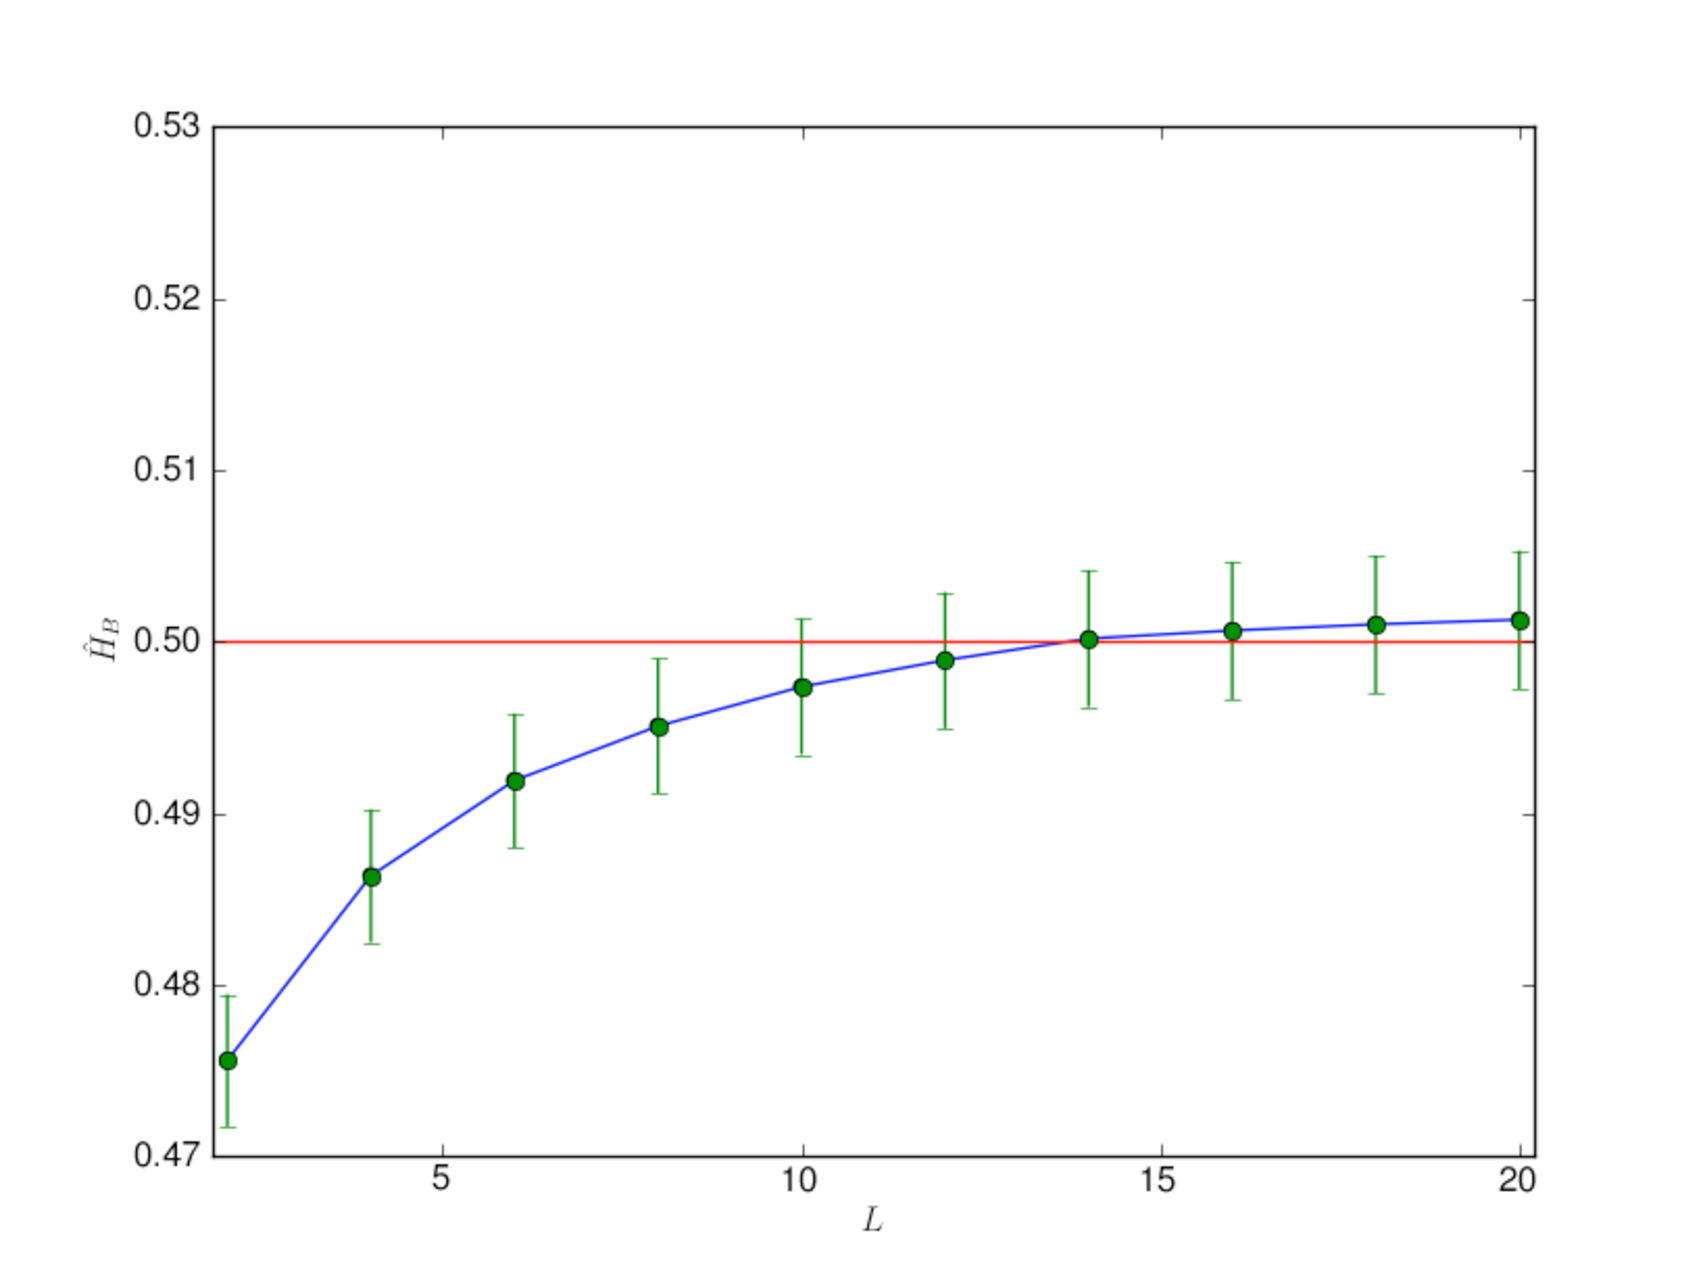
\includegraphics[scale=0.5]{Figurer/DaubEst1.pdf}
			\caption{Estimated value of the Hurst exponent based on an unbiased MODWT wavelet variance estimator 
			for Daubechies wavelets with $L = 2-20$. Maximum regression level are set according to Table 1,  	
			$J_{max}=J_{0}$. Lowest regression level, $J_{min}$, are set to 1. The errorbars marks plus/minus the
			standard deviation of the estimator. }
		\end{figure}
	\end{center}
	\begin{table}
		\begin{tabular}{| c | c | c | c | c |}
			\hline
			$L$ & $\hat{H}_{B}$ & $var\{\hat{\beta}\}$ & $SD\{\hat{H}_{B}\}$ & $t(s)$\\
		 	\hline
			2 & 0.49009 & 1.2037e-04 & 0.00549 & 0.15\\
			4 & 0.49808 & 1.2349e-04 & 0.00556 & 0.20\\
			6 & 0.50007 & 1.2588e-04 & 0.00561 & 0.25\\ 
			8 & 0.50069 & 1.2806e-04 & 0.00566 & 0.30\\
			10 & 0.50132 & 1.3003e-04 & 0.00570 & 0.33\\ 
			12 & 0.50162 & 1.3172e-04 & 0.00574 & 0.38\\ 
			14 & 0.50192 & 1.3346e-04 & 0.00578 & 0.43\\ 
			16 & 0.50123 & 1.3523e-04 & 0.00581 & 0.48\\
			18 & 0.50071 & 1.3686e-04 & 0.00585 & 0.53\\
			20 & 0.50024 & 1.3828e-04 & 0.00588 & 0.52\\ 
			\hline
		\end{tabular}
		\caption{MODWT unbiased Daubechies, Ingve's file H = 0.5, $J_{min}$=2}
	\end{table}
	\begin{center}
		\clearpage
		\begin{figure}[!h]
			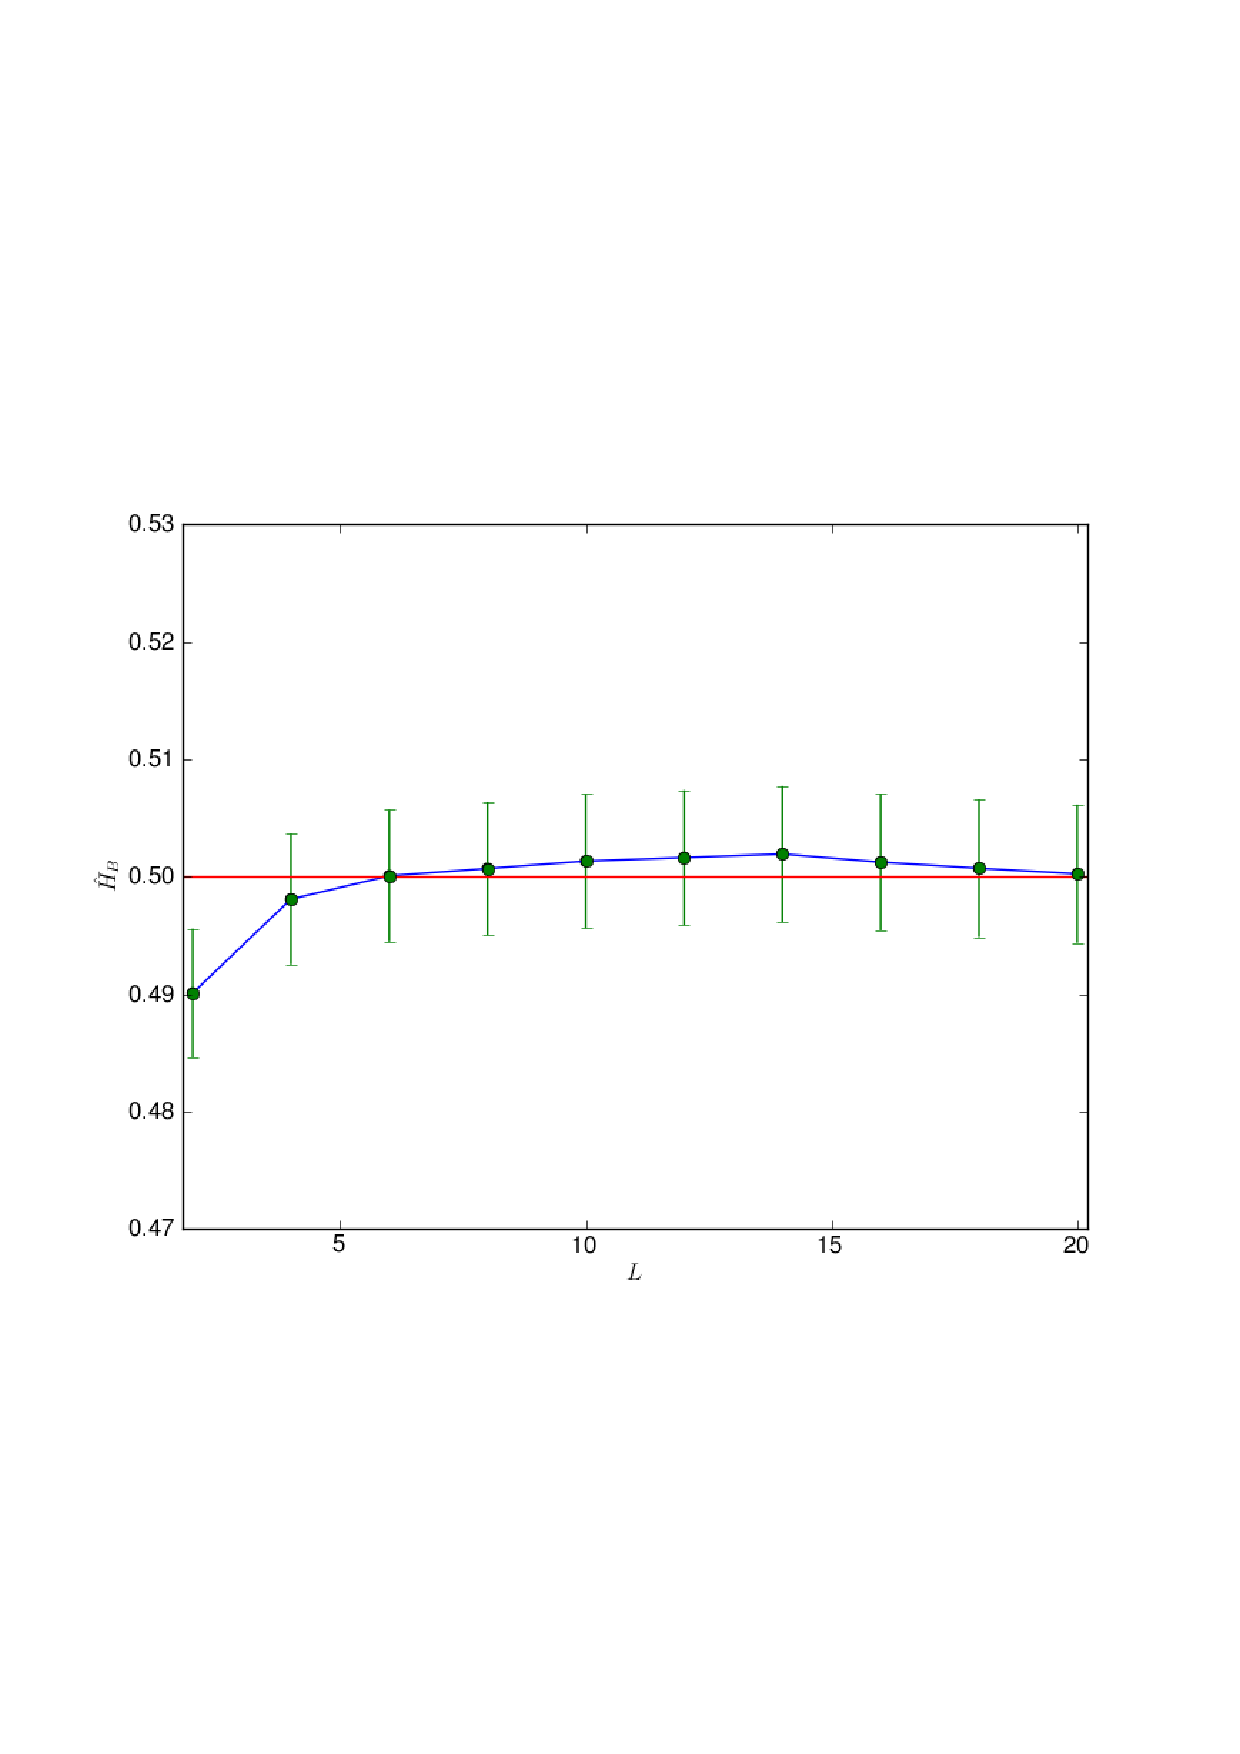
\includegraphics[scale=0.5]{Figurer/DaubEst2.pdf}
			\caption{Estimated value of the Hurst exponent based on an unbiased MODWT wavelet variance estimator 
			for Daubechies wavelets with $L = 2-20$. Maximum regression level are set according to Table 1,  	
			$J_{max}=J_{0}$. Lowest regression level, $J_{min}$, are set to 2. The errorbars marks plus/minus the
			standard deviation of the estimator. }
		\end{figure}
	\end{center}
	\begin{table}
		\begin{tabular}{| c | c | c | c | c |}
			\hline
			$L$ & $\hat{H}_{B}$ & $var\{\hat{\beta}\}$ & $SD\{\hat{H}_{B}\}$ & $t(s)$\\
		 	\hline
			2 & 0.48930 & 1.1867e-04 & 0.00545 & 0.21\\
			4 & 0.49819 & 1.1867e-04 & 0.00545 & 0.34\\
			6 & 0.50049 & 1.1867e-04 & 0.00545 & 0.48\\ 
			8 & 0.50124 & 1.1867e-04 & 0.00545 & 0.61\\
			10 & 0.50153 & 1.1867e-04 & 0.00545 & 0.76\\ 
			12 & 0.50163 & 1.1867e-04 & 0.00545 & 0.89\\ 
			14 & 0.50166 & 1.1867e-04 & 0.00545 & 1.03\\ 
			16 & 0.50166 & 1.1867e-04 & 0.00545 & 1.17\\
			18 & 0.50164 & 1.1867e-04 & 0.00545 & 1.30\\
			20 & 0.50162 & 1.1867e-04 & 0.00545 & 1.45\\ 
			\hline
		\end{tabular}
		\caption{MODWT biased reflection Daubechies, Ingve's file H = 0.5, $J_{min}$=2}
	\end{table}
	\begin{center}
		\clearpage
		\begin{figure}[!h]
			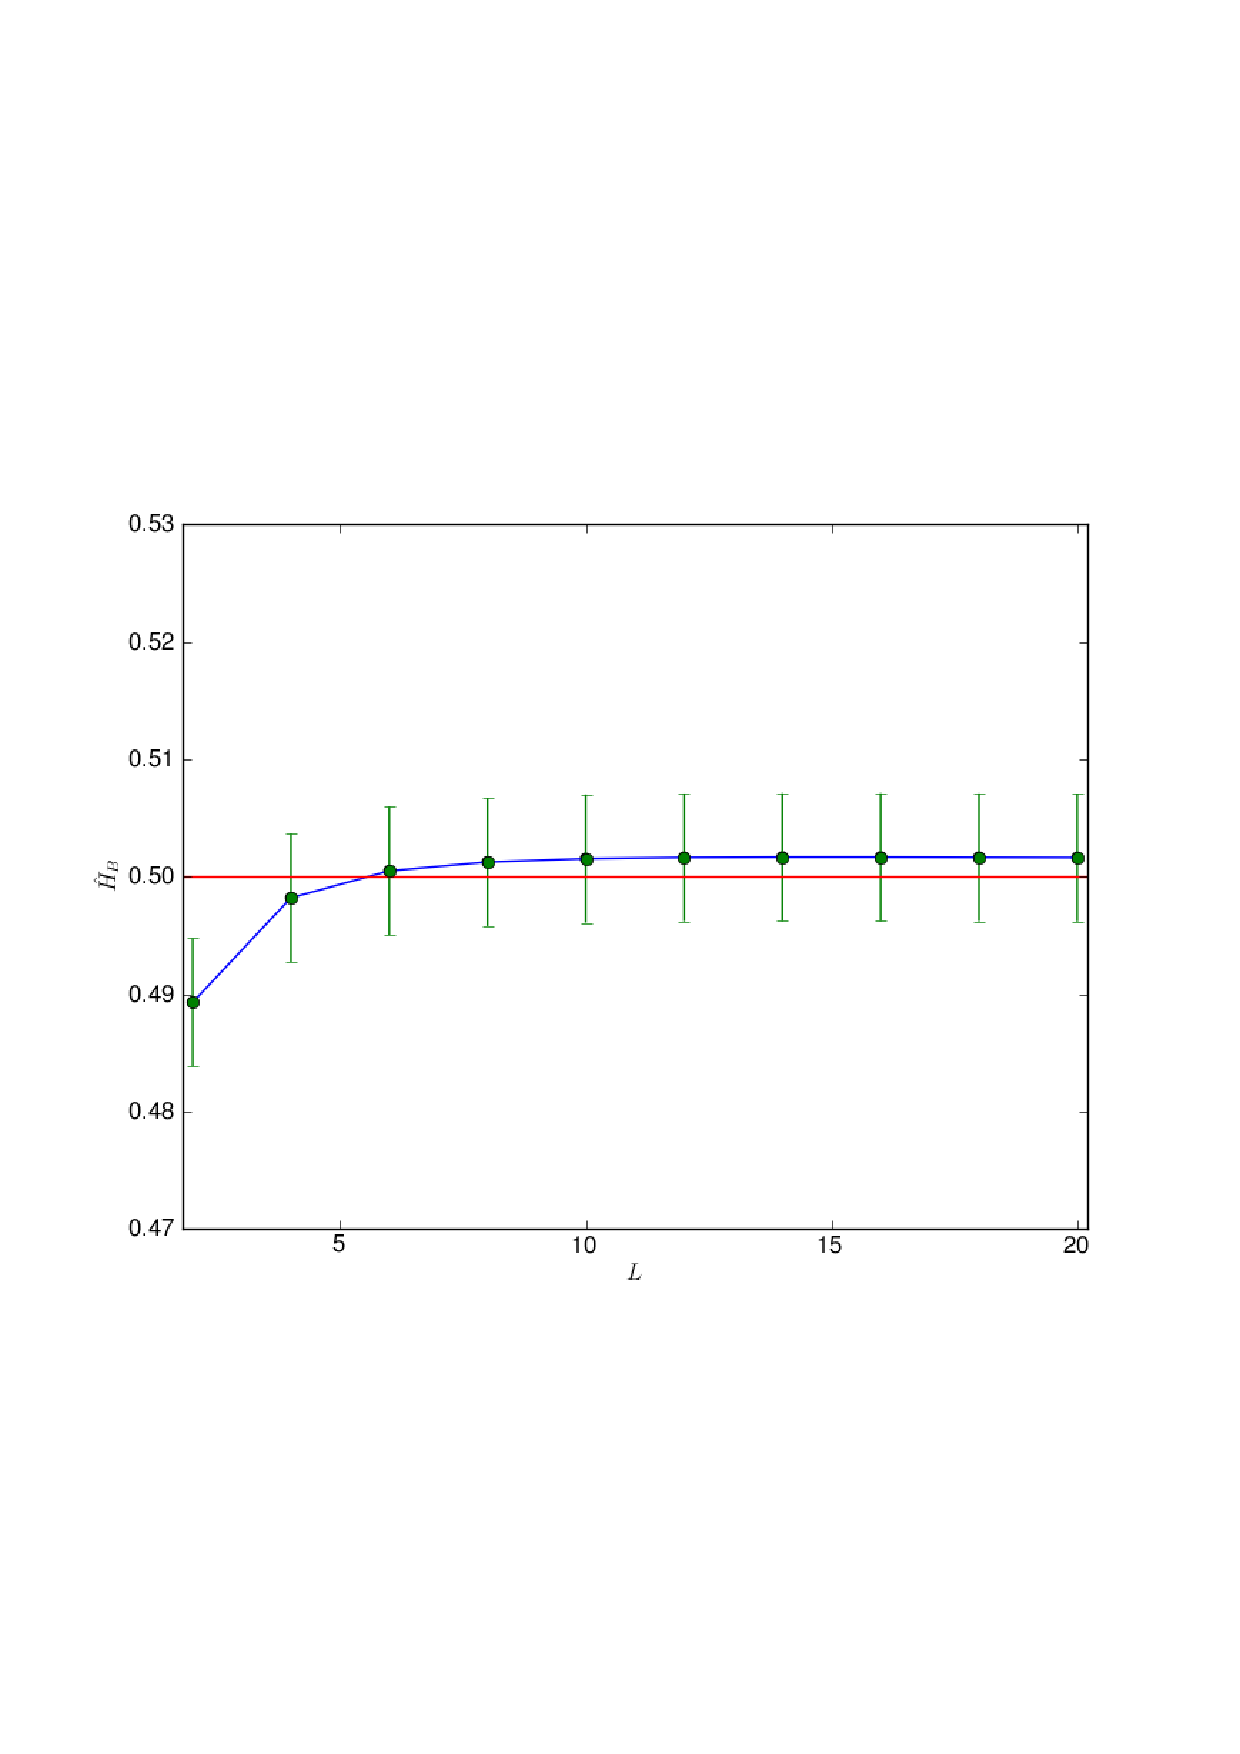
\includegraphics[scale=0.5]{Figurer/DaubEst3.pdf}
			\caption{Estimated value of the Hurst exponent based on an biased MODWT wavelet variance estimator 
			for Daubechies wavelets with $L = 2-20$ using reflection boundary conditions. Maximum regression level 
			are set according to Table 1, $J_{max}=J_{0}$. Lowest regression level, $J_{min}$, are set to 2. The 
			errorbars marks plus/minus the standard deviation of the estimator. }
		\end{figure}
	\end{center}
	
	\begin{table}
		\begin{tabular}{| c | c | c | c | c |}
			\hline
			$L$ & $\hat{H}_{B}$ & $var\{\hat{\beta}\}$ & $SD\{\hat{H}_{B}\}$ & $t(s)$\\
		 	\hline
			2 & 0.48742 & 1.1925e-04 & 0.00546 & 0.10\\
			4 & 0.49552 & 1.2264e-04 & 0.00554 & 0.11\\
			6 & 0.49854 & 1.2520e-04 & 0.00559 & 0.11\\
			8 & 0.50282 & 1.2736e-04 & 0.00564 & 0.11\\
			10 & 0.50410 & 1.2939e-04 & 0.00569 & 0.11\\
			12 & 0.49977 & 1.3107e-04 & 0.00572 & 0.11\\
			14 & 0.49871 & 1.3280e-04 & 0.00576 & 0.11\\
			16 & 0.49978 & 1.3456e-04 & 0.00580 & 0.12\\
			18 & 0.50183 & 1.3631e-04 & 0.00584 & 0.12\\
			20 & 0.50024 & 1.3772e-04 & 0.00587 & 0.12\\
			\hline
		\end{tabular}
		\caption{MODWT unbiased Daubechies, Ingve's file H = 0.5, $J_{min}$=2}
	\end{table}

	\begin{table}
		\begin{tabular}{| c | c | c | c | c |}
			\hline
			$L$ & $\hat{H}_{B}$ & $var\{\hat{\beta}\}$ & $SD\{\hat{H}_{B}\}$ & $t(s)$\\
		 	\hline
			2 & 0.48742 & 1.1925e-04 & 0.00546 & 0.10\\
			4 & 0.49552 & 1.2264e-04 & 0.00554 & 0.11\\
			6 & 0.49854 & 1.2520e-04 & 0.00559 & 0.11\\
			8 & 0.50282 & 1.2736e-04 & 0.00564 & 0.11\\
			10 & 0.50410 & 1.2939e-04 & 0.00569 & 0.11\\
			12 & 0.49977 & 1.3107e-04 & 0.00572 & 0.11\\
			14 & 0.49871 & 1.3280e-04 & 0.00576 & 0.11\\
			16 & 0.49978 & 1.3456e-04 & 0.00580 & 0.12\\
			18 & 0.50183 & 1.3631e-04 & 0.00584 & 0.12\\
			20 & 0.50024 & 1.3772e-04 & 0.00587 & 0.12\\
			\hline
		\end{tabular}
		\caption{DWT unbiased Daubechies, Ingve's file H = 0.5, $J_{min}$=2}
	\end{table}
	
	\begin{table}
		\begin{tabular}{| c | c | c | c | c |}
			\hline
			$L$ & $\hat{H}_{B}$ & $var\{\hat{\beta}\}$ & $SD\{\hat{H}_{B}\}$ & $t(s)$\\
		 	\hline
			8 & 0.49617 & 1.2736e-04 & 0.00564 & 0.11\\
			10 & 0.49966 & 1.2939e-04 & 0.00569 & 0.11\\
			12 & 0.49759 & 1.3107e-04 & 0.00572 & 0.11\\
			14 & 0.50215 & 1.3280e-04 & 0.00576 & 0.11\\
			16 & 0.49826 & 1.3456e-04 & 0.00580 & 0.12\\
			18 & 0.50233 & 1.3631e-04 & 0.00584 & 0.12\\
			20 & 0.49934 & 1.3772e-04 & 0.00587 & 0.12\\
			\hline
		\end{tabular}
		\caption{DWT unbiased Least Assymetrical, Ingve's file H = 0.5, $J_{min}$=2}
	\end{table}
	
		\begin{table}
		\begin{tabular}{| c | c | c | c | c |}
			\hline
			$L$ & $\hat{H}_{B}$ & $var\{\hat{\beta}\}$ & $SD\{\hat{H}_{B}\}$ & $t(s)$\\
		 	\hline
			14 & 0.49945 & 1.3280e-04 & 0.00576 & 0.11\\
			18 & 0.49994 & 1.3631e-04 & 0.00584 & 0.12\\
			20 & 0.50138 & 1.3772e-04 & 0.00587 & 0.12\\
			\hline
		\end{tabular}
		\caption{DWT unbiased Best Localized, Ingve's file H = 0.5, $J_{min}$=2}
	\end{table}
	
	\begin{table}
		\begin{tabular}{| c | c | c | c | c |}
			\hline
			$L$ & $\hat{H}_{B}$ & $var\{\hat{\beta}\}$ & $SD\{\hat{H}_{B}\}$ & $t(s)$\\
		 	\hline
			6 & 0.49292 & 1.2520e-04 & 0.00559 & 0.11\\
			12 & 0.49641 & 1.3107e-04 & 0.00572 & 0.11\\
			18 & 0.49778 & 1.3631e-04 & 0.00584 & 0.12\\
			24 & 0.49692 & 1.4038e-04 & 0.00592 & 0.12\\
			30 & 0.49934 & 1.4459e-04 & 0.00601 & 0.13\\
			\hline
		\end{tabular}
		\caption{DWT unbiased Coiflet, Ingve's file H = 0.5, $J_{min}$=2}
	\end{table}	
	
		
	\begin{center}
		\clearpage
		\begin{figure}[h]
			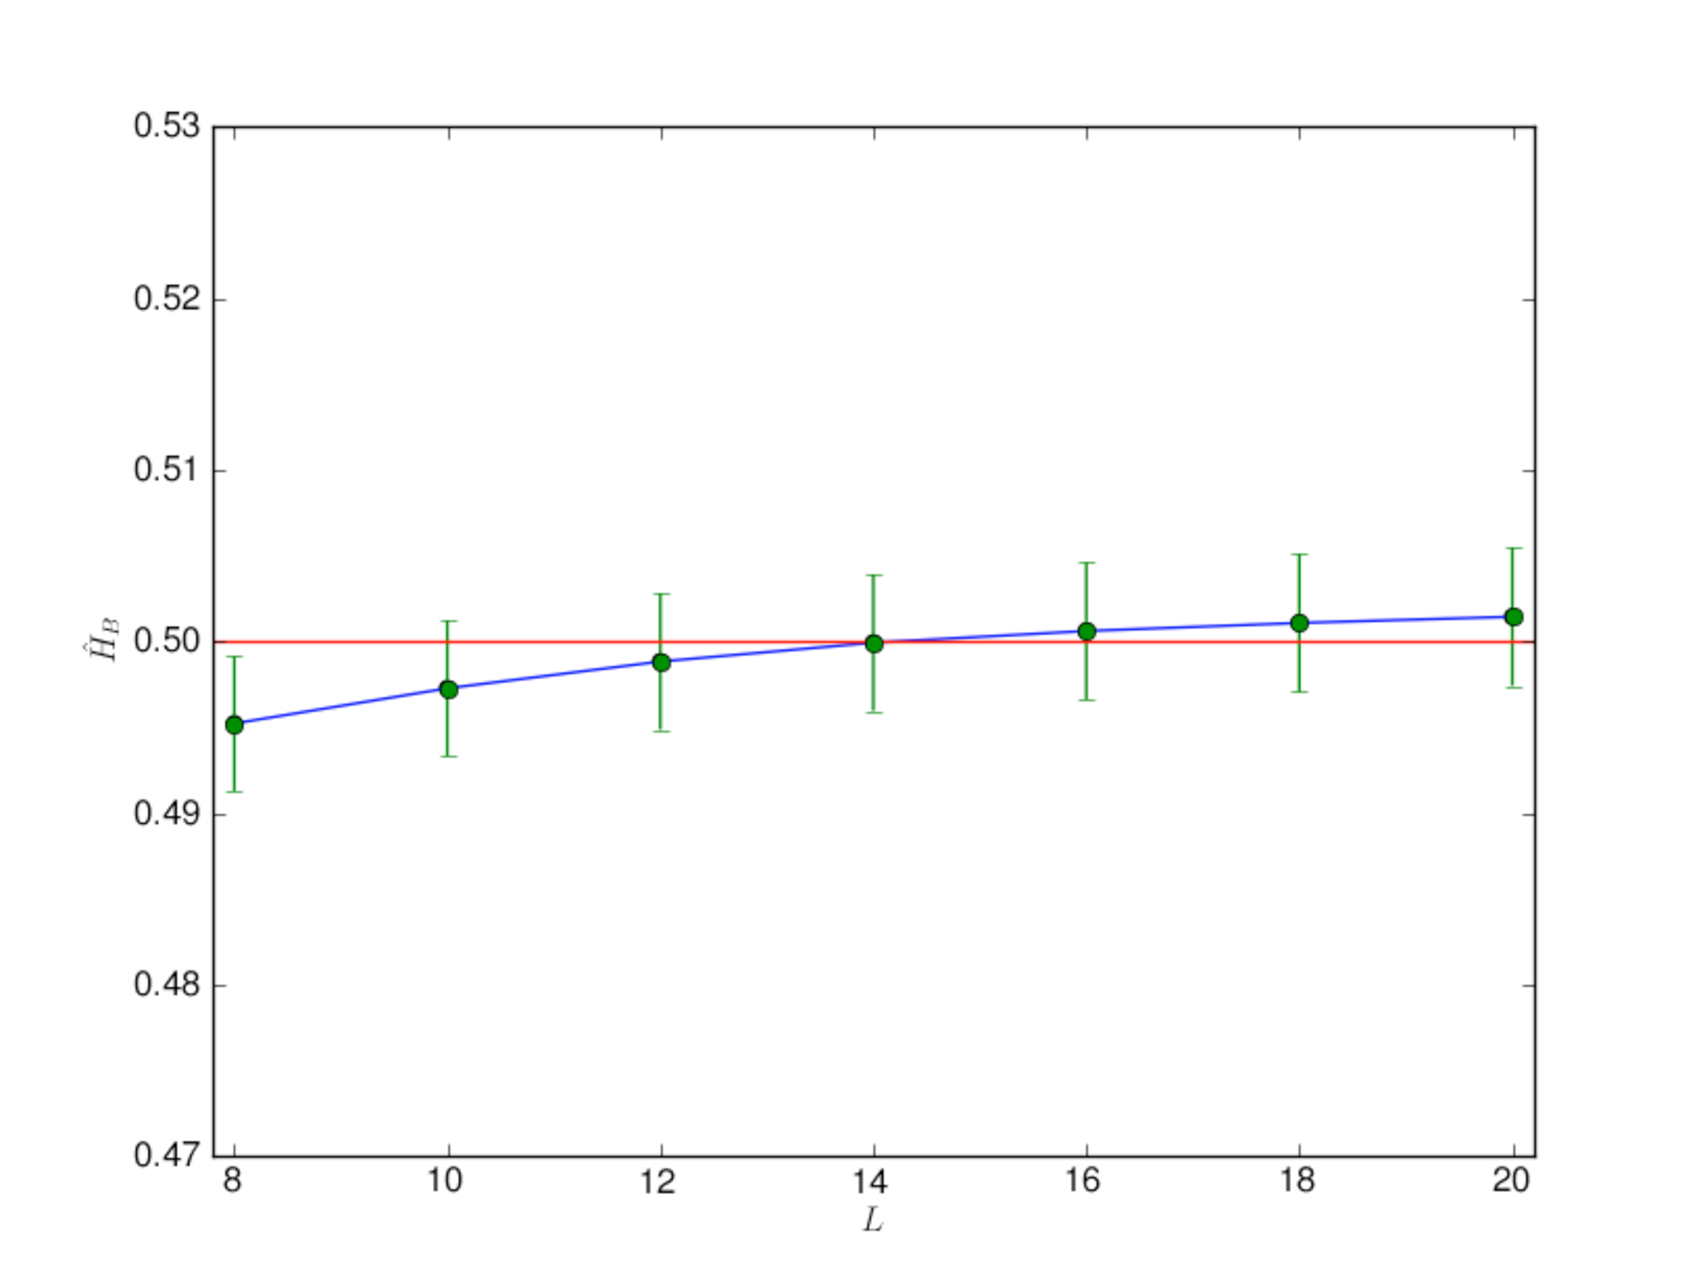
\includegraphics[scale=0.5]{Figurer/LaEst1.pdf}
			\caption{Estimated value of the Hurst exponent based on an unbiased MODWT wavelet variance estimator 
			for Least Assymetrical wavelets with $L = 8-20$. Maximum regression level are set according to Table 1,
			$J_{max}=J_{0}$. Lowest regression level, $J_{min}$, are set to 1. The errorbars marks plus/minus the
			standard deviation of the estimator. }
		\end{figure}
	\end{center}
	\begin{table}
		\begin{tabular}{| c | c | c | c | c |}
			\hline
			$L$ & $\hat{H}_{B}$ & $var\{\hat{\beta}\}$ & $SD\{\hat{H}_{B}\}$ & $t(s)$\\
		 	\hline
			8 & 0.50095 & 1.2805e-04& 0.00566 & 0.30\\
			10 & 0.50115 & 1.3003e-04& 0.00570 & 0.33\\
			12 & 0.50145 & 1.3172e-04 & 0.00574 & 0.38\\
			14 & 0.50150 & 1.3346e-04 & 0.00578 & 0.43\\
			16 & 0.50118 & 1.3523e-04 & 0.00581 & 0.48\\
			18 & 0.50080 & 1.3686e-04 & 0.00585 & 0.53\\
			20 & 0.50048 & 1.3828e-04 & 0.00588 & 0.52\\
			\hline
		\end{tabular}
		\caption{MODWT unbiased Least Assymetrical, Ingve's file H = 0.5, $J_{min}$=2}
	\end{table}	
	\begin{center}
		\clearpage
		\begin{figure}[!h]
			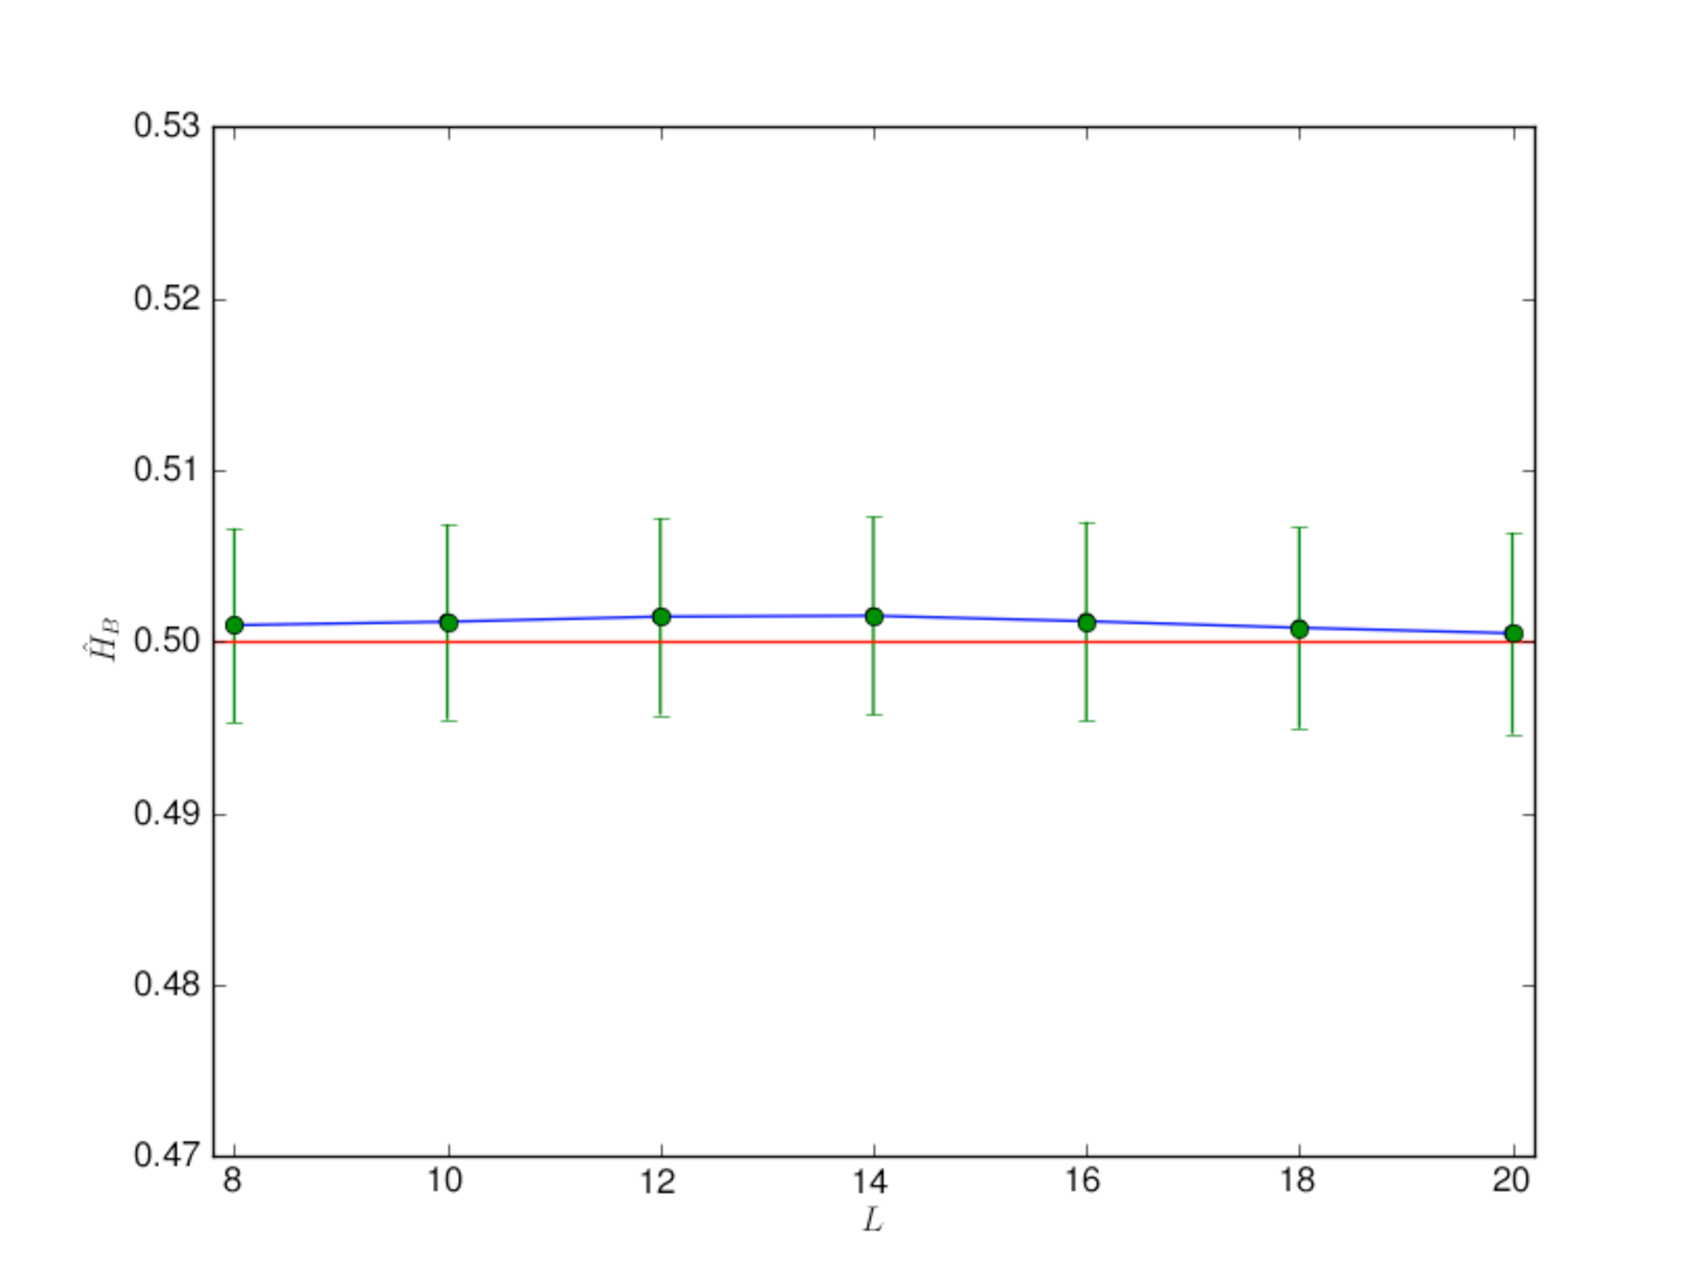
\includegraphics[scale=0.5]{Figurer/LaEst2.pdf}
			\caption{Estimated value of the Hurst exponent based on an unbiased MODWT wavelet variance estimator 
			for Least Assymetrical wavelets with $L = 8-20$. Maximum regression level are set according to Table 1,  			$J_{max}=J_{0}$. Lowest regression level, $J_{min}$, are set to 2. The errorbars marks plus/minus the          		         standard deviation of the estimator. }
		\end{figure}
	\end{center}
	\begin{table}
		\begin{tabular}{| c | c | c | c | c |}
			\hline
			$L$ & $\hat{H}_{B}$ & $var\{\hat{\beta}\}$ & $SD\{\hat{H}_{B}\}$ & $t(s)$\\
		 	\hline
			8 & 0.50125 & 1.1867e-04 & 0.00545 & 0.62\\
			10 & 0.50123 & 1.1867e-04 & 0.00545 & 0.75\\ 
			12 & 0.50163 & 1.1867e-04 & 0.00545 & 0.89\\ 
			14 & 0.50166 & 1.1867e-04 & 0.00545 & 1.03\\ 
			16 & 0.50166 & 1.1867e-04 & 0.00545 & 1.17\\
			18 & 0.50164 & 1.1867e-04 & 0.00545 & 1.31\\
			20 & 0.50162 & 1.1867e-04 & 0.00545 & 1.45\\ 
			\hline
		\end{tabular}
		\caption{MODWT biased reflection Least Assymetrical, Ingve's file H = 0.5, $J_{min}$=2}
	\end{table}
	\begin{center}
		\clearpage
		\begin{figure}[!h]
			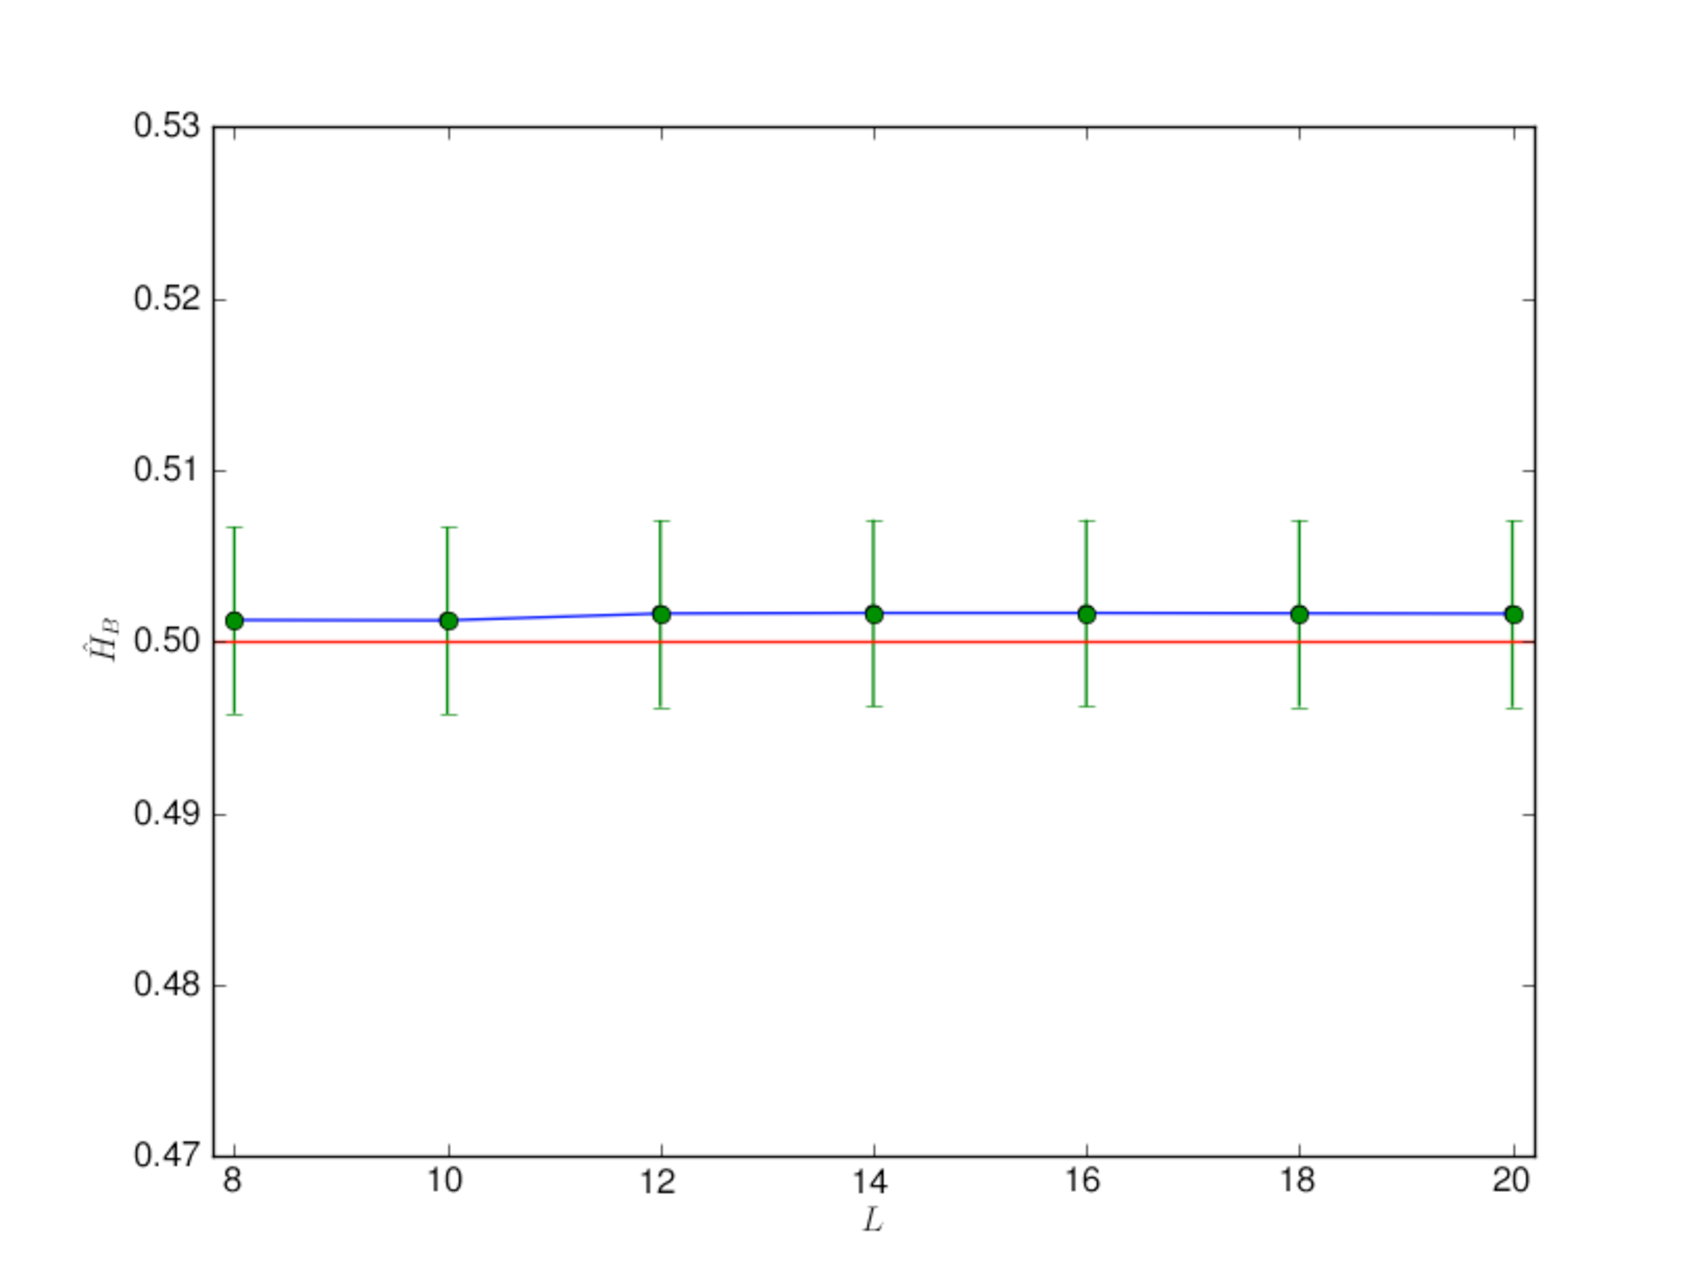
\includegraphics[scale=0.5]{Figurer/LaEst3.pdf}
			\caption{Estimated value of the Hurst exponent based on a biased MODWT wavelet variance estimator 
			for Least Assymetrical wavelets with $L = 8-20$ using reflection boundary condition. Maximum regression 
			level are set according to Table 1, $J_{max}=J_{0}$. Lowest regression level, $J_{min}$, are set to 1. The 
			errorbars marks plus/minus the standard deviation of the estimator. }
		\end{figure}
	\end{center}
	\begin{table}
		\begin{tabular}{| c | c | c | c | c |}
			\hline
			$L$ & $\hat{H}_{B}$ & $var\{\hat{\beta}\}$ & $SD\{\hat{H}_{B}\}$ & $t(s)$\\
		 	\hline
			14 & 0.50003 & 6.3491e-05 & 0.00398 & 0.43\\
			18 & 0.50099 & 6.4554e-05 & 0.00402 & 0.53\\
			20 & 0.50147 & 6.5000e-05 & 0.00403 & 0.52\\
			\hline
		\end{tabular}
		\caption{MODWT unbiased Best localized, Ingve's file H = 0.5, $J_{min}$=1}
	\end{table}	
	\begin{center}
		\clearpage
		\begin{figure}[!h]
			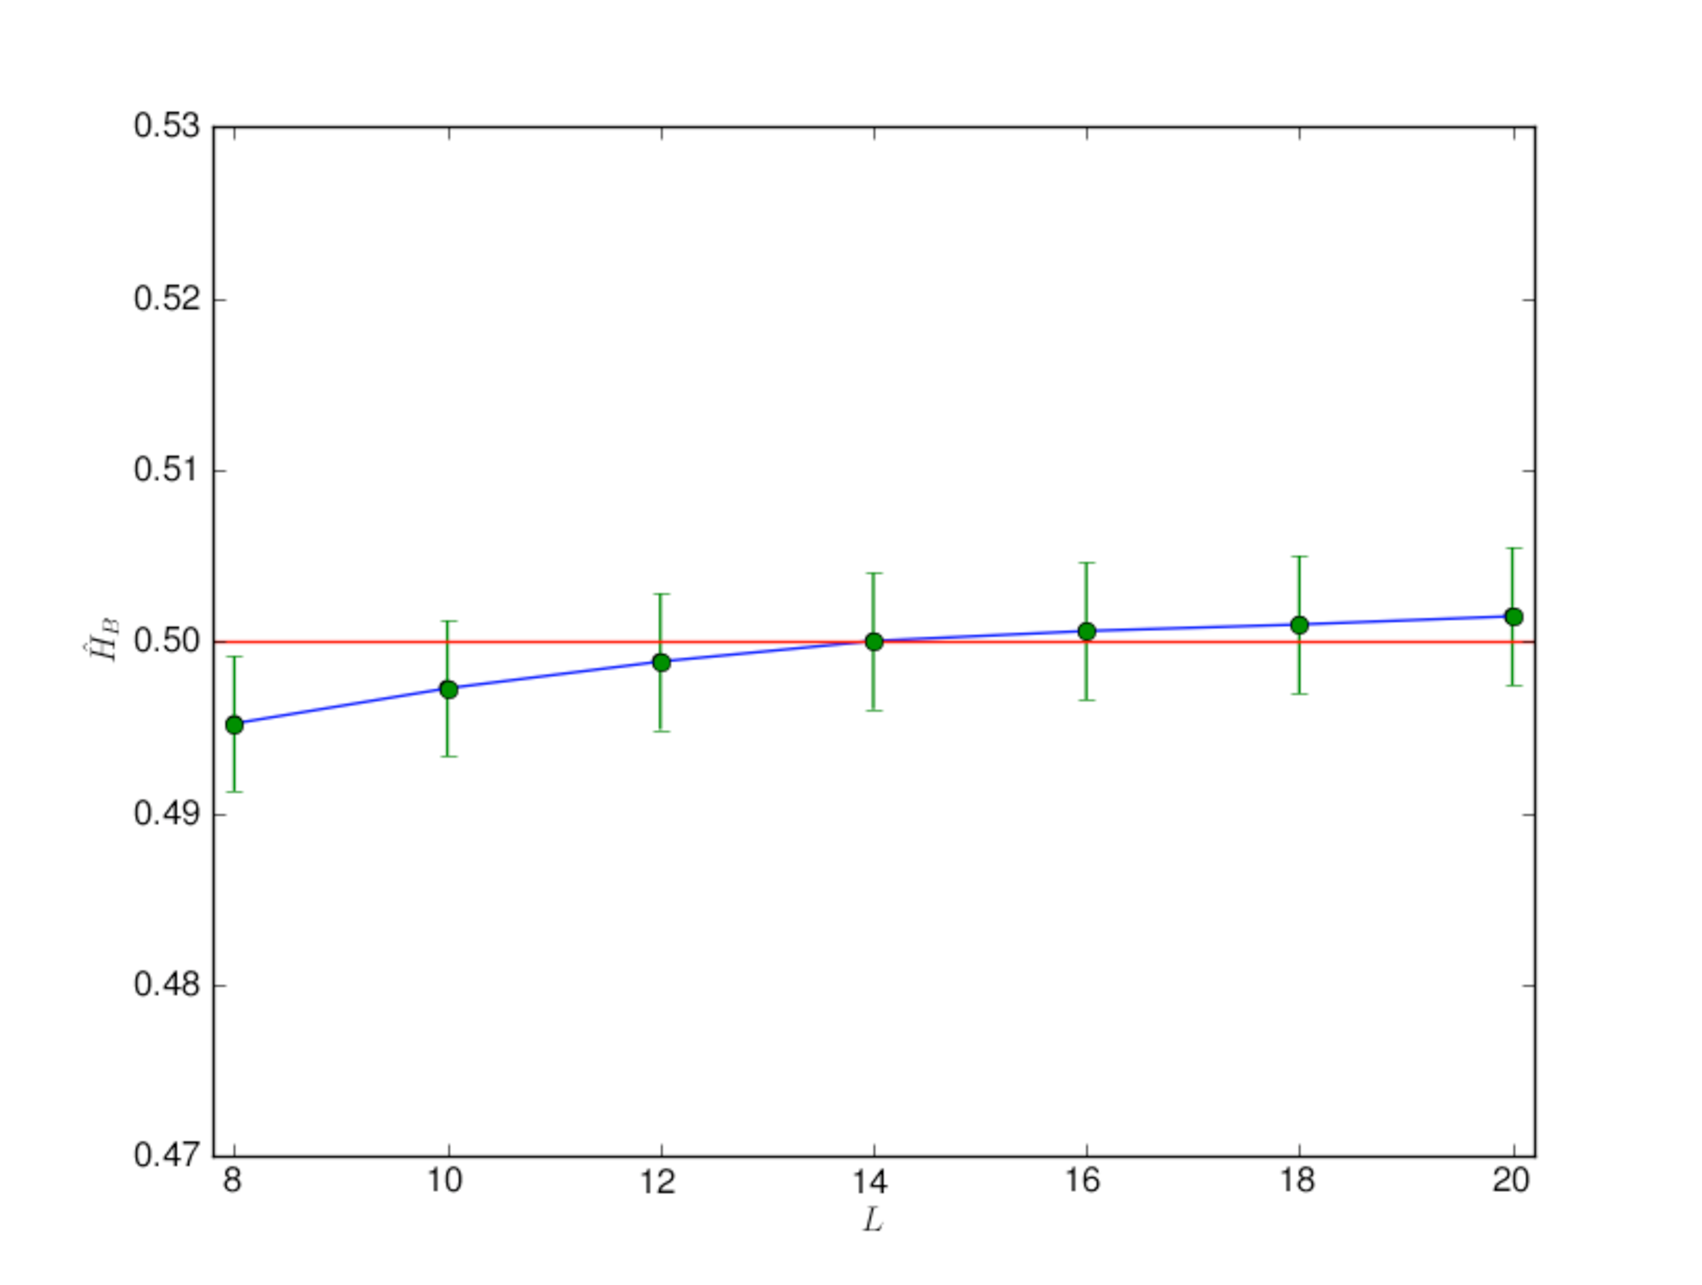
\includegraphics[scale=0.5]{Figurer/BlEst1.pdf}
			\caption{Estimated value of the Hurst exponent based on an unbiased MODWT wavelet variance estimator 
			for Best Localized wavelets with $L = 8-20$. Maximum regression level are set according to Table 1, 
			$J_{max}=J_{0}$. Lowest regression level, $J_{min}$, are set to 1. The errorbars marks plus/minus the 
			standard deviation of the estimator. }
		\end{figure}
	\end{center}
	\begin{table}
		\begin{tabular}{| c | c | c | c | c |}
			\hline
			$L$ & $\hat{H}_{B}$ & $var\{\hat{\beta}\}$ & $SD\{\hat{H}_{B}\}$ & $t(s)$\\
		 	\hline
			14 & 0.50169 & 1.3346e-04& 0.00578 & 0.43\\
			18 & 0.50066 & 1.3686e-04 & 0.00585 & 0.53\\
			20 & 0.50053 & 1.3828e-04 & 0.00588 & 0.52\\
			\hline
		\end{tabular}
		\caption{MODWT unbiased Best localized, Ingve's file H = 0.5, $J_{min}$=2}
	\end{table}
	\begin{center}
		\clearpage
		\begin{figure}[!h]
			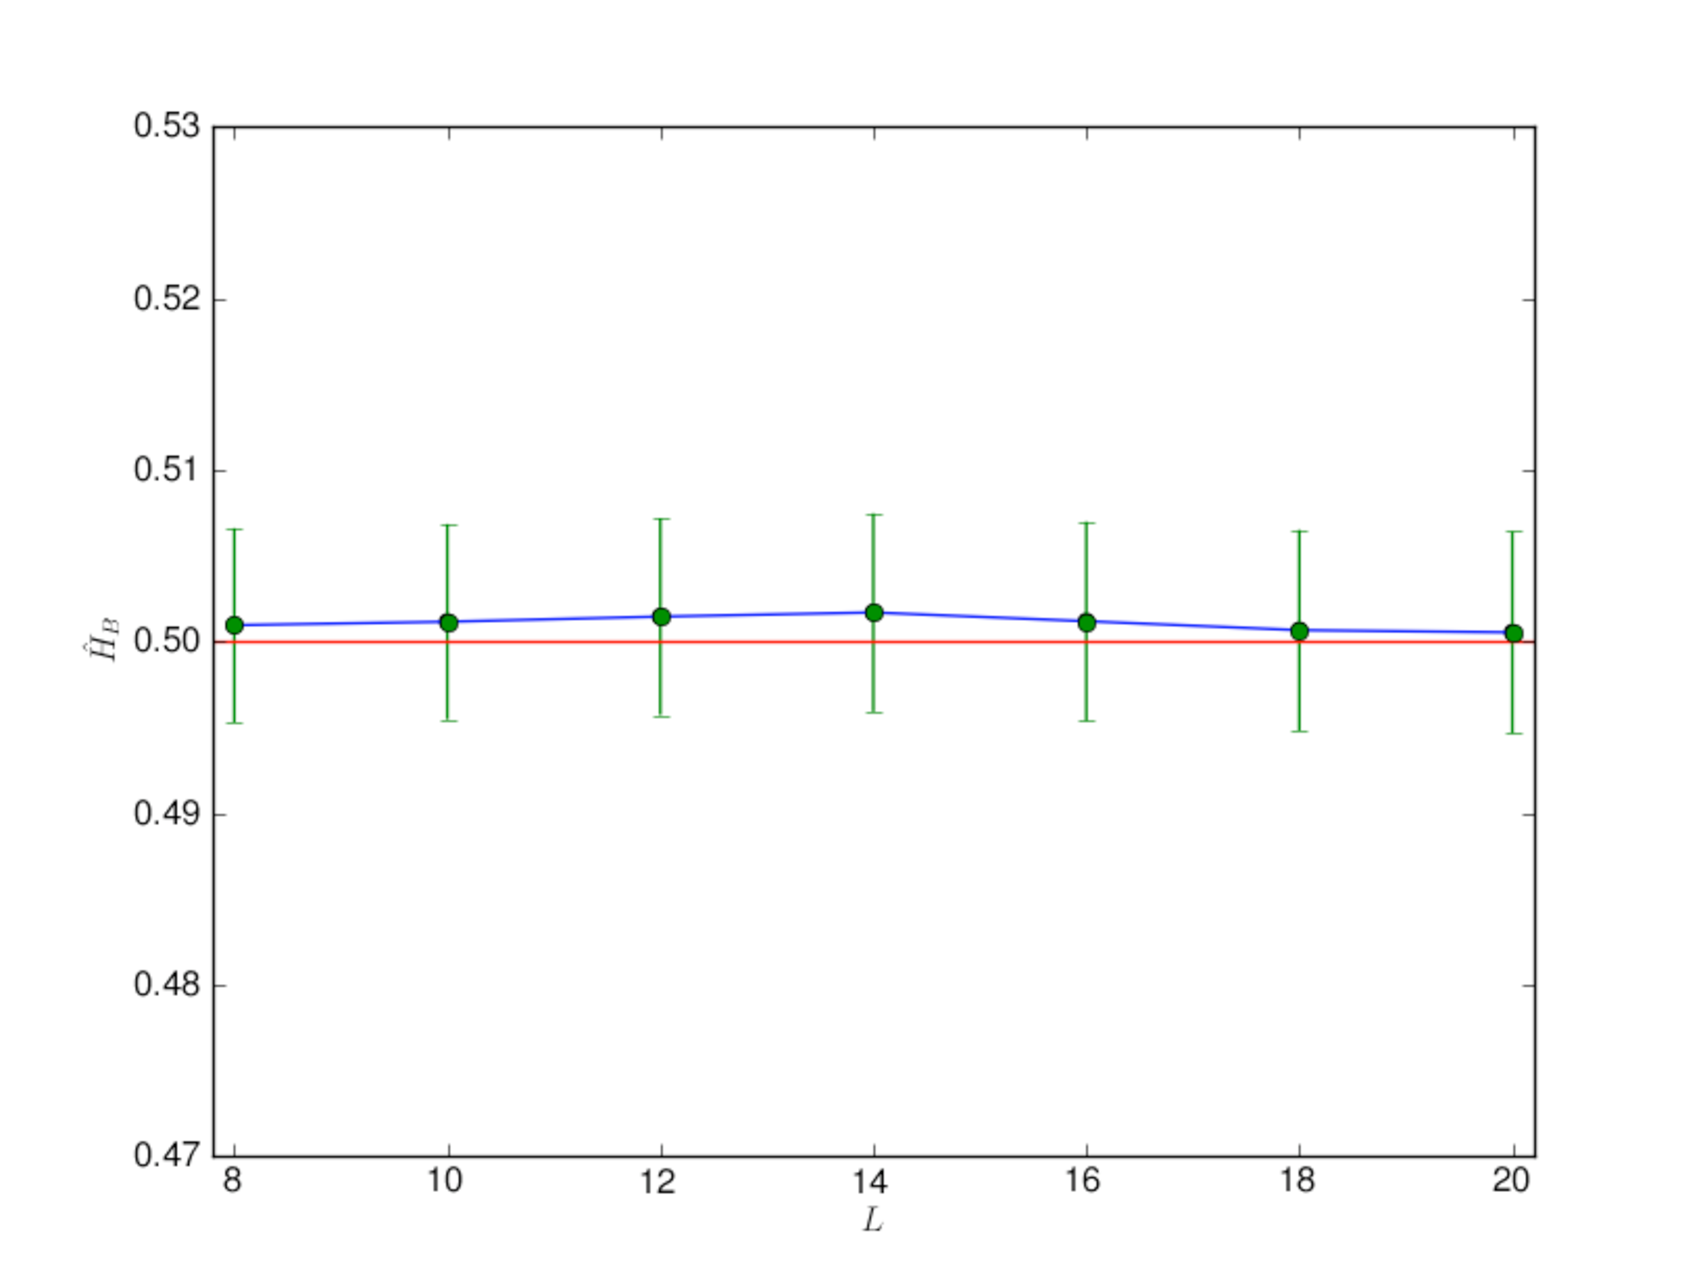
\includegraphics[scale=0.5]{Figurer/BlEst2.pdf}
			\caption{Estimated value of the Hurst exponent based on an unbiased MODWT wavelet variance estimator 
			for Best Localized wavelets with $L = 8-20$. Maximum regression level are set according to Table 1, 
			$J_{max}=J_{0}$. Lowest regression level, $J_{min}$, are set to 2. The errorbars marks plus/minus the 
			standard deviation of the estimator. }
		\end{figure}
	\end{center}
	\begin{table}
		\begin{tabular}{| c | c | c | c | c |}
			\hline
			$L$ & $\hat{H}_{B}$ & $var\{\hat{\beta}\}$ & $SD\{\hat{H}_{B}\}$ & $t(s)$\\
		 	\hline
			14 & 0.50011 & 5.8839e-05 & 0.00384 & 1.03\\
			18 & 0.50153 & 5.8839e-05  & 0.00384 & 1.31\\
			20 & 0.50204 & 5.8839e-05  & 0.00384 & 1.46\\
			\hline
		\end{tabular}
		\caption{MODWT biased reflection Best localized, Ingve's file H = 0.5, $J_{min}$=1}
	\end{table}	
	\begin{center}
		\clearpage
		\begin{figure}[!h]
			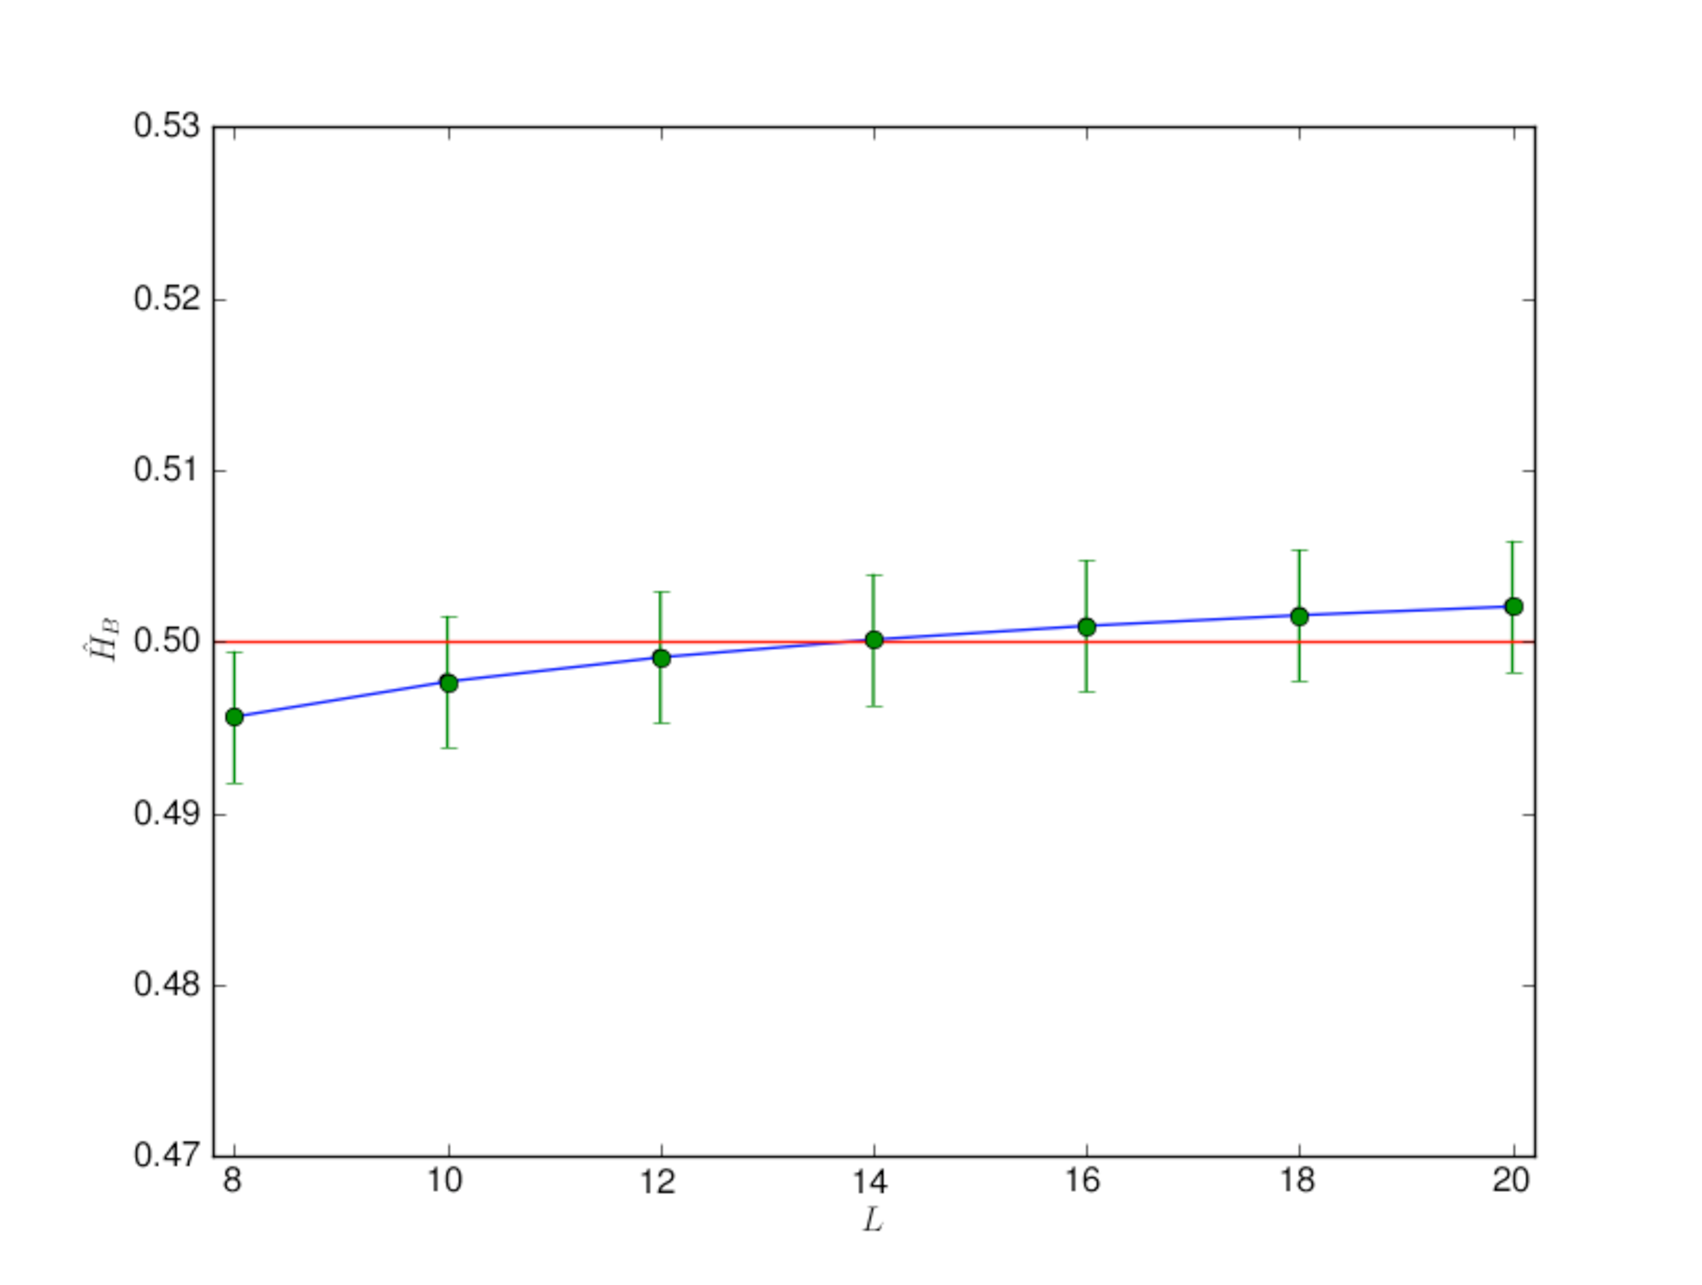
\includegraphics[scale=0.5]{Figurer/BlEst3.pdf}
			\caption{Estimated value of the Hurst exponent based on a biased MODWT wavelet variance estimator 
			for Best Localized wavelets with $L = 8-20$ using reflection boundaries. Maximum regression level are set 
			according to Table 1, $J_{max}=J_{0}$. Lowest regression level, $J_{min}$, are set to 1. The errorbars 
			marks plus/minus the standard deviation of the estimator. }
		\end{figure}
	\end{center}
	\begin{table}
		\begin{tabular}{| c | c | c | c | c |}
			\hline
			$L$ & $\hat{H}_{B}$ & $var\{\hat{\beta}\}$ & $SD\{\hat{H}_{B}\}$ & $t(s)$\\
		 	\hline
			14 & 0.50166 & 1.1867e-04 & 0.00545 & 1.03\\
			18 & 0.50164 & 1.1867e-04  & 0.00545 & 1.32\\
			20 & 0.50162 & 1.1867e-04  & 0.00545 & 1.45\\
			\hline
		\end{tabular}
		\caption{MODWT biased reflection Best localized, Ingve's file H = 0.5, $J_{min}$=2}
	\end{table}
	\begin{center}
		\clearpage
		\begin{figure}[!h]
			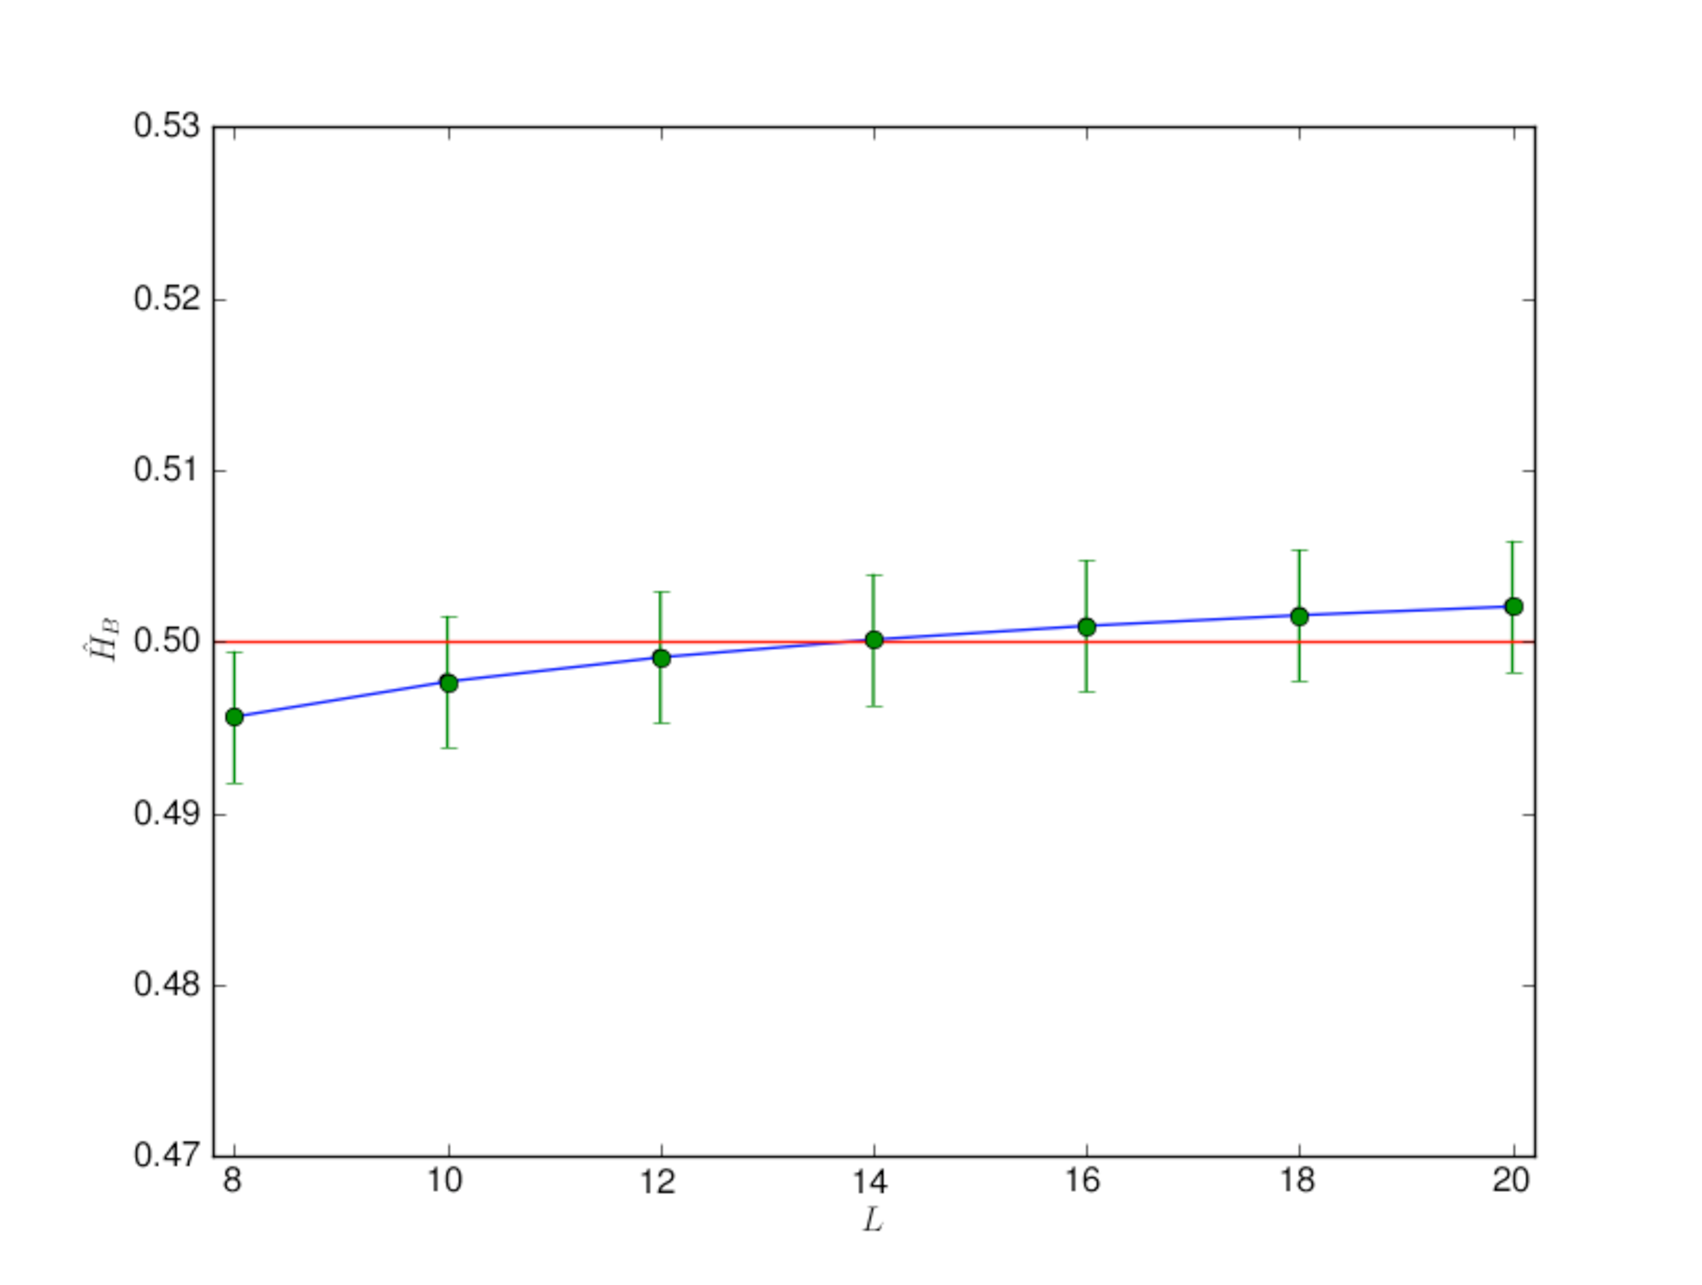
\includegraphics[scale=0.5]{Figurer/BlEst4.pdf}
			\caption{Estimated value of the Hurst exponent based on a biased MODWT wavelet variance estimator 
			for Best Localized wavelets with $L = 8-20$ using reflection boundaries. Maximum regression level are set 
			according to Table 1, $J_{max}=J_{0}$. Lowest regression level, $J_{min}$, are set to 2. The errorbars 
			marks plus/minus the standard deviation of the estimator. }
		\end{figure}
	\end{center}
	\begin{table}
		\begin{tabular}{| c | c | c | c | c |}
			\hline
			$L$ & $\hat{H}_{B}$ & $var\{\hat{\beta}\}$ & $SD\{\hat{H}_{B}\}$ & $t(s)$\\
		 	\hline
			6 & 0.48676 & 6.1099e-05 & 0.00390 & 0.25\\
			12 & 0.49576 & 6.2944e-05 & 0.00397 & 0.38\\
			18 & 0.49895 & 6.4554e-05 & 0.00402 & 0.53\\
			24 & 0.50059 & 6.5844e-05 & 0.00406 & 0.61\\
			30 & 0.50220 & 6.7152e-05 & 0.00410 & 0.74\\
			\hline
		\end{tabular}
		\caption{MODWT unbiased Coiflet, Ingve's file H = 0.5, $J_{min}$=1}
	\end{table}	
	\begin{center}
		\clearpage
		\begin{figure}[!h]
			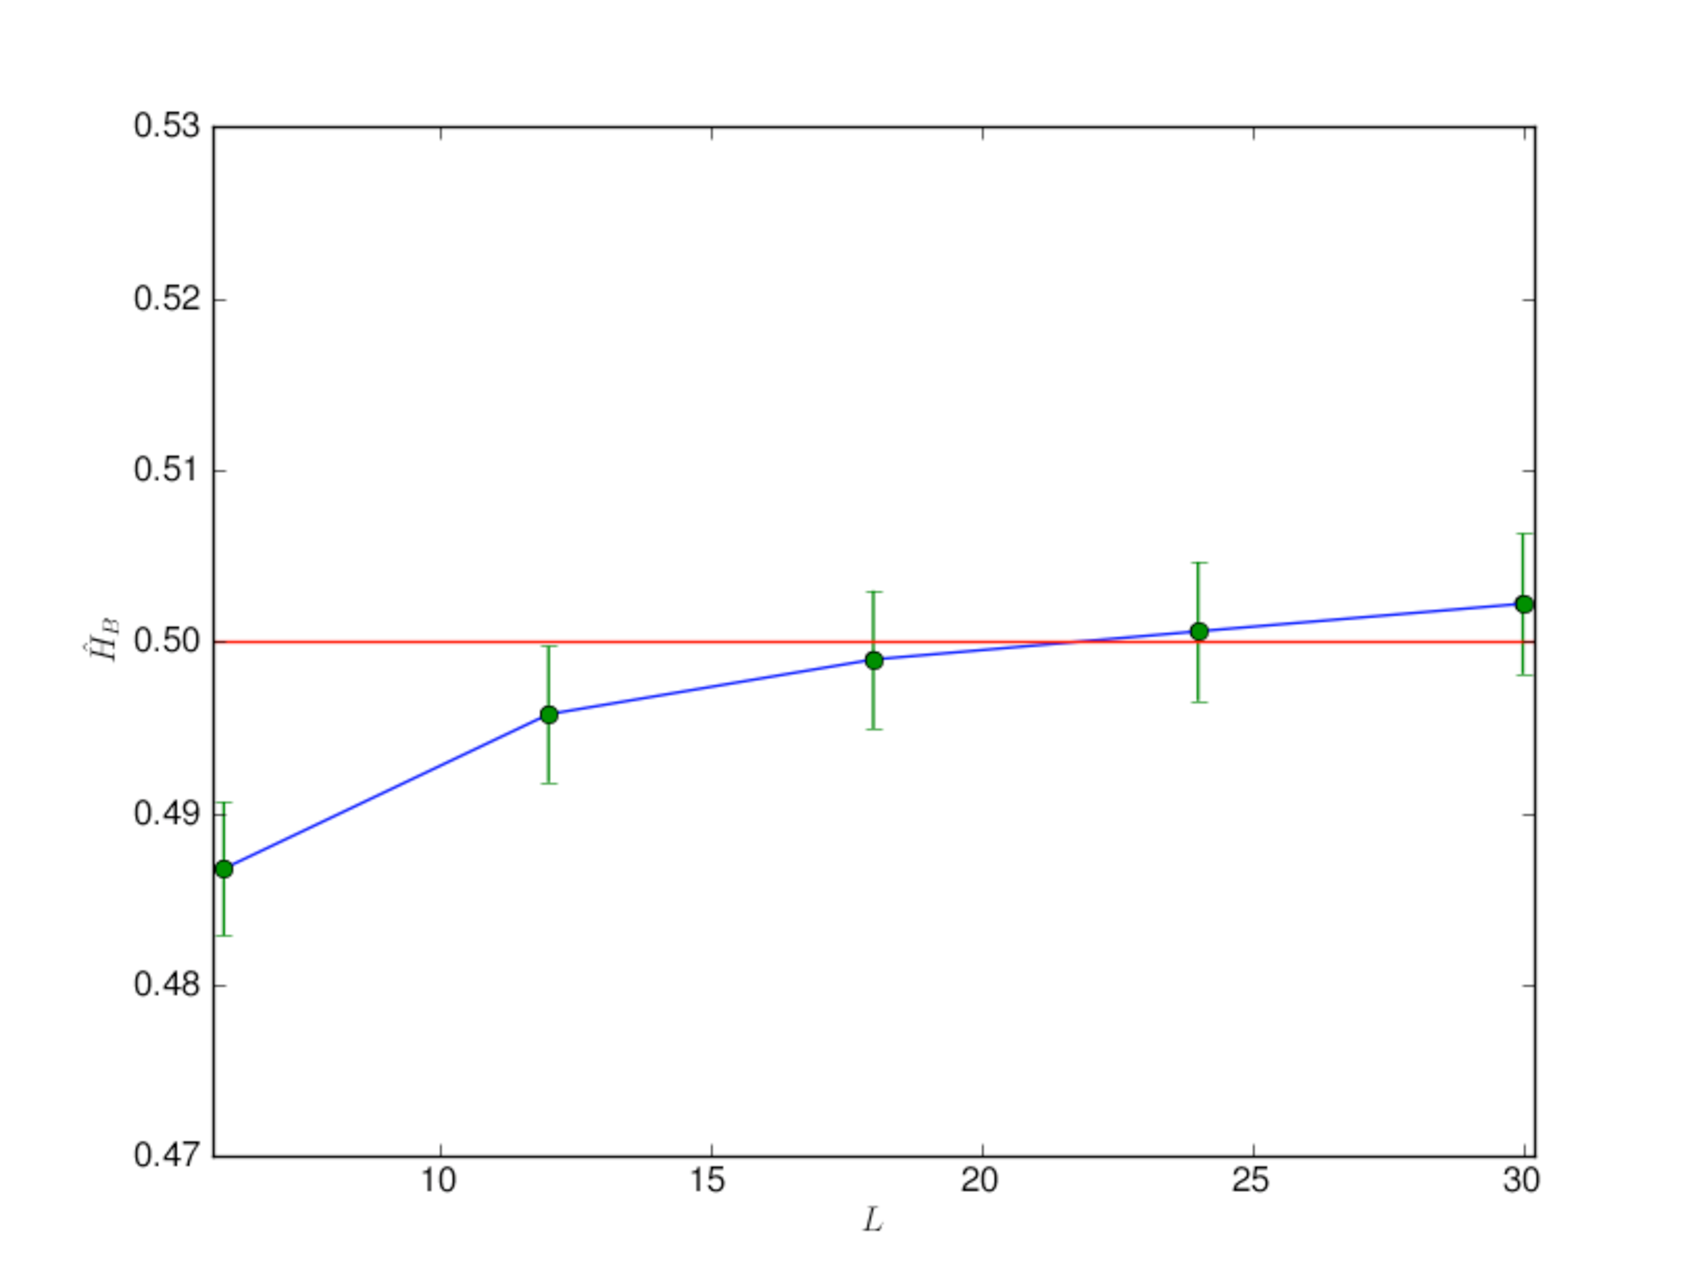
\includegraphics[scale=0.5]{Figurer/CoifEst1.pdf}
			\caption{Estimated value of the Hurst exponent based on an unbiased MODWT wavelet variance estimator 
			for Coiflet wavelets with $L = 6-30$. Maximum regression level are set 
			according to Table 1, $J_{max}=J_{0}$. Lowest regression level, $J_{min}$, are set to 1. The errorbars 
			marks plus/minus the standard deviation of the estimator. }
		\end{figure}
	\end{center}
	\begin{table}
		\begin{tabular}{| c | c | c | c | c |}
			\hline
			$L$ & $\hat{H}_{B}$ & $var\{\hat{\beta}\}$ & $SD\{\hat{H}_{B}\}$ & $t(s)$\\
		 	\hline
			6 & 0.49822 & 1.2588e-04 & 0.00561 & 0.25\\
			12 & 0.50110 & 1.3172e-04 & 0.00574 & 0.38\\
			18 & 0.50080 & 1.3686e-04 & 0.00585 & 0.53\\
			24 & 0.50054 & 1.4095e-04 & 0.00594 & 0.61\\
			30 & 0.50135 & 1.4517e-04 & 0.00602 & 0.74\\
			\hline
		\end{tabular}
		\caption{MODWT unbiased Coiflet, Ingve's file H = 0.5, $J_{min}$=2}
	\end{table}	
	\begin{center}
		\clearpage
		\begin{figure}[!h]
			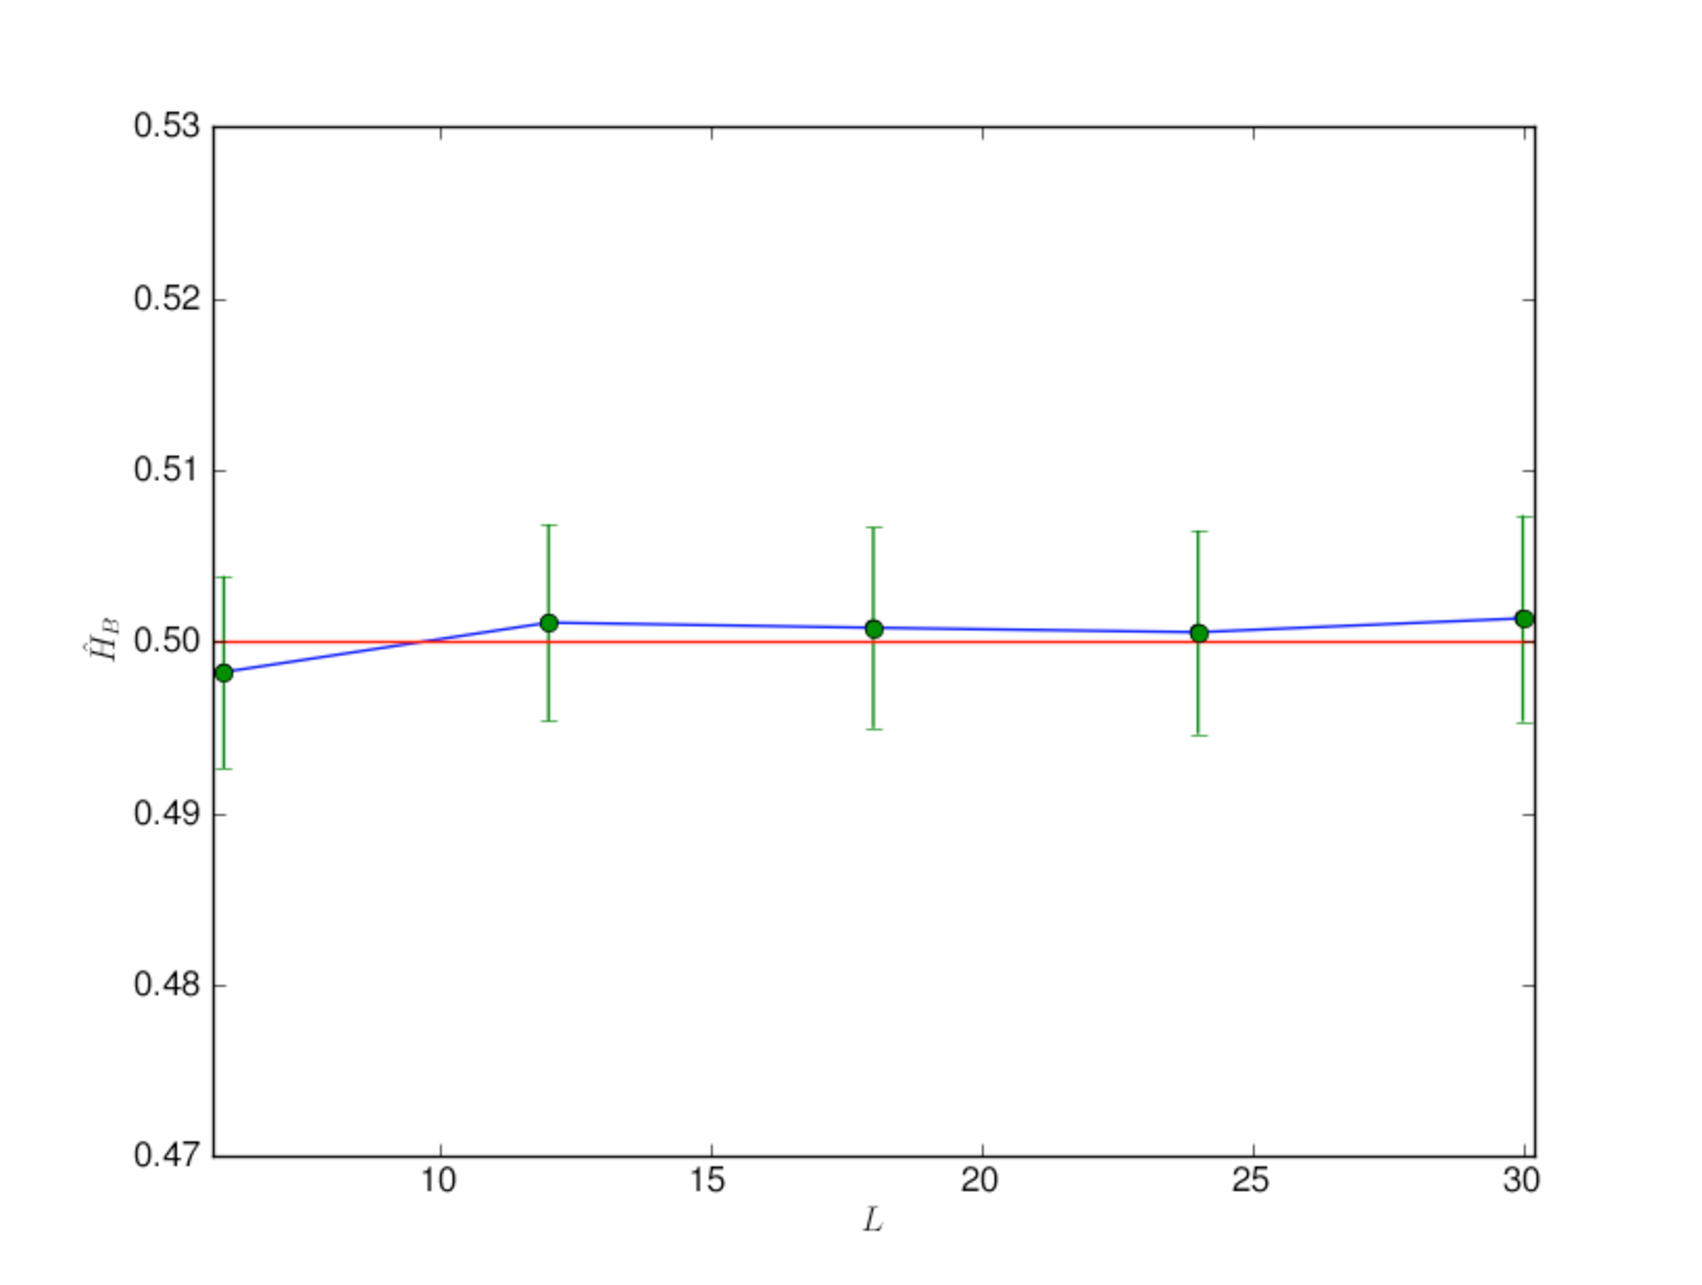
\includegraphics[scale=0.5]{Figurer/CoifEst2.pdf}
			\caption{Estimated value of the Hurst exponent based on an unbiased MODWT wavelet variance estimator 
			for Coiflet wavelets with $L = 6-30$. Maximum regression level are set 
			according to Table 1, $J_{max}=J_{0}$. Lowest regression level, $J_{min}$, are set to 2. The errorbars 
			marks plus/minus the standard deviation of the estimator. }
		\end{figure}
	\end{center}
	\begin{table}
		\begin{tabular}{| c | c | c | c | c |}
			\hline
			$L$ & $\hat{H}_{B}$ & $var\{\hat{\beta}\}$ & $SD\{\hat{H}_{B}\}$ & $t(s)$\\
		 	\hline
			6 & 0.49840 & 1.1867e-04 & 0.00545 & 0.48\\
			12 & 0.50132 & 1.1867e-04 & 0.00545 & 0.90\\
			18 & 0.50164 & 1.1867e-04 & 0.00545 & 1.31\\
			24 & 0.50164 & 1.1867e-04 & 0.00545 & 1.73\\
			30 & 0.50160 & 1.1867e-04 & 0.00545 & 2.15\\
			\hline
		\end{tabular}
		\caption{MODWT biased reflection Coiflet, Ingve's file H = 0.5, $J_{min}$=2}
	\end{table}			
	\begin{center}
		\clearpage
		\begin{figure}[!h]
			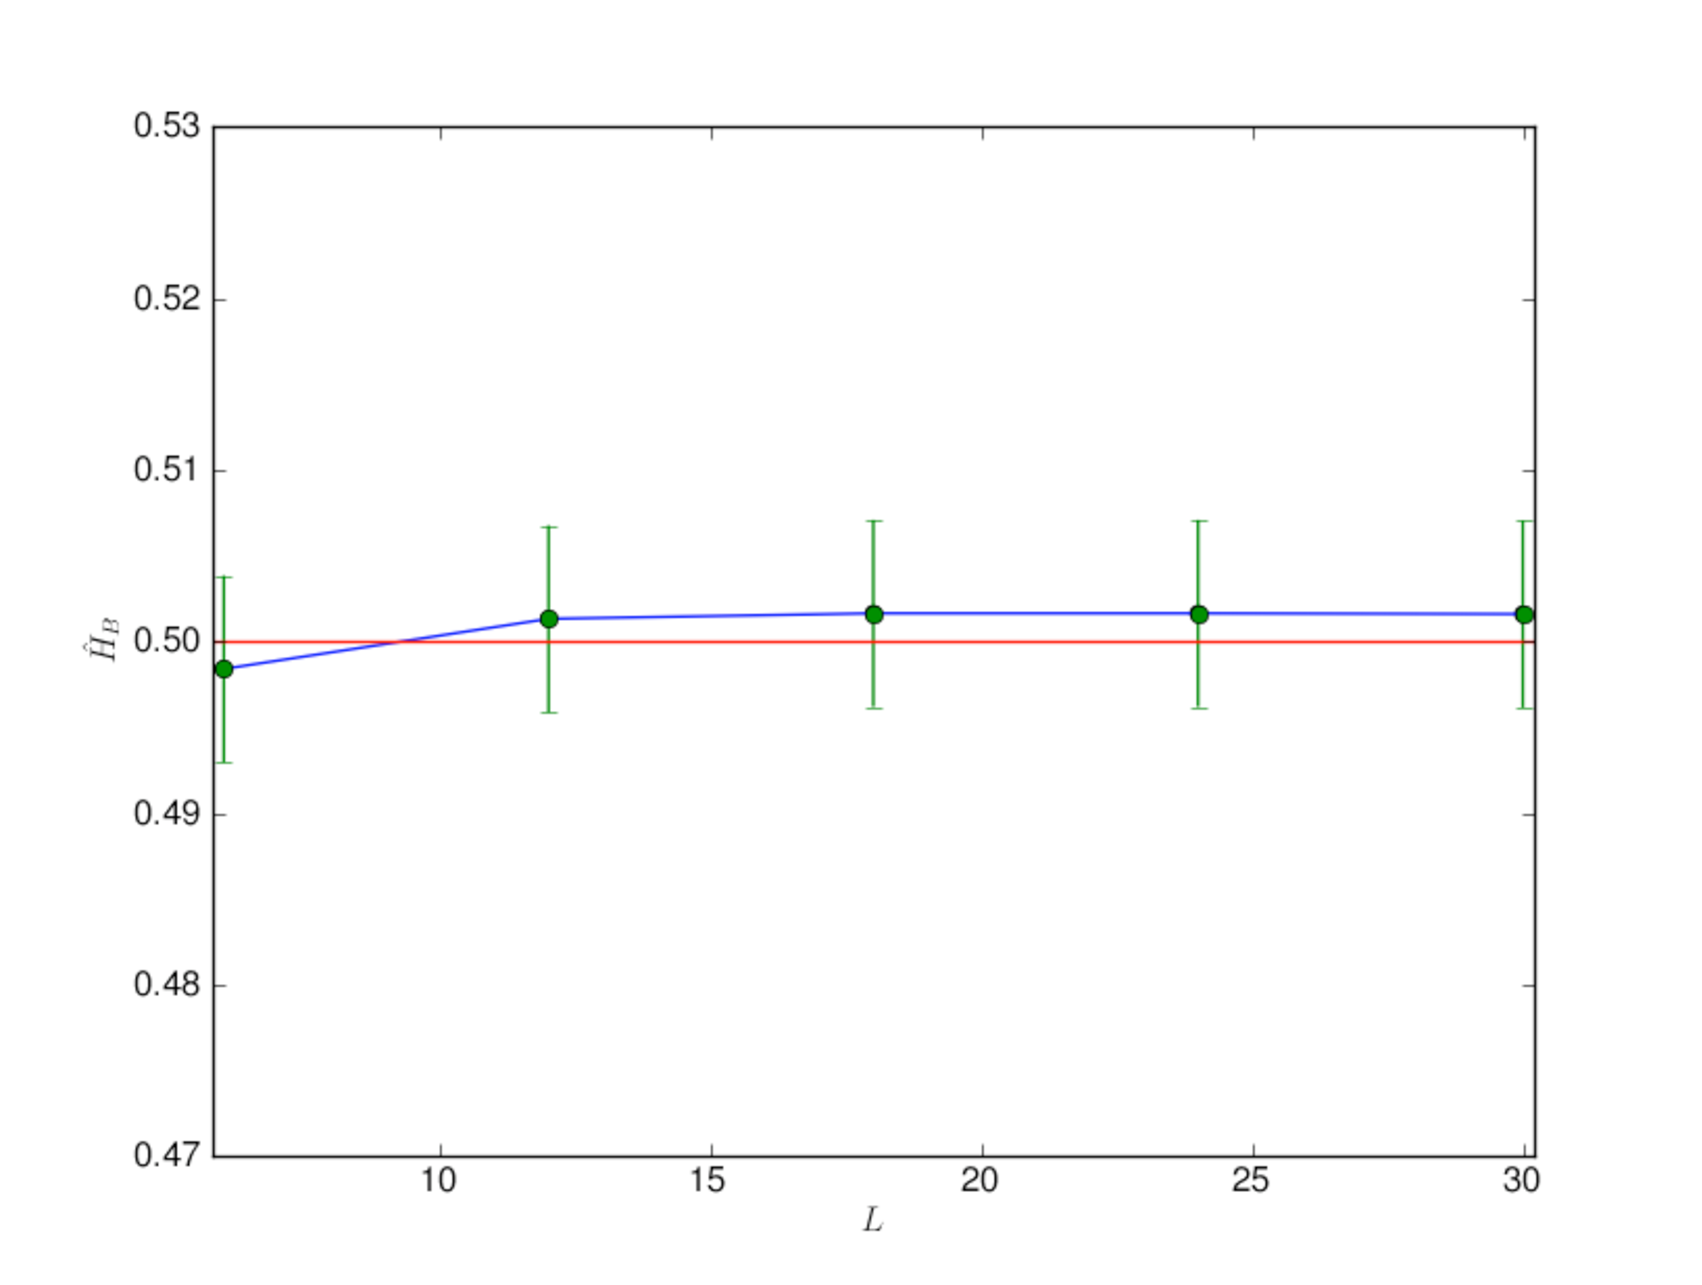
\includegraphics[scale=0.5]{Figurer/CoifEst3.pdf}
			\caption{Estimated value of the Hurst exponent based on a biased MODWT wavelet variance estimator 
			for Coiflet wavelets with $L = 6-30$ using reflection boundaries. Maximum regression level are set 
			according to Table 1, $J_{max}=J_{0}$. Lowest regression level, $J_{min}$, are set to 1. The errorbars 
			marks plus/minus the standard deviation of the estimator. }
		\end{figure}
	\end{center}
	%%%%%%%%%%%%%%%%%H = 0.7%%%%%%%%%%%%%%%%%
	\begin{table}
		\begin{tabular}{|c|c|c|c|c|c|c|c|c|c|c|c|c}
			\hline
			$L$ & $\hat{H}_{B}^{1}$ & $SD\{\hat{H}_{B}^{1}\}$ & $t^{1}(s)$
			& $\hat{H}_{B}^{2}$ & $SD\{\hat{H}_{B}^{2}\}$ & $t^{2}(s)$ 
			& $\hat{H}_{B}^{3}$ & $SD\{\hat{H}_{B}^{3}\}$ & $t^{3}(s)$
			& $\hat{H}_{B}^{4}$ & $SD\{\hat{H}_{B}^{4}\}$ & $t^{4}(s)$\\
		 	\hline
2 & 0.67908 & 0.00385 & 0.15 & 0.68876 & 0.00549 & 0.15 & 0.68770 & 0.00545 & 0.20 & 0.68672 & 0.00546 & 0.10\\
4 & 0.68689 & 0.00388 & 0.20 & 0.69839 & 0.00556 & 0.20 & 0.69836 & 0.00547 & 0.31 & 0.69570 & 0.00554 & 0.10\\
6 & 0.69177 & 0.00391 & 0.25 & 0.70009 & 0.00561 & 0.25 & 0.70014 & 0.00549 & 0.40 & 0.69733 & 0.00559 & 0.11\\
8 & 0.69483 & 0.00393 & 0.31 & 0.70067 & 0.00566 & 0.31 & 0.70085 & 0.00549 & 0.53 & 0.70276 & 0.00564 & 0.11\\
10 & 0.69712 & 0.00395 & 0.34 & 0.70130 & 0.00570 & 0.34 & 0.70091 & 0.00554 & 0.58 & 0.70451 & 0.00569 & 0.11\\
12 & 0.69869 & 0.00397 & 0.38 & 0.70159 & 0.00574 & 0.39 & 0.70106 & 0.00554 & 0.68 & 0.69961 & 0.00572 & 0.11\\
14 & 0.69998 & 0.00398 & 0.44 & 0.70189 & 0.00578 & 0.44 & 0.70114 & 0.00554 & 0.79 & 0.69812 & 0.00576 & 0.11\\
16 & 0.70051 & 0.00400 & 0.49 & 0.70124 & 0.00581 & 0.49 & 0.70119 & 0.00554 & 0.89 & 0.69986 & 0.00580 & 0.11\\
18 & 0.70090 & 0.00402 & 0.54 & 0.70073 & 0.00585 & 0.54 & 0.70121 & 0.00554 & 1.00 & 0.70271 & 0.00584 & 0.12\\
20 & 0.70120 & 0.00403 & 0.54 & 0.70028 & 0.00588 & 0.54 & 0.70235 & 0.00563 & 0.98 & 0.70054 & 0.00587 & 0.12\\
			\hline
		\end{tabular}
		\caption{1: unbiased MODWT 1-$J_0$, 2: unbiased MODWT 2-$J_0$, 3: biased, reflection MODWT 2-$J_0$, 
		4:unbiased DWT 2-$J_0$. Daubechies filter}
	\end{table}

	\begin{table}
		\begin{tabular}{|c|c|c|c|c|c|c|c|c|c|c|c|c}
			\hline
			$L$ & $\hat{H}_{B}^{1}$ & $SD\{\hat{H}_{B}^{1}\}$ & $t^{1}(s)$
			& $\hat{H}_{B}^{2}$ & $SD\{\hat{H}_{B}^{2}\}$ & $t^{2}(s)$ 
			& $\hat{H}_{B}^{3}$ & $SD\{\hat{H}_{B}^{3}\}$ & $t^{3}(s)$
			& $\hat{H}_{B}^{4}$ & $SD\{\hat{H}_{B}^{4}\}$ & $t^{4}(s)$\\
		 	\hline
8 & 0.69498 & 0.00393 & 0.31 & 0.70093 & 0.00566 & 0.31 & 0.70085 & 0.00549 & 0.53 & 0.69557 & 0.00564 & 0.11\\
10 & 0.69702 & 0.00395 & 0.34 & 0.70112 & 0.00570 & 0.34 & 0.70091 & 0.00554 & 0.58 & 0.70017 & 0.00569 & 0.11\\
12 & 0.69862 & 0.00397 & 0.39 & 0.70144 & 0.00574 & 0.39 & 0.70106 & 0.00554 & 0.68 & 0.69717 & 0.00572 & 0.11\\
14 & 0.69975 & 0.00398 & 0.44 & 0.70147 & 0.00578 & 0.44 & 0.70114 & 0.00554 & 0.79 & 0.70185 & 0.00576 & 0.11\\
16 & 0.70047 & 0.00400 & 0.49 & 0.70117 & 0.00581 & 0.49 & 0.70119 & 0.00554 & 0.89 & 0.69773 & 0.00580 & 0.12\\
18 & 0.70098 & 0.00402 & 0.54 & 0.70082 & 0.00585 & 0.54 & 0.70121 & 0.00554 & 1.00 & 0.70325 & 0.00584 & 0.12\\
20 & 0.70137 & 0.00403 & 0.54 & 0.70052 & 0.00588 & 0.54 & 0.70235 & 0.00563 & 0.98 & 0.69898 & 0.00587 & 0.12\\
			\hline
		\end{tabular}
		\caption{1: unbiased MODWT 1-$J_0$, 2: unbiased MODWT 2-$J_0$, 3: biased, reflection MODWT 2-$J_0$, 
		4:unbiased DWT 2-$J_0$. Least Assymetrical filter}
	\end{table}

	\begin{table}
		\begin{tabular}{|c|c|c|c|c|c|c|c|c|c|c|c|c}
			\hline
			$L$ & $\hat{H}_{B}^{1}$ & $SD\{\hat{H}_{B}^{1}\}$ & $t^{1}(s)$
			& $\hat{H}_{B}^{2}$ & $SD\{\hat{H}_{B}^{2}\}$ & $t^{2}(s)$ 
			& $\hat{H}_{B}^{3}$ & $SD\{\hat{H}_{B}^{3}\}$ & $t^{3}(s)$
			& $\hat{H}_{B}^{4}$ & $SD\{\hat{H}_{B}^{4}\}$ & $t^{4}(s)$\\
		 	\hline
14 & 0.69984 & 0.00398 & 0.44 & 0.70165 & 0.00578 & 0.44 & 0.70114 & 0.00554 & 0.82 & 0.69850 & 0.00576 & 0.11\\
18 & 0.70089 & 0.00402 & 0.54 & 0.70069 & 0.00585 & 0.54 & 0.70121 & 0.00554 & 0.99 & 0.69918 & 0.00584 & 0.12\\
20 & 0.70139 & 0.00403 & 0.54 & 0.70056 & 0.00588 & 0.54 & 0.70235 & 0.00563 & 0.98 & 0.70177 & 0.00587 & 0.12\\
			\hline
		\end{tabular}
		\caption{1: unbiased MODWT 1-$J_0$, 2: unbiased MODWT 2-$J_0$, 3: biased, reflection MODWT 2-$J_0$, 
		4:unbiased DWT 2-$J_0$. Best Localized filter}
	\end{table}
	
	\begin{table}
		\begin{tabular}{|c|c|c|c|c|c|c|c|c|c|c|c|c}
			\hline
			$L$ & $\hat{H}_{B}^{1}$ & $SD\{\hat{H}_{B}^{1}\}$ & $t^{1}(s)$
			& $\hat{H}_{B}^{2}$ & $SD\{\hat{H}_{B}^{2}\}$ & $t^{2}(s)$ 
			& $\hat{H}_{B}^{3}$ & $SD\{\hat{H}_{B}^{3}\}$ & $t^{3}(s)$
			& $\hat{H}_{B}^{4}$ & $SD\{\hat{H}_{B}^{4}\}$ & $t^{4}(s)$\\
		 	\hline
6 & 0.68722 & 0.00391 & 0.25 & 0.69851 & 0.00561 & 0.25 & 0.69828 & 0.00549 & 0.40 & 0.69245 & 0.00559 & 0.11\\
12 & 0.69551 & 0.00297 & 0.38 & 0.70109 & 0.00574 & 0.39 & 0.70067 & 0.00554 & 0.68 & 0.69566 & 0.00572 & 0.11\\
18 & 0.69876 & 0.00402 & 0.54 & 0.70081 & 0.00585 & 0.54 & 0.70110 & 0.00554 & 0.99 & 0.69716 & 0.00584 & 0.12\\
24 & 0.70049 & 0.00406 & 0.64 & 0.70061 & 0.00594 & 0.64 & 0.70232 & 0.00563 & 1.18 & 0.69629 & 0.00592 & 0.12\\
30 & 0.70218 & 0.00410 & 0.77 & 0.70148 & 0.00602 & 0.77 & 0.70236 & 0.00563 & 1.45 & 0.69895 & 0.00601 & 0.12\\
			\hline
		\end{tabular}
		\caption{1: unbiased MODWT 1-$J_0$, 2: unbiased MODWT 2-$J_0$, 3: biased, reflection MODWT 2-$J_0$, 
		4:unbiased DWT 2-$J_0$. Coiflet filter}
	\end{table}	
	
	%%%%%%%%%%%%%%%%%H = 0.9%%%%%%%%%%%%%%%%%
	\begin{table}
		\begin{tabular}{|c|c|c|c|c|c|c|c|c|c|c|c|c}
			\hline
			$L$ & $\hat{H}_{B}^{1}$ & $SD\{\hat{H}_{B}^{1}\}$ & $t^{1}(s)$
			& $\hat{H}_{B}^{2}$ & $SD\{\hat{H}_{B}^{2}\}$ & $t^{2}(s)$ 
			& $\hat{H}_{B}^{3}$ & $SD\{\hat{H}_{B}^{3}\}$ & $t^{3}(s)$
			& $\hat{H}_{B}^{4}$ & $SD\{\hat{H}_{B}^{4}\}$ & $t^{4}(s)$\\
		 	\hline
2 & 0.86530 & 0.00385 & 0.15 & 0.86593 & 0.00549 & 0.15 & 0.86455 & 0.00545 & 0.21 & 0.86442 & 0.00546 & 0.10\\
4 & 0.88817 & 0.00388 & 0.20 & 0.89869 & 0.00556 & 0.20 & 0.89873 & 0.00547 & 0.31 & 0.89607 & 0.00554 & 0.10\\
6 & 0.89209 & 0.00391 & 0.25 & 0.90011 & 0.00561 & 0.25 & 0.90032 & 0.00549 & 0.40 & 0.89628 & 0.00559 & 0.10\\
8 & 0.89490 & 0.00393 & 0.31 & 0.90064 & 0.00566 & 0.31 & 0.90098 & 0.00549 & 0.53 & 0.90268 & 0.00564 & 0.11\\
10 & 0.89712 & 0.00395 & 0.34 & 0.90127 & 0.00570 & 0.34 & 0.90097 & 0.00554 & 0.58 & 0.90484 & 0.00569 & 0.11\\
12 & 0.89867 & 0.00397 & 0.39 & 0.90155 & 0.00574 & 0.39 & 0.90114 & 0.00554 & 0.68 & 0.89942 & 0.00572 & 0.11\\
14 & 0.89995 & 0.00398 & 0.44 & 0.90186 & 0.00578 & 0.44 & 0.90124 & 0.00554 & 0.79 & 0.89755 & 0.00576 & 0.11\\
16 & 0.90051 & 0.00400 & 0.49 & 0.90126 & 0.00581 & 0.49 & 0.90130 & 0.00554 & 0.89 & 0.89992 & 0.00580 & 0.11\\
18 & 0.90092 & 0.00402 & 0.54 & 0.90076 & 0.00585 & 0.54 & 0.90134 & 0.00554 & 0.99 & 0.90355 & 0.00584 & 0.12\\
20 & 0.90125 & 0.00403 & 0.54 & 0.90035 & 0.00588 & 0.54 & 0.90250 & 0.00563 & 0.98 & 0.90085 & 0.00587 & 0.12\\
			\hline
		\end{tabular}
		\caption{1: unbiased MODWT 1-$J_0$, 2: unbiased MODWT 2-$J_0$, 3: biased, reflection MODWT 2-$J_0$, 
		4:unbiased DWT 2-$J_0$. Daubechies filter}
	\end{table}

	\begin{table}
		\begin{tabular}{|c|c|c|c|c|c|c|c|c|c|c|c|c}
			\hline
			$L$ & $\hat{H}_{B}^{1}$ & $SD\{\hat{H}_{B}^{1}\}$ & $t^{1}(s)$
			& $\hat{H}_{B}^{2}$ & $SD\{\hat{H}_{B}^{2}\}$ & $t^{2}(s)$ 
			& $\hat{H}_{B}^{3}$ & $SD\{\hat{H}_{B}^{3}\}$ & $t^{3}(s)$
			& $\hat{H}_{B}^{4}$ & $SD\{\hat{H}_{B}^{4}\}$ & $t^{4}(s)$\\
		 	\hline
8 & 0.89506 & 0.00393 & 0.32 & 0.90091 & 0.00566 & 0.31 & 0.90098 & 0.00549 & 0.53 & 0.89499 & 0.00564 & 0.11\\
10 & 0.89702 & 0.00395 & 0.34 & 0.90109 & 0.00570 & 0.34 & 0.90097 & 0.00554 & 0.58 & 0.90059 & 0.00569 & 0.11\\
12 & 0.89860 & 0.00397 & 0.39 & 0.90142 & 0.00574 & 0.39 & 0.90114 & 0.00554 & 0.68 & 0.89676 & 0.00572 & 0.11\\
14 & 0.89972 & 0.00398 & 0.44 & 0.90145 & 0.00578 & 0.44 & 0.90124 & 0.00554 & 0.79 & 0.90157 & 0.00576 & 0.11\\
16 & 0.90046 & 0.00400 & 0.49 & 0.90118 & 0.00581 & 0.49 & 0.90130 & 0.00554 & 0.89 & 0.89721 & 0.00580 & 0.11\\
18 & 0.90100 & 0.00402 & 0.54 & 0.90086 & 0.00585 & 0.54 & 0.90134 & 0.00554 & 0.99 & 0.90412 & 0.00584 & 0.12\\
20 & 0.90140 & 0.00403 & 0.54 & 0.90058 & 0.00588 & 0.54 & 0.90250 & 0.00563 & 0.98 & 0.89865 & 0.00587 & 0.12\\
			\hline
		\end{tabular}
		\caption{1: unbiased MODWT 1-$J_0$, 2: unbiased MODWT 2-$J_0$, 3: biased, reflection MODWT 2-$J_0$, 
		4:unbiased DWT 2-$J_0$. Least Assymetrical filter}
	\end{table}

	\begin{table}
		\begin{tabular}{|c|c|c|c|c|c|c|c|c|c|c|c|c}
			\hline
			$L$ & $\hat{H}_{B}^{1}$ & $SD\{\hat{H}_{B}^{1}\}$ & $t^{1}(s)$
			& $\hat{H}_{B}^{2}$ & $SD\{\hat{H}_{B}^{2}\}$ & $t^{2}(s)$ 
			& $\hat{H}_{B}^{3}$ & $SD\{\hat{H}_{B}^{3}\}$ & $t^{3}(s)$
			& $\hat{H}_{B}^{4}$ & $SD\{\hat{H}_{B}^{4}\}$ & $t^{4}(s)$\\
		 	\hline
14 & 0.89981 & 0.00398 & 0.44 & 0.90162 & 0.00578 & 0.44 & 0.90124 & 0.00554 & 0.79 & 0.89761 & 0.00576 & 0.11\\
18 & 0.90091 & 0.00402 & 0.54 & 0.90074 & 0.00585 & 0.54 & 0.90134 & 0.00554 & 1.00 & 0.89848 & 0.00584 & 0.12\\
20 & 0.90143 & 0.00403 & 0.54 & 0.90062 & 0.00588 & 0.54 & 0.90250 & 0.00563 & 0.98 & 0.90216 & 0.00587 & 0.12\\
			\hline
		\end{tabular}
		\caption{1: unbiased MODWT 1-$J_0$, 2: unbiased MODWT 2-$J_0$, 3: biased, reflection MODWT 2-$J_0$, 
		4:unbiased DWT 2-$J_0$. Best Localized filter}
	\end{table}

	\begin{table}
		\begin{tabular}{|c|c|c|c|c|c|c|c|c|c|c|c|c}
			\hline
			$L$ & $\hat{H}_{B}^{1}$ & $SD\{\hat{H}_{B}^{1}\}$ & $t^{1}(s)$
			& $\hat{H}_{B}^{2}$ & $SD\{\hat{H}_{B}^{2}\}$ & $t^{2}(s)$ 
			& $\hat{H}_{B}^{3}$ & $SD\{\hat{H}_{B}^{3}\}$ & $t^{3}(s)$
			& $\hat{H}_{B}^{4}$ & $SD\{\hat{H}_{B}^{4}\}$ & $t^{4}(s)$\\
		 	\hline
6 & 0.88842 & 0.00398 & 0.25 & 0.89880 & 0.00561 & 0.25 & 0.89865 & 0.00549 & 0.40 & 0.89244 & 0.00559 & 0.11\\
12 & 0.89557 & 0.00397 & 0.38 & 0.90106 & 0.00574 & 0.39 & 0.90073 & 0.00554 & 0.68 & 0.89498 & 0.00572 & 0.11\\
18 & 0.89876 & 0.00402 & 0.54 & 0.90084 & 0.00585 & 0.54 & 0.90118 & 0.00554 & 1.00 & 0.89646& 0.00584 & 0.12\\
24 & 0.90052 & 0.00406 & 0.64 & 0.90069 & 0.00594 & 0.64 & 0.90246 & 0.00563 & 1.18 & 0.89570 & 0.00592 & 0.12\\
30 & 0.90226 & 0.00410 & 0.77 & 0.90162 & 0.00602 & 0.77 & 0.90252 & 0.00563 & 1.45 & 0.89860 & 0.00601& 0.13\\
			\hline
		\end{tabular}
		\caption{1: unbiased MODWT 1-$J_0$, 2: unbiased MODWT 2-$J_0$, 3: biased, reflection MODWT 2-$J_0$, 
		4:unbiased DWT 2-$J_0$. Coiflet filter}
	\end{table}
	
	\begin{table}
		\begin{tabular}{|c|c|c|c|c|c|c|c|c|c|c|c|c}
			\hline
			$FP$ & $\hat{H}_{B}^{2}$ & $SD\{\hat{H}_{B}^{2}\}$ & $Range$ 
			& $\hat{H}_{B}^{3}$ & $SD\{\hat{H}_{B}^{3}\}$ & $Range$
			& $\hat{H}_{B}^{4}$ & $SD\{\hat{H}_{B}^{4}\}$ & $Range$\\
		 	\hline
1 & 0.65 & 0.07 & 2-6 & 0.72 & 0.05 & 2-9 & 0.82 & 0.07 & 2-6\\
2 & 0.26 & 0.07 & 1-5 & 0.65 & 0.07 & 3-9 & 0.35 & 0.04 & 1-6\\
3 & 0.92 & 0.04 & 1-6 & 0.81 & 0.05 & 2-9 & 0.88 & 0.04 & 1-6\\
4 & 0.64 & 0.07 & 2-6 & 0.55 & 0.05 & 2-9 & 0.58 & 0.07 & 2-6\\
5 & 0.89*& 0.11* & 4-6 & 0.975* & 0.0025* & 3-9 & 0.37 & 0.07 & 2-6\\
6 & 0.54 & 0.07 & 2-6 & 0.56 & 0.05 & 2-9 & 0.61 & 0.07 & 2-6\\
7 & 0.79 & 0.07 & 2-6 & 0.70 & 0.05 & 2-9 & 0.83 & 0.07 & 2-6\\
8 & 0.65 & 0.07 & 2-6 & 0.75 & 0.05 & 2-9 & 0.67 & 0.07 & 2-6\\
9 & 0.49 & 0.07 & 2-6 & 0.46 & 0.05 & 2-9 & 0.41 & 0.07 & 2-6\\
10 & 0.09 & 0.07 & 2-6 & 0.19 & 0.05 & 2-9 & 0.01 & 0.07 & 2-6\\
11 & 0.72 & 0.07 & 2-6 & 0.62 & 0.05 & 2-9 & 0.80 & 0.07 & 2-6\\
12 & 0.21 & 0.05 & 1-6 & 0.22** & 0.05 & 2-9 & 0.20 & 0.04 & 1-6\\ %Clear that the unbiased algos do not "see" the lows 
13 & 0.22 & 0.07 & 2-6 & 0.26 & 0.05 & 2-9 & 0.18 & 0.07 & 2-6\\
14 & 0.45 & 0.12 & 3-6 & 0.81*** & 0.05 & 2-9 & 0.90 & 0.23 & 4-6\\
15 & 0.40 & 0.07 & 2-6 & 0.39 & 0.05 & 2-9 & 0.39 & 0.07 & 2-6\\
16 & 0.14 & 0.07 & 2-6 & 0.87 & 0.11 & 4-9 & 0.17 & 0.07 & 2-6\\ %See only the start of the time series...
17 & 0.33 & 0.07 & 2-6 & 0.23 & 0.05 & 2-9 & 0.33 & 0.07 & 2-6\\
			\hline
		\end{tabular}
		\caption{2: unbiased MODWT $J_0$=6, 3: biased, reflection MODWT $J_0$=9, 
		4:unbiased DWT $J_0$=6. D6 wavelet
		*v1: 1.02 +/- 0.24, v2: 1.02 +/-0.07
		**Range 5-9 yields 0.88 +/-0.19
		***Range 4-9 yields 0.99 +/- 0.11}
	\end{table}

	\begin{table}
		\begin{tabular}{|c|c|c|c|c|c|c|c|c|c|c|c|c}
			\hline
			$FP$ & $\hat{H}_{B}^{2}$ & $SD\{\hat{H}_{B}^{2}\}$ & $Range$ 
			& $\hat{H}_{B}^{3}$ & $SD\{\hat{H}_{B}^{3}\}$ & $Range$
			& $\hat{H}_{B}^{4}$ & $SD\{\hat{H}_{B}^{4}\}$ & $Range$\\
		 	\hline
1 & 0.53 & 0.07 & 2-6 & 0.58 & 0.05 & 2-9 & 0.58 & 0.04 & 1-6\\
2 & 0.36 & 0.04 & 1-6 & 0.43 & 0.05 & 2-9 & 0.39 & 0.04 & 1-6\\
3 & 0.66 & 0.05 & 1-5 & 0.59 & 0.05 & 2-9 & 0.68 & 0.04 & 1-5\\
4 & 0.51 & 0.07 & 2-6 & 0.49 & 0.05 & 2-9 & 0.54 & 0.04 & 1-5\\
5 & 0.12 & 0.07 & 2-6 & 0.11 & 0.05 & 2-9 & 0.09 & 0.07 & 2-6\\
6 & 0.09 & 0.07 & 2-6 & 0.45 & 0.05 & 2-9 & 0.02 & 0.07 & 2-6\\
7 & 0.78 & 0.07 & 2-6 & 0.68 & 0.05 & 2-9 & 0.79 & 0.04 & 1-6\\
8 & 0.49 & 0.07 & 2-6 & 0.50 & 0.05 & 2-9 & 0.51 & 0.04 & 1-6\\
9 & 0.14 & 0.07 & 2-6 & 0.27 & 0.06 & 2-6 & 0.15 & 0.07 & 2-6\\
10& 0.42 & 0.04 & 1-6 & 0.54 & 0.05 & 2-9 & 0.42 & 0.04 & 1-6\\
11& 0.81 & 0.07 & 2-6 & 0.63 & 0.05 & 2-9 & 0.81 & 0.07 & 2-6\\
12 & 0.30 & 0.07 & 2-6 & 0.38 & 0.05 & 2-9 & 0.35 & 0.07& 2-6\\
13 & 0.21 & 0.07 & 2-6 & 0.14 & 0.05 & 2-9 & 0.19 & 0.07 & 2-6\\
14 & 0.69 & 0.07 & 2-6 & 0.72 & 0.05 & 2-9 & 0.66 & 0.07 & 2-6\\
15 & 0.28 & 0.07 & 2-6 & 0.40 & 0.05 & 2-9 & 0.27 & 0.07 & 2-6\\
16 & 0.04 & 0.04 & 1-6 & 0.10 & 0.05 & 2-9 & 0.01 & 0.04 & 1-6\\
17 & 0.27 & 0.07 & 2-6 & 0.23 & 0.05 & 2-9 & 0.28 & 0.07 & 2-6\\
			\hline
		\end{tabular}
		\caption{2: unbiased MODWT $J_0$=6, 3: biased, reflection MODWT $J_0$=9, 
		4:unbiased DWT $J_0$=6. D6 wavelet}
	\end{table}
	
	\begin{table}
		\begin{tabular}{|c|c|c|c|c|c|c|c|c|c|c|c|c}
			\hline
			$FP$ & $\hat{H}_{B}^{2}$ & $SD\{\hat{H}_{B}^{2}\}$ & $Range$ 
			& $\hat{H}_{B}^{3}$ & $SD\{\hat{H}_{B}^{3}\}$ & $Range$
			& $\hat{H}_{B}^{4}$ & $SD\{\hat{H}_{B}^{4}\}$ & $Range$\\
		 	\hline
1 & 0.36 & 0.07 & 1-6 & 0.36 & 0.05 & 2-9 & 0.37 & 0.04 & 1-6\\
2 & 0.57 & 0.04 & 1-5 & 0.65 & 0.05 & 2-9 & 0.56 & 0.04 & 1-5\\
3 & 0.78 & 0.07 & 2-6 & 0.65 & 0.05 & 2-9 & 0.84 & 0.07 & 2-6\\
4 & 0.45 & 0.07 & 2-6 & 0.41 & 0.05 & 2-9 & 0.41 & 0.07 & 2-6\\
5 & 0.13 & 0.04 & 1-6 & 0.12 & 0.03 & 1-9 & 0.11 & 0.04 & 1-6\\
6 & 0.29 & 0.07 & 2-6 & 0.37 & 0.05 & 2-9 & 0.28 & 0.07 & 2-6\\
7 & 0.72 & 0.07 & 2-6 & 0.66 & 0.05 & 2-9 & 0.68 & 0.07 & 2-6\\
8 & 0.37 & 0.07 & 2-6 & 0.37 & 0.05 & 2-9 & 0.30 & 0.07 & 2-6\\
9 & 0.17 & 0.07 &2-6  & 0.30 & 0.05 & 2-9 & 0.15 & 0.07 & 2-6\\
10 & 0.44 & 0.07 & 2-6 & 0.44 & 0.05 & 2-9 & 0.40 & 0.07 & 2-6\\
11 & 0.44 & 0.07 & 2-6 & 0.44 & 0.05 & 2-9 & 0.40 & 0.07 & 2-6\\
12 & 0.35 & 0.07 & 2-6 & 0.47 & 0.05 & 2-9 & 0.41 & 0.07 & 2-6\\
13 & 0.27 & 0.07 & 2-6 & 0.31 & 0.05 & 2-9 & 0.27 & 0.07 & 2-6\\
14 & 0.75 & 0.07 & 2-6 & 0.74 & 0.05 & 2-9 & 0.75 & 0.07 & 2-6\\
15 & 0.57 & 0.07 & 2-6 & 0.49 & 0.05 & 2-9 & 0.65 & 0.07 & 2-6\\
16 & 0.08 & 0.07 & 2-6 & 0.16 & 0.05 & 2-7 & 0.08 & 0.07 & 2-6\\
17 & 0.12 & 0.07 & 2-6 & 0.20 & 0.05 & 2-9 & 0.19 & 0.07 & 2-6\\
			\hline
		\end{tabular}
		\caption{2: unbiased MODWT $J_0$=6, 3: biased, reflection MODWT $J_0$=9, 
		4:unbiased DWT $J_0$=6. D6 wavelet
		* v1: 0.19 +/- 0.07, v2: 0.21 +/- 0.07 2-6}
	\end{table}
	
	\begin{table}
		\begin{tabular}{|c|c|c|c|c|c|c|}
			\hline
			$FP$ & $\hat{H}_{B}^{2}$ & $SD\{\hat{H}_{B}^{2}\}$ & $Range$
			& $\hat{H}_{B}^{3}$ & $SD\{\hat{H}_{B}^{3}\}$ & $Range$\\ 
		 	\hline
1 & 0.71 & 0.06 & 2-7 & 0.72 & 0.05 & 2-9\\
2 & 0.55 & 0.18 & 4-7 & 0.55 & 0.05 & 2-9\\
3 & 0.84 & 0.06 & 2-7 & 0.76 & 0.05 & 2-9\\
4 & 0.58 & 0.06 & 2-7 & 0.53 & 0.05 & 2-9\\
5 & 0.97*& 0.03 & 3-7 & 0.89 & 0.05 & 2-9\\
6 & 0.58 & 0.06 & 2-7 & 0.57 & 0.05 & 2-9\\
7 & 0.74 & 0.06 & 2-7 & 0.67 & 0.05 & 2-9\\
8 & 0.69 & 0.06 & 2-7 & 0.74 & 0.05 & 2-9\\
9 & 0.43 & 0.06 & 2-7 & 0.45 & 0.05& 2-9\\
10 & 0.11 & 0.06 & 2-7 & 0.20 & 0.05 & 2-9\\
11 & 0.68 & 0.06 & 2-7 & 0.60 & 0.05 & 2-9\\
12 & 0.16**& 0.06 & 2-7 & 0.25 & 0.05 & 2-9\\
13 & 0.22 & 0.06 & 2-7 & 0.25 & 0.05 & 2-9\\
14 & 0.28 & 0.06 & 2-7 & 0.83 & 0.05 & 2-9\\
15 & 0.42 & 0.06 & 2-7 & 0.40 & 0.05 & 2-9\\
16 & 0.25***& 0.06 & 2-7 & 0.46**** & 0.05 & 2-9\\
17 & 0.27 & 0.06 & 2-7 & 0.21 & 0.05 & 2-9\\
			\hline
		\end{tabular}
		\caption{EP 1. 2: unbiased MODWT $J_0$=6. D4 Wavelet, 3:biased,reflection MODWT $J_0$=6
			* 1.04 +/-0.10, **0.45+/-0.18 j=4,7, ***0.59 +/-0.18 j=4,7, 0.64 +/- 0.11, j=4,9
			****0.90+/- 0.11, j=4,9}		
	\end{table}
	
	\begin{table}
		\begin{tabular}{|c|c|c|c|}
			\hline
			& $\hat{H}_{B}^{3}$ & $SD\{\hat{H}_{B}^{3}\}$ & $Range$\\ 
		 	\hline
1 & 0.73 & 0.05 & 2-9\\
2 & 0.52 & 0.05 & 2-9\\
3 & 0.86 & 0.05 & 2-9\\
4 & 0.58 & 0.05 & 2-9\\
5 & 0.96 & 0.07 & 3-9\\
6 & 0.55 & 0.05 & 2-9\\
7 & 0.72 & 0.05 & 2-9\\
8 & 0.73 & 0.05 & 2-9\\
9 & 0.46 & 0.05 & 2-9\\
10 & 0.19 & 0.05 & 2-9\\
11 & 0.62 & 0.05 & 2-9\\
12 & 0.19* & 0.05 & 2-9\\
13 & 0.27 & 0.05 & 2-9\\
14 & 0.78 & 0.05 & 2-9\\
15 & 0.38 & 0.05 & 2-9\\
16 & 0.38** & 0.05 & 2-9\\
17 & 0.26 & 0.05 & 2-9\\


			\hline
		\end{tabular}
		\caption{EP 1. 3:Biased, reflection MODWT. D20. *Will give another picture if highs are exluded
		**0.82+/-0.11,j=4,9}		
	\end{table}	
	
\begin{table}
		\begin{tabular}{|c|c|c|c|c|c|c|}
			\hline
			$FP$ & $\hat{H}_{B}^{2}$ & $SD\{\hat{H}_{B}^{2}\}$ & $Range$
			& $\hat{H}_{B}^{3}$ & $SD\{\hat{H}_{B}^{3}\}$ & $Range$\\ 
		 	\hline
1 & 0.54 & 0.06 & 2-7 & 0.59 & 0.05 & 2-9\\
2 & 0.32 & 0.06 & 2-7 & 0.44 & 0.05 & 2-9\\
3 & 0.58 & 0.06 & 2-7 & 0.56 & 0.05 & 2-9\\
4 & 0.48 & 0.06 & 2-7 & 0.48 & 0.05 & 2-9\\
5 & 0.12 & 0.06 & 2-7 & 0.11 & 0.05 & 2-9\\
6 & 0.16 & 0.06 & 2-7 & 0.44 & 0.05 & 2-9\\
7 & 0.71 & 0.06 & 2-7 & 0.64 & 0.05 & 2-9\\
8 & 0.51 & 0.06 & 2-7 & 0.52 & 0.05 & 2-9\\
9 & 0.17 & 0.06 & 2-7 & 0.36 & 0.05 & 2-9\\
10 & 0.34 & 0.06 & 2-7 & 0.55 & 0.05 & 2-9\\
11 & 0.73 & 0.06 & 2-7 & 0.60 & 0.05 & 2-9\\
12 & 0.33 & 0.06 & 2-7 & 0.39 & 0.05 & 2-9\\
13 & 0.13 & 0.06 & 2-7 & 0.12 & 0.05 & 2-9\\
14 & 0.74 & 0.06 & 2-7 & 0.72 & 0.05 & 2-9\\
15 & 0.31 & 0.06 & 2-7 & 0.40 & 0.05 & 2-9\\
16 & 0.04 & 0.04 & 1-7 & 0.11 & 0.05 & 2-9\\
17 & 0.22 & 0.06 & 2-7 & 0.21 & 0.05 & 2-9\\
			\hline
		\end{tabular}
		\caption{EP 2. 2: unbiased MODWT $J_0$=6. D4 Wavelet, 3:biased,reflection MODWT $J_0$=6}		
	\end{table}
	
	\begin{table}
		\begin{tabular}{|c|c|c|c|}
			\hline
			& $\hat{H}_{B}^{3}$ & $SD\{\hat{H}_{B}^{3}\}$ & $Range$\\ 
		 	\hline
1 & 0.57 & 0.05 & 2-9\\
2 & 0.41 & 0.05 & 2-9\\
3 & 0.61 & 0.05 & 2-9\\
4 & 0.51 & 0.05 & 2-9\\
5 & 0.10 & 0.05 & 2-9\\
6 & 0.44 & 0.05 & 2-9\\
7 & 0.71 & 0.05 & 2-9\\
8 & 0.48 & 0.05 & 2-9\\
9 & 0.32 & 0.05 & 2-9\\
10 & 0.50 & 0.05 & 2-9\\
11 & 0.63 & 0.05 & 2-9\\
12 & 0.36 & 0.05 & 2-9\\
13 & 0.17 & 0.05& 2-9\\
14 & 0.72 & 0.05 & 2-9\\
15 & 0.40 & 0.05 & 2-9\\
16 & 0.14 & 0.03 & 1-9\\
17 & 0.25 & 0.05 & 2-9\\
			\hline
		\end{tabular}
		\caption{EP 2. 3:Biased, reflection MODWT. D20. }		
	\end{table}	
	
\begin{table}
		\begin{tabular}{|c|c|c|c|c|c|c|}
			\hline
			$FP$ & $\hat{H}_{B}^{2}$ & $SD\{\hat{H}_{B}^{2}\}$ & $Range$
			& $\hat{H}_{B}^{3}$ & $SD\{\hat{H}_{B}^{3}\}$ & $Range$\\ 
		 	\hline
1 & 0.33 & 0.04 & 1-7 & 0.37 & 0.05 & 2-9\\
2 & 0.53 & 0.06 & 2-7 & 0.67 & 0.05 & 2-9\\
3 & 0.75 & 0.06 & 2-7 & 0.65 & 0.05 & 2-9\\
4 & 0.42 & 0.06 & 2-7 & 0.40 & 0.05 & 2-9\\
5 & 0.10 & 0.03 & 1-6 & 0.10 & 0.03 & 1-9\\
6 & 0.30 & 0.06 & 2-7 & 0.37 & 0.05 & 2-9\\
7 & 0.62 & 0.06 & 2-7 & 0.63 & 0.05 & 2-9\\
8 & 0.41 & 0.06 & 2-7 & 0.38 & 0.05 & 2-9\\
9 & 0.19 & 0.06 & 2-7 & 0.31 & 0.05 & 2-9\\
10 & 0.46 & 0.06 & 2-7 & 0.45 & 0.05 & 2-9\\
11 & 0.60 & 0.06 & 2-7 & 0.48 & 0.05 & 2-9\\
12 & 0.43 & 0.06 & 2-7 & 0.50 & 0.05 & 2-9\\
13 & 0.23 & 0.06 & 2-7 & 0.30 & 0.05 & 2-9\\
14 & 0.74 & 0.06 & 2-7& 0.74 & 0.05 & 2-9\\
15 & 0.57 & 0.06 & 2-7 & 0.48 & 0.05 & 2-9\\
16 & 0.08 & 0.06 & 2-7 & 0.22 & 0.05 & 2-9\\
17 & 0.12 & 0.06 & 2-7 & 0.19 & 0.05 & 2-9\\
			\hline
		\end{tabular}
		\caption{EP 3. 2: unbiased MODWT $J_0$=6. D4 Wavelet, 3:biased,reflection MODWT $J_0$=6}		
	\end{table}
	
	\begin{table}
		\begin{tabular}{|c|c|c|c|}
			\hline
			$FP$& $\hat{H}_{B}^{3}$ & $SD\{\hat{H}_{B}^{3}\}$ & $Range$\\ 
		 	\hline
1 & 0.34 & 0.05 & 2-9\\
2 & 0.62 & 0.05 & 2-9\\
3 & 0.64 & 0.05 & 2-9\\
4 & 0.42 & 0.05 & 2-9\\
5 & 0.14 & 0.03 & 1-9\\
6 & 0.36 & 0.05 & 2-9\\
7 & 0.68 & 0.05 & 2-9\\
8 & 0.35 & 0.05 & 2-9\\
9 & 0.29 & 0.05 & 2-9\\
10 & 0.42 & 0.05 & 2-9\\
11 & 0.49 & 0.05 & 2-9\\
12 & 0.44 & 0.05 & 2-9\\
13 & 0.32 & 0.05 & 2-9\\
14 & 0.73 & 0.05 & 2-9\\
15 & 0.48 & 0.05 & 2-9\\
16 & 0.21 & 0.05 & 2-9\\
17 & 0.21 & 0.05 & 2-9\\
			\hline
		\end{tabular}
		\caption{EP 3. 3:Biased, reflection MODWT. D20. }		
	\end{table}

%E2 funker best, mest "homogent" stressmessig
\newpage
\section{Conclusion}
\newpage
\appendix
\section{Appendix}
\subsection{Test protocol}
Protokoll for "Mental stress and new parameters of EDR"
\\
Forberedelse f\o r fors\o kspersonen ankommer
\\
\\
Fors\o ksrom, MTA m\o terom eller MTA fors\o ks-lab klargj\o res for mottak av fors\o ksperson (FP). Utstyr  og annet som skal 
v\ae re p\aa{} plass:
\begin{itemize}
	\item{EDR-m\aa ler med tilh\o rende laptop}
	\item Laptop med h\o yttalere for akustisk provokasjon, h\o yttalere plasseres gjemt under stol
	\item Elektroder
	\item Scoring-skjema
	\item Notatblokk/PC for \aa notere tidspunkter
	\item Stol til fors\o kspersonen
	\item Instruksjoner til fors\o ksperson og forberedelse f\o r start av fors\o ket
\end{itemize}
Operat\o r 1 (CT) er operat\o r for bekjente av operat\o r 2 (VA), og omvendt. 
FP leser igjennom side 1 av dokumentet  "Til fors\o ksperson" og skriver under. 
FP f\aa r vite at de ulike epokene skal scores i etterkant p\aa{} en skala fra 1-10 mhp. hvilket stress-niv\aa{} FP f\o ler, slik at FP er 
forberedt p\aa{} dette.
FP f\aa r p\aa klistret referanse-elektroder p\aa{} underarm, og en m\aa le-elektrode p� hypothenar. M\aa lingene startes og 
operat\o rene sjekker at m\aa lingene er i orden f\o r start. 
\\
\emph{Epoke 1} - 10 min relaksasjon:
\\
FP sitter komfortabelt i en stol og blir bedt om \aa{} slappe av i 10 min. FP kan selv velge om \o yne skal v\ae re \aa pne eller 
lukket. FP f\aa r hodetelefoner og klassisk musikk spilles av (schubert-99-1-1-bertoglio.mp3). FP beholder hodetelefonene 
gjennom hele fors\o ket. Det vil ikke v\ae re noe kommunikasjon mellom FP og operat\o r. 
\\
\emph{Epoke 2} - 10 min med akustisk provokasjon+lesing: 
\\
FP f\aa r vite at en ny 10 min periode starter. Hvitt st\o y spilles med uregelmessige perioder i uregelmessige intervaller. FP f\aa r 
lesestoff.
\\
\emph{Epoke 3} - 10 min med forberedelse av foredrag:
\\
FP f\aa r instruksjon om \aa{} forberede et foredrag om det de nettop har lest. Lesestoffet blir fratatt FP. FP f\aa r beskjed om at 
foredraget skal vare i 10 minutter og skal presenteres foran 10 legestudenter, som venter p\aa et annet rom. Hvitt st\o y spilles 
underveis i de 10 minuttene. 
Avslutning
FP f\aa r vite at fors\o ket er over, og at det ikke blir noe foredrag. Data lagres i anonymisert form. FP fyller ut scoring-skjema (side 
2 av "Til fors\o ksperson").
\newpage 
\subsection{To the test person}
Til fors\o ksperson
\\
Takk for at du deltar i pilot-fors\o ket "Mental stress and new parameters of EDR"! 
Til gjennomlesing f\o r fors\o ket:
\\
\\
Fors\o ket vil vare i ca 45 minutter med ulike grader av stressende situasjoner. Det vil ikke bli p\aa f\o rt
noe fysisk ubehag av noe form, bare psykisk stress og relaksasjon. M\aa lingen er totalt non-invasiv og gj\o res via elektroder 
klistret p\aa{} huden, ingen blodpr\o ver etc. Data blir anonymisert.
Det er p\aa{} ikke noen m\aa te evnen til \aa{} takle stress som skal unders\o kes, men hvordan niv\aa er av stress korrelerer med 
nye parametere for hudens elektriske egenskaper. 
Du vil ikke f\aa vite hvilke situasjoner du blir utsatt for i forkant av fors\o ket, men underveis. Etter fors\o ket er ferdig vil du bli bedt 
om \aa{} angi en score p\aa{} en skala fra 1-10 om hvor psykisk stresset du f\o lte deg i de ulike situasjonene. 
Til utfylling f\o r fors\o ket:
\\
FP \#: 
\\
Kj\o nn: 
\\
Alder:
\\
Studie/yrke: 
\\
Evt.sykdommer som kan p\aa virke stress-niv\aa: 
$\newline$
$\newline$
$\newline$
$\newline$
$\newline$
$\newline$
$\newline$
$\newline$
$\newline$
$\newline$
Til utfylling etter fors\o ket:
P\aa{} en skala fra 1-10, angi i hvilken grad (1=ikke stressende i det hele tatt, 10=s\aa{} stressende som tenkbart mulig) du 
opplevde de ulike situasjonene: 
\\
FP \#:
\\
1. 10min relaksasjon:
\\
2. 10min med st\o y:
\\
3. 10min med st\o y og forberedelse av foredrag:
\\ 
\\
Takk for ditt bidrag til forskningen!
\\
\\
Hilsen
Christian Tronstad og  Vegard Amundsen
\end{document}
		%Vise hvordan valg av annen b_0 leder til et annet krav om normalisering og at man da f�r den "andre" typen
		%waveletkoeffisienter
		%Show that the filter is orthogonal to its even shifts when describing the filter for the pyramid algo of DWT
		%G is NOT the transferfunction!!!!! Must change it with m_0! The transferfunction G is m_0 * sqrt(2)
			%Journal of mathematical analysis and applications, 230:251-260 (1999)
	%-Generalized self-similarity=
